%==================================================================
%  IoT LABORATORY REPORT
%  Bialystok University of Technology
%  Authors: Wassim Meguellati, Pietro Corti
%  Academic Year 2025/2026
%==================================================================
\documentclass[12pt,a4paper]{report}

% ---------- PACKAGES ----------
\usepackage[utf8]{inputenc}
\usepackage[T1]{fontenc}
\usepackage[english]{babel}
\usepackage{lmodern}
\usepackage[a4paper,margin=2.5cm]{geometry}
\usepackage{graphicx}
\usepackage{float}
\usepackage{caption}
\usepackage{subcaption}
\usepackage{xcolor}
\usepackage{listings}
\usepackage{hyperref}
\usepackage{tabularx}
\usepackage{booktabs}
\usepackage{enumitem}
\usepackage{fancyhdr}
\usepackage{titlesec}
\usepackage{setspace}
\usepackage{textcomp}

% ---------- HYPERREF SETUP ----------
\hypersetup{
    colorlinks=true,
    linkcolor=black,
    urlcolor=blue,
    citecolor=black,
    pdftitle={IoT Laboratory Report},
    pdfauthor={Wassim Meguellati, Pietro Corti}
}

% ---------- HEADER / FOOTER ----------
\pagestyle{fancy}
\fancyhf{}
\fancyhead[L]{\small Internet of Things -- Laboratory Report}
\fancyhead[R]{\small Bialystok University of Technology}
\fancyfoot[C]{\thepage}
\renewcommand{\headrulewidth}{0.4pt}

% ---------- LISTINGS (CODE) ----------
\definecolor{codegray}{rgb}{0.95,0.95,0.95}
\definecolor{codegreen}{rgb}{0,0.5,0}
\definecolor{codeblue}{rgb}{0,0,0.7}
\definecolor{codepurple}{rgb}{0.58,0,0.82}

\lstdefinestyle{mystyle}{
    backgroundcolor=\color{codegray},
    commentstyle=\color{codegreen},
    keywordstyle=\color{codeblue},
    stringstyle=\color{codepurple},
    basicstyle=\ttfamily\footnotesize,
    breakatwhitespace=false,
    breaklines=true,
    captionpos=b,
    keepspaces=true,
    numbers=left,
    numbersep=5pt,
    showspaces=false,
    showstringspaces=false,
    showtabs=false,
    tabsize=2,
    frame=single,
    inputencoding=utf8,
    extendedchars=true,
    literate={°}{{\textdegree}}1
             {Ω}{{$\Omega$}}1
             {—}{{--}}1
             {��}{{}}1
             {️}{{}}1
             {��}{{(ON)}}1
             {��}{{(OFF)}}1
}
\lstset{style=mystyle}

% ---------- TITLE SETUP ----------
\setlength{\parskip}{0.5em}
\setlength{\parindent}{0pt}
\onehalfspacing

% ---------- IMAGE PATH ----------
\graphicspath{{images/}}

%==================================================================
\begin{document}

%------------------------- TITLE PAGE -----------------------------

\begin{titlepage}
    \centering

    % Logo
    \begin{figure}[h]
        \centering
        
\includegraphics[width=0.35\linewidth]{PB_Logo_Black.jpg}
        \label{fig:placeholder}
    \end{figure}

    \vspace{1.5cm}

    % Horizontal rule
    \rule{\linewidth}{0.8mm} \\[0.6cm]

    % Main title
    {\Huge \textbf{IoT Laboratory Report} \par}

    \vspace{0.4cm}

    % Subtitle / project title
    {\LARGE \textit{Design and Implementation of an IoT System:} \\[0.2cm]
    \textit{From Sensor Node to Gateway Integration} \par}

    \vspace{0.4cm}

    % Horizontal rule
    \rule{\linewidth}{0.8mm} \\[1.2cm]

    % Academic year
    {\large \textbf{Academic Year 2026} \par}

    \vfill

    % Authors block aligned to the left
    \begin{flushleft}
        {\large \textbf{Authors:} \par}
        \vspace{0.3cm}
        {\large Pietro Corti \par}
        {\large Wassim Meguellati \par}
    \end{flushleft}

\end{titlepage}

%------------------------- TABLE OF CONTENTS ----------------------
\tableofcontents
\newpage

%==================================================================
\chapter{General Introduction to the Internet of Things}
%==================================================================

The Internet of Things (IoT) is a paradigm of computing in which everyday physical objects are equipped with sensors, processing units, and network connectivity, allowing them to collect, exchange, and act upon data without direct human intervention. Over the last decade, IoT has evolved from an academic concept to one of the cornerstones of modern digital infrastructure, supporting applications in smart homes, industrial automation, healthcare, agriculture, environmental monitoring, and smart cities.

A typical IoT system is structured in three logical layers:
\begin{itemize}
    \item \textbf{Perception layer (nodes):} composed of microcontrollers and sensors that acquire physical measurements from the environment (temperature, humidity, pressure, gas concentration, etc.).
    \item \textbf{Network layer (gateway):} responsible for aggregating data from multiple nodes, often through lightweight protocols such as MQTT or HTTP, and forwarding them toward the upper layer.
    \item \textbf{Application layer:} where data are stored, processed, visualized, and used to support decisions or trigger automated actions.
\end{itemize}

The purpose of this laboratory is to gain a hands-on understanding of how these layers interact in practice. The work is divided into three progressive parts: first, the construction of a single IoT node based on the ESP32 microcontroller and the BME680 environmental sensor; second, the configuration of a gateway based on a Raspberry Pi running an MQTT broker; finally, the integration of both elements into a complete IoT system in which the node publishes sensor data to the broker and a client subscribes to receive them.
\begin{figure}[H]
    \centering
    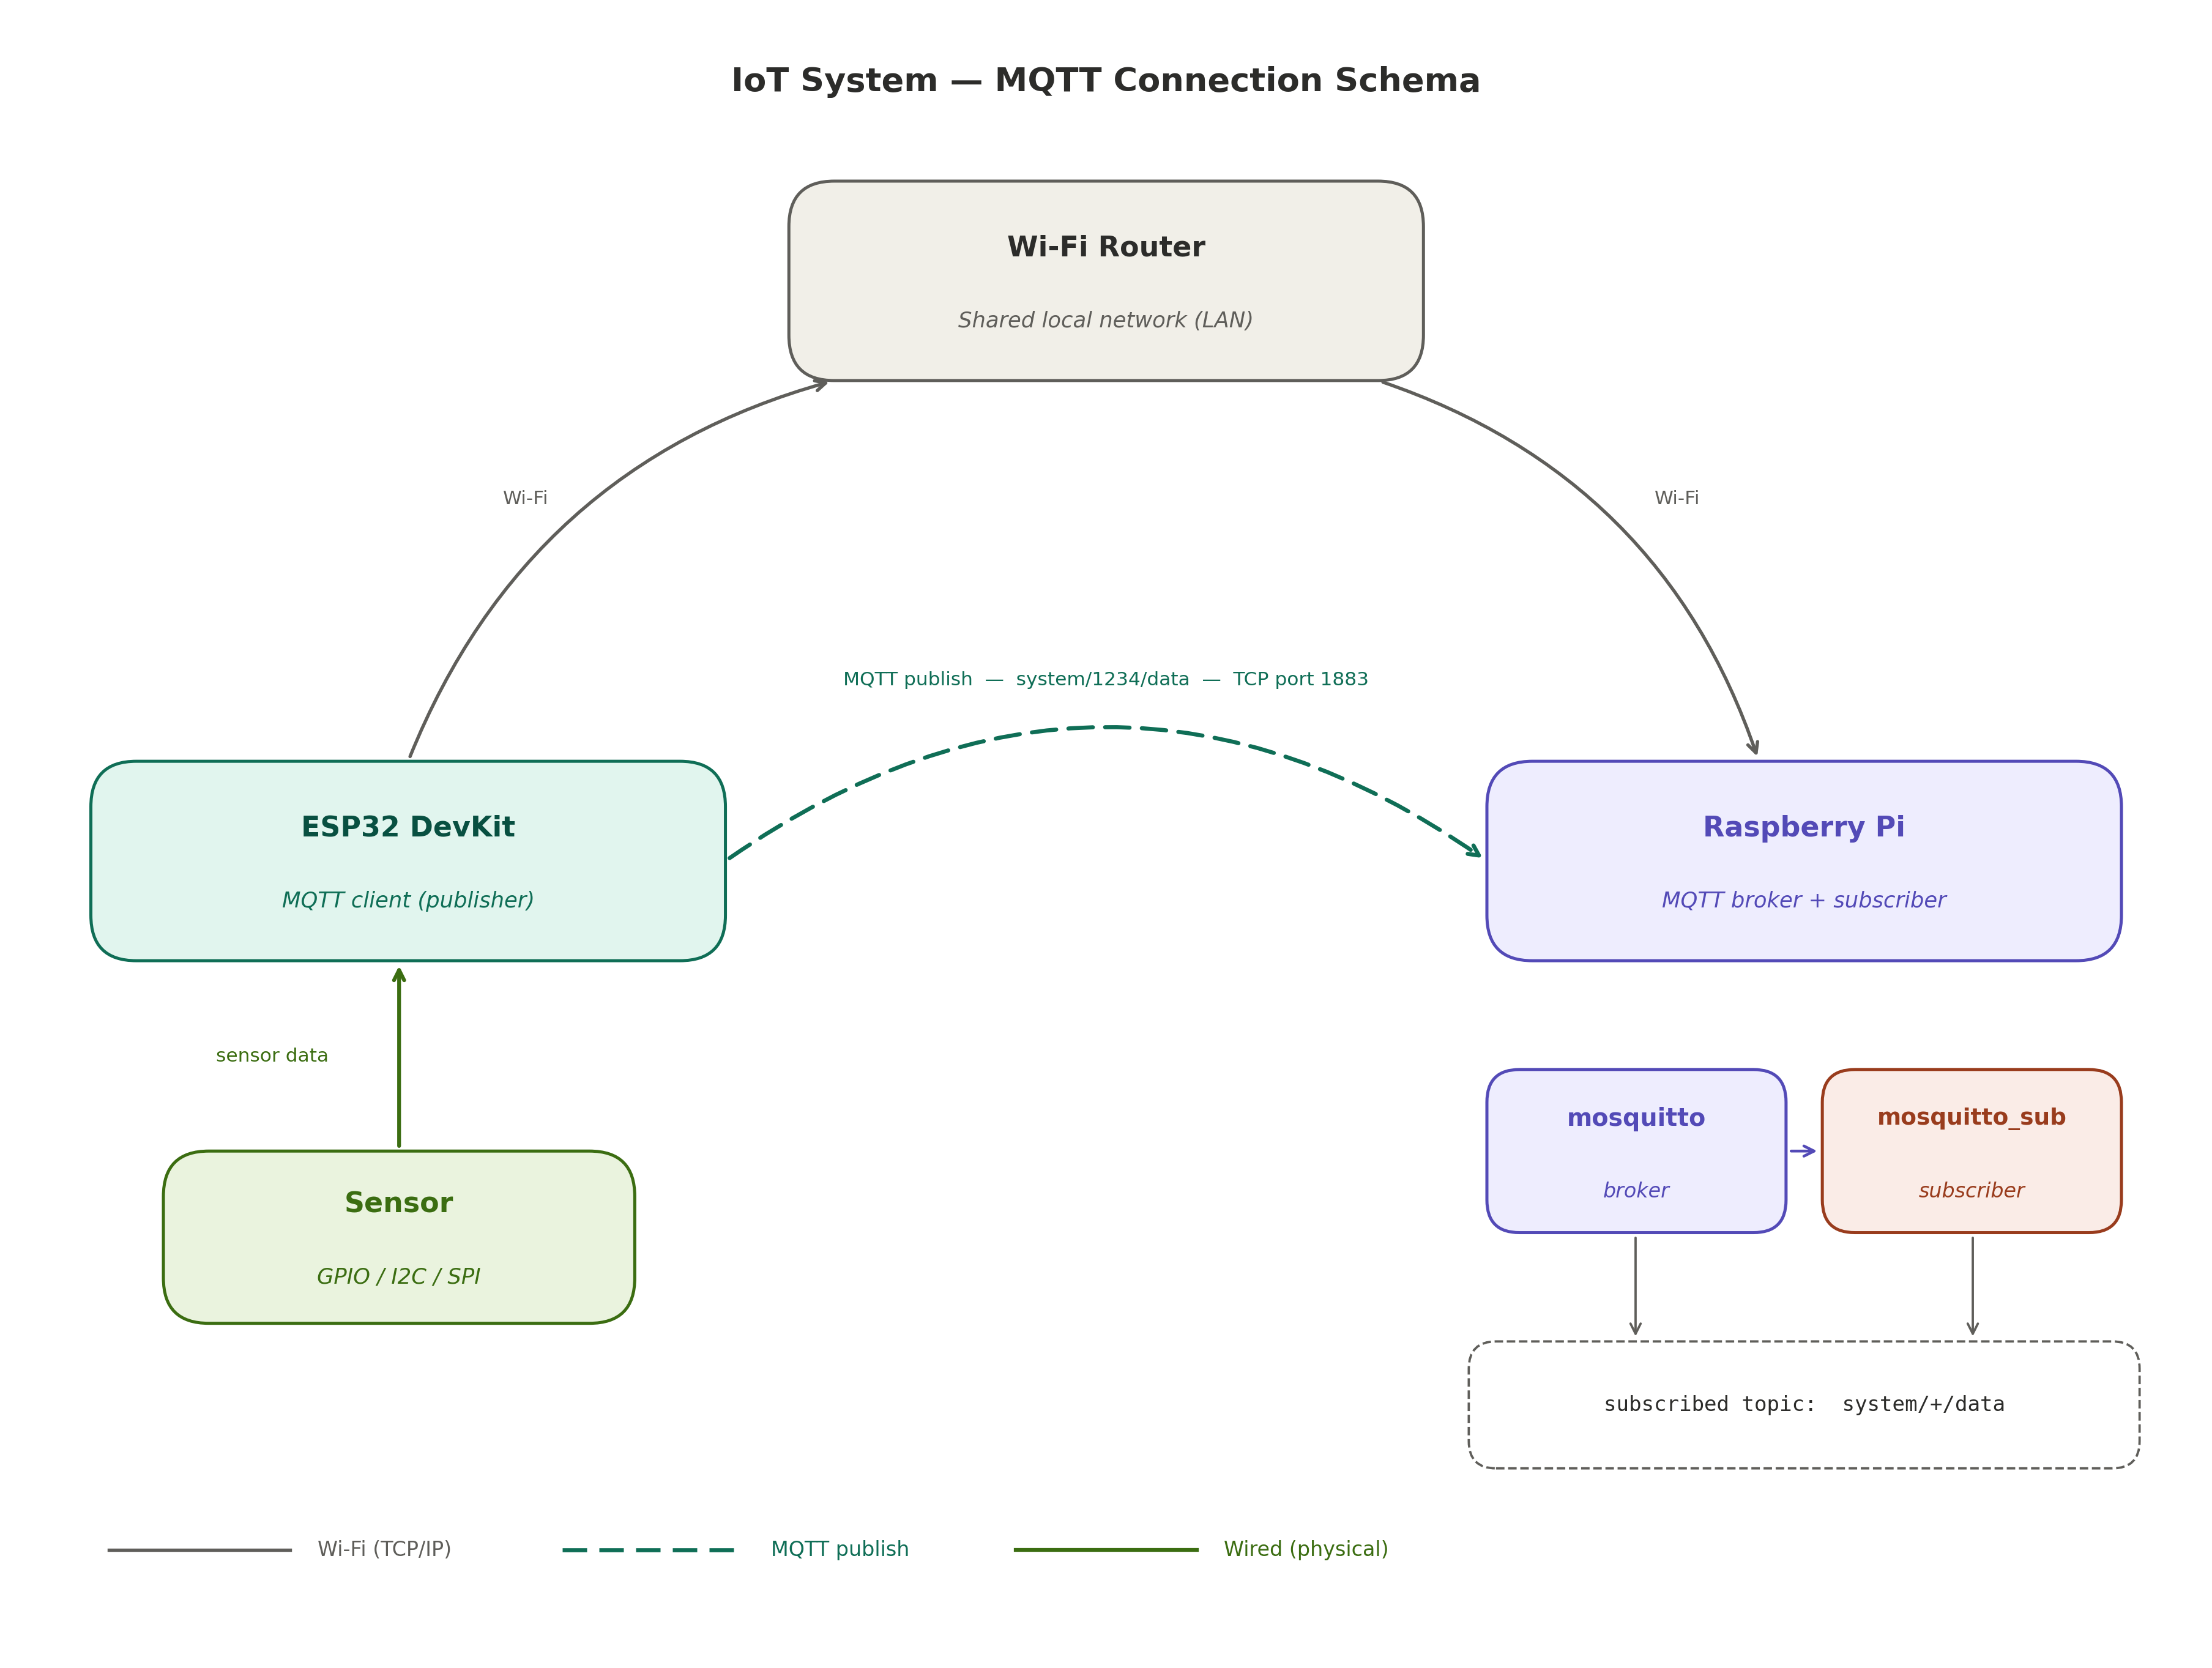
\includegraphics[width=\textwidth]{iot_mqtt_schema.png}
    \caption{IoT System — MQTT Connection Schema of the laboratory setup}
    \label{fig:iot_mqtt}
\end{figure}
% \section{Part 1 -- IoT Node with ESP32 and BME680}
% The first part focuses on building a single IoT node. An ESP32 DevKit board is connected to a BME680 environmental sensor through the SPI interface. The node is programmed to read measurements from the sensor and expose them through HTTP, so that any client on the same Wi-Fi network can request the latest values. This step is essential to understand how a microcontroller interfaces with a sensor and how it can act as a small web server.

% \section{Part 2 -- Gateway Based on Raspberry Pi with MQTT Broker}
% The second part is dedicated to the gateway. A Raspberry Pi is configured from a clean installation of Raspberry Pi OS, and the \texttt{mosquitto} MQTT broker (together with its command-line clients) is installed and tested. The gateway is meant to centralize messages produced by remote nodes, providing a publish/subscribe mechanism that is more scalable and efficient than direct HTTP requests for many real IoT scenarios.

% \section{Part 3 -- Full IoT System Integration}
% The third and final part combines the previous two. The ESP32 node publishes its sensor data through MQTT to the broker running on the Raspberry Pi, while a client on the Raspberry Pi (\texttt{mosquitto\_sub}) subscribes to the relevant topic and prints the received messages. This part demonstrates a complete IoT pipeline, from physical measurement on the node to data reception on the gateway.
The data flow can be summarized as follows:
\begin{enumerate}
    \item The BME680 sensor produces digital readings (temperature, humidity, pressure, gas resistance) and transmits them to the ESP32 over the SPI bus.
    \item The ESP32 connects to the Wi-Fi access point, packages the readings into a JSON payload and publishes them to the MQTT broker.
    \item The \texttt{mosquitto} broker on the Raspberry Pi receives the message and forwards it to all clients subscribed to the matching topic.
    \item The \texttt{mosquitto\_sub} client on the Raspberry Pi prints the received data on the console, completing the chain.
\end{enumerate}

%==================================================================
\chapter{Part 1 -- IoT Node with ESP32 and BME680}
%==================================================================
 
\section{Equipment}
The hardware and software used in the first part of the laboratory are the following:
\begin{itemize}
    \item ESP32 DevKitC (DOIT ESP32 DEVKIT V1) microcontroller board.
    \item BME680 environmental sensor (temperature, humidity, pressure and gas) -- Adafruit breakout board.
    \item Breadboard and jumper wires.
    \item USB cable (Micro-USB) for programming and powering the ESP32.
    \item Personal computer with the Arduino IDE installed.
    \item Adafruit BME680 Library for Arduino.
\end{itemize}
 
\begin{figure}[H]
    \centering
    \begin{subfigure}[b]{0.45\textwidth}
        \centering
        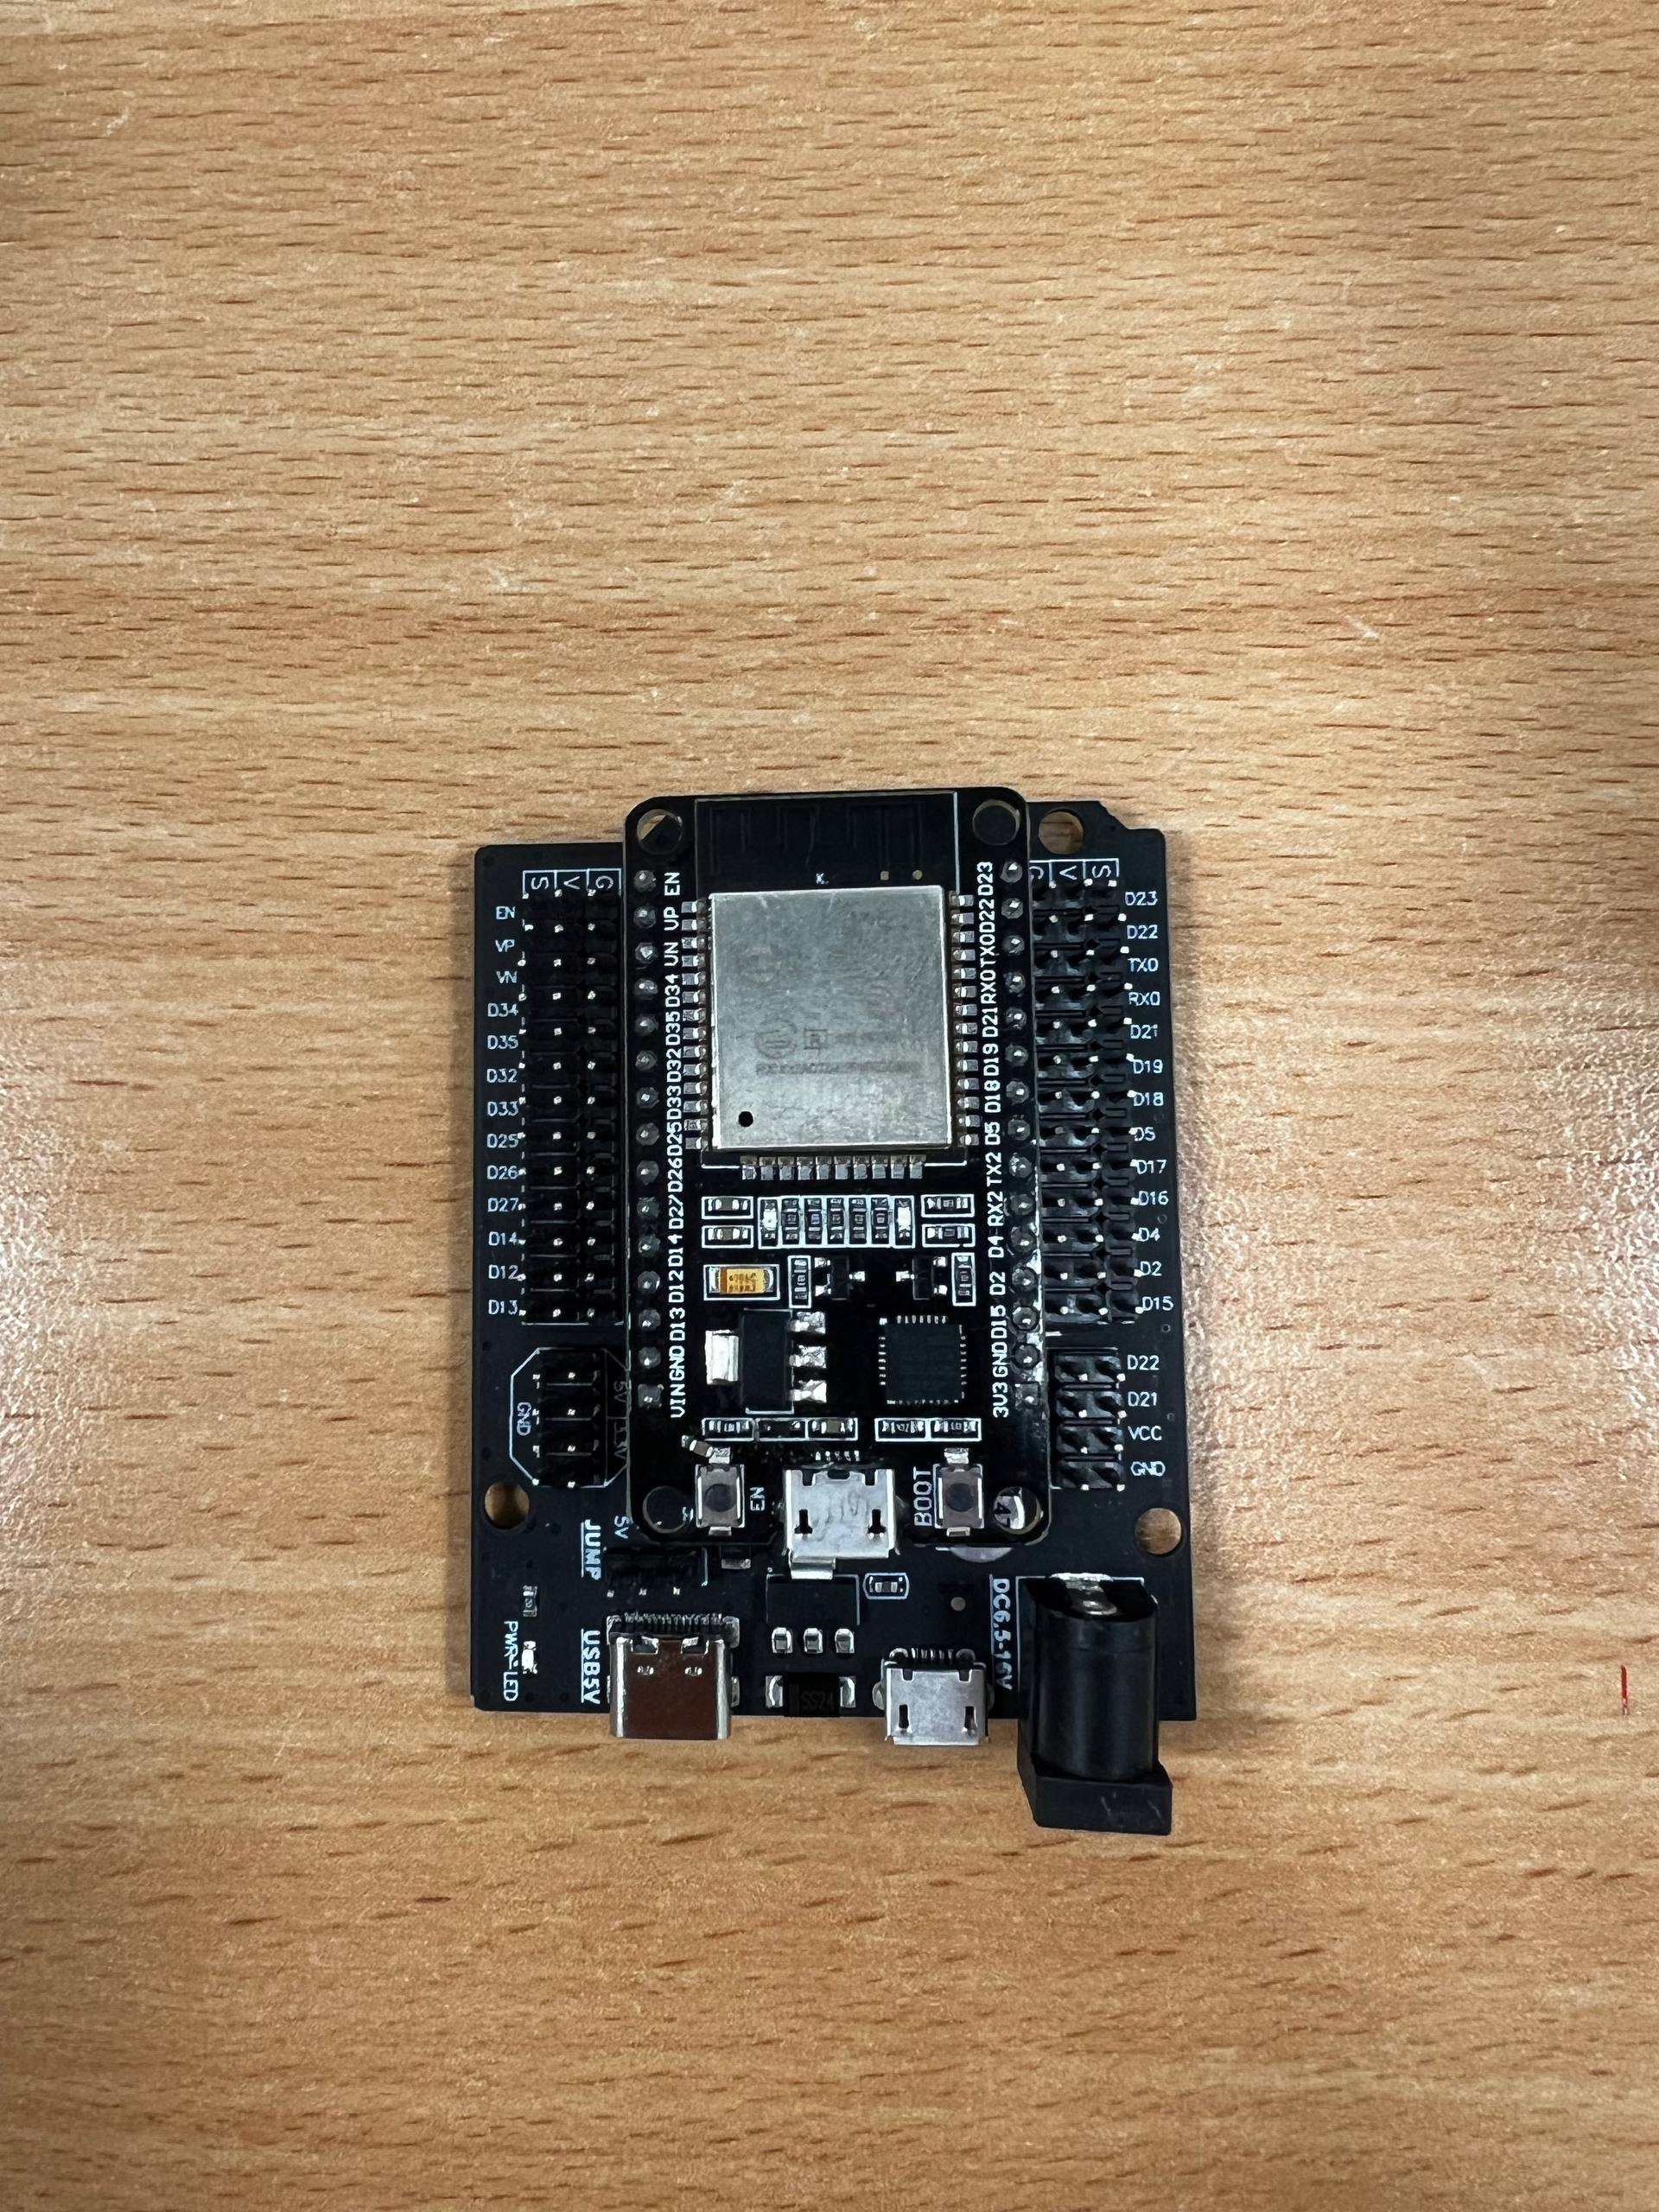
\includegraphics[width=\textwidth]{p1_esp32_board.jpg}
        \caption{ESP32 DevKitC (DOIT V1).}
        \label{fig:p1_esp32_board}
    \end{subfigure}
    \hfill
    \begin{subfigure}[b]{0.45\textwidth}
        \centering
        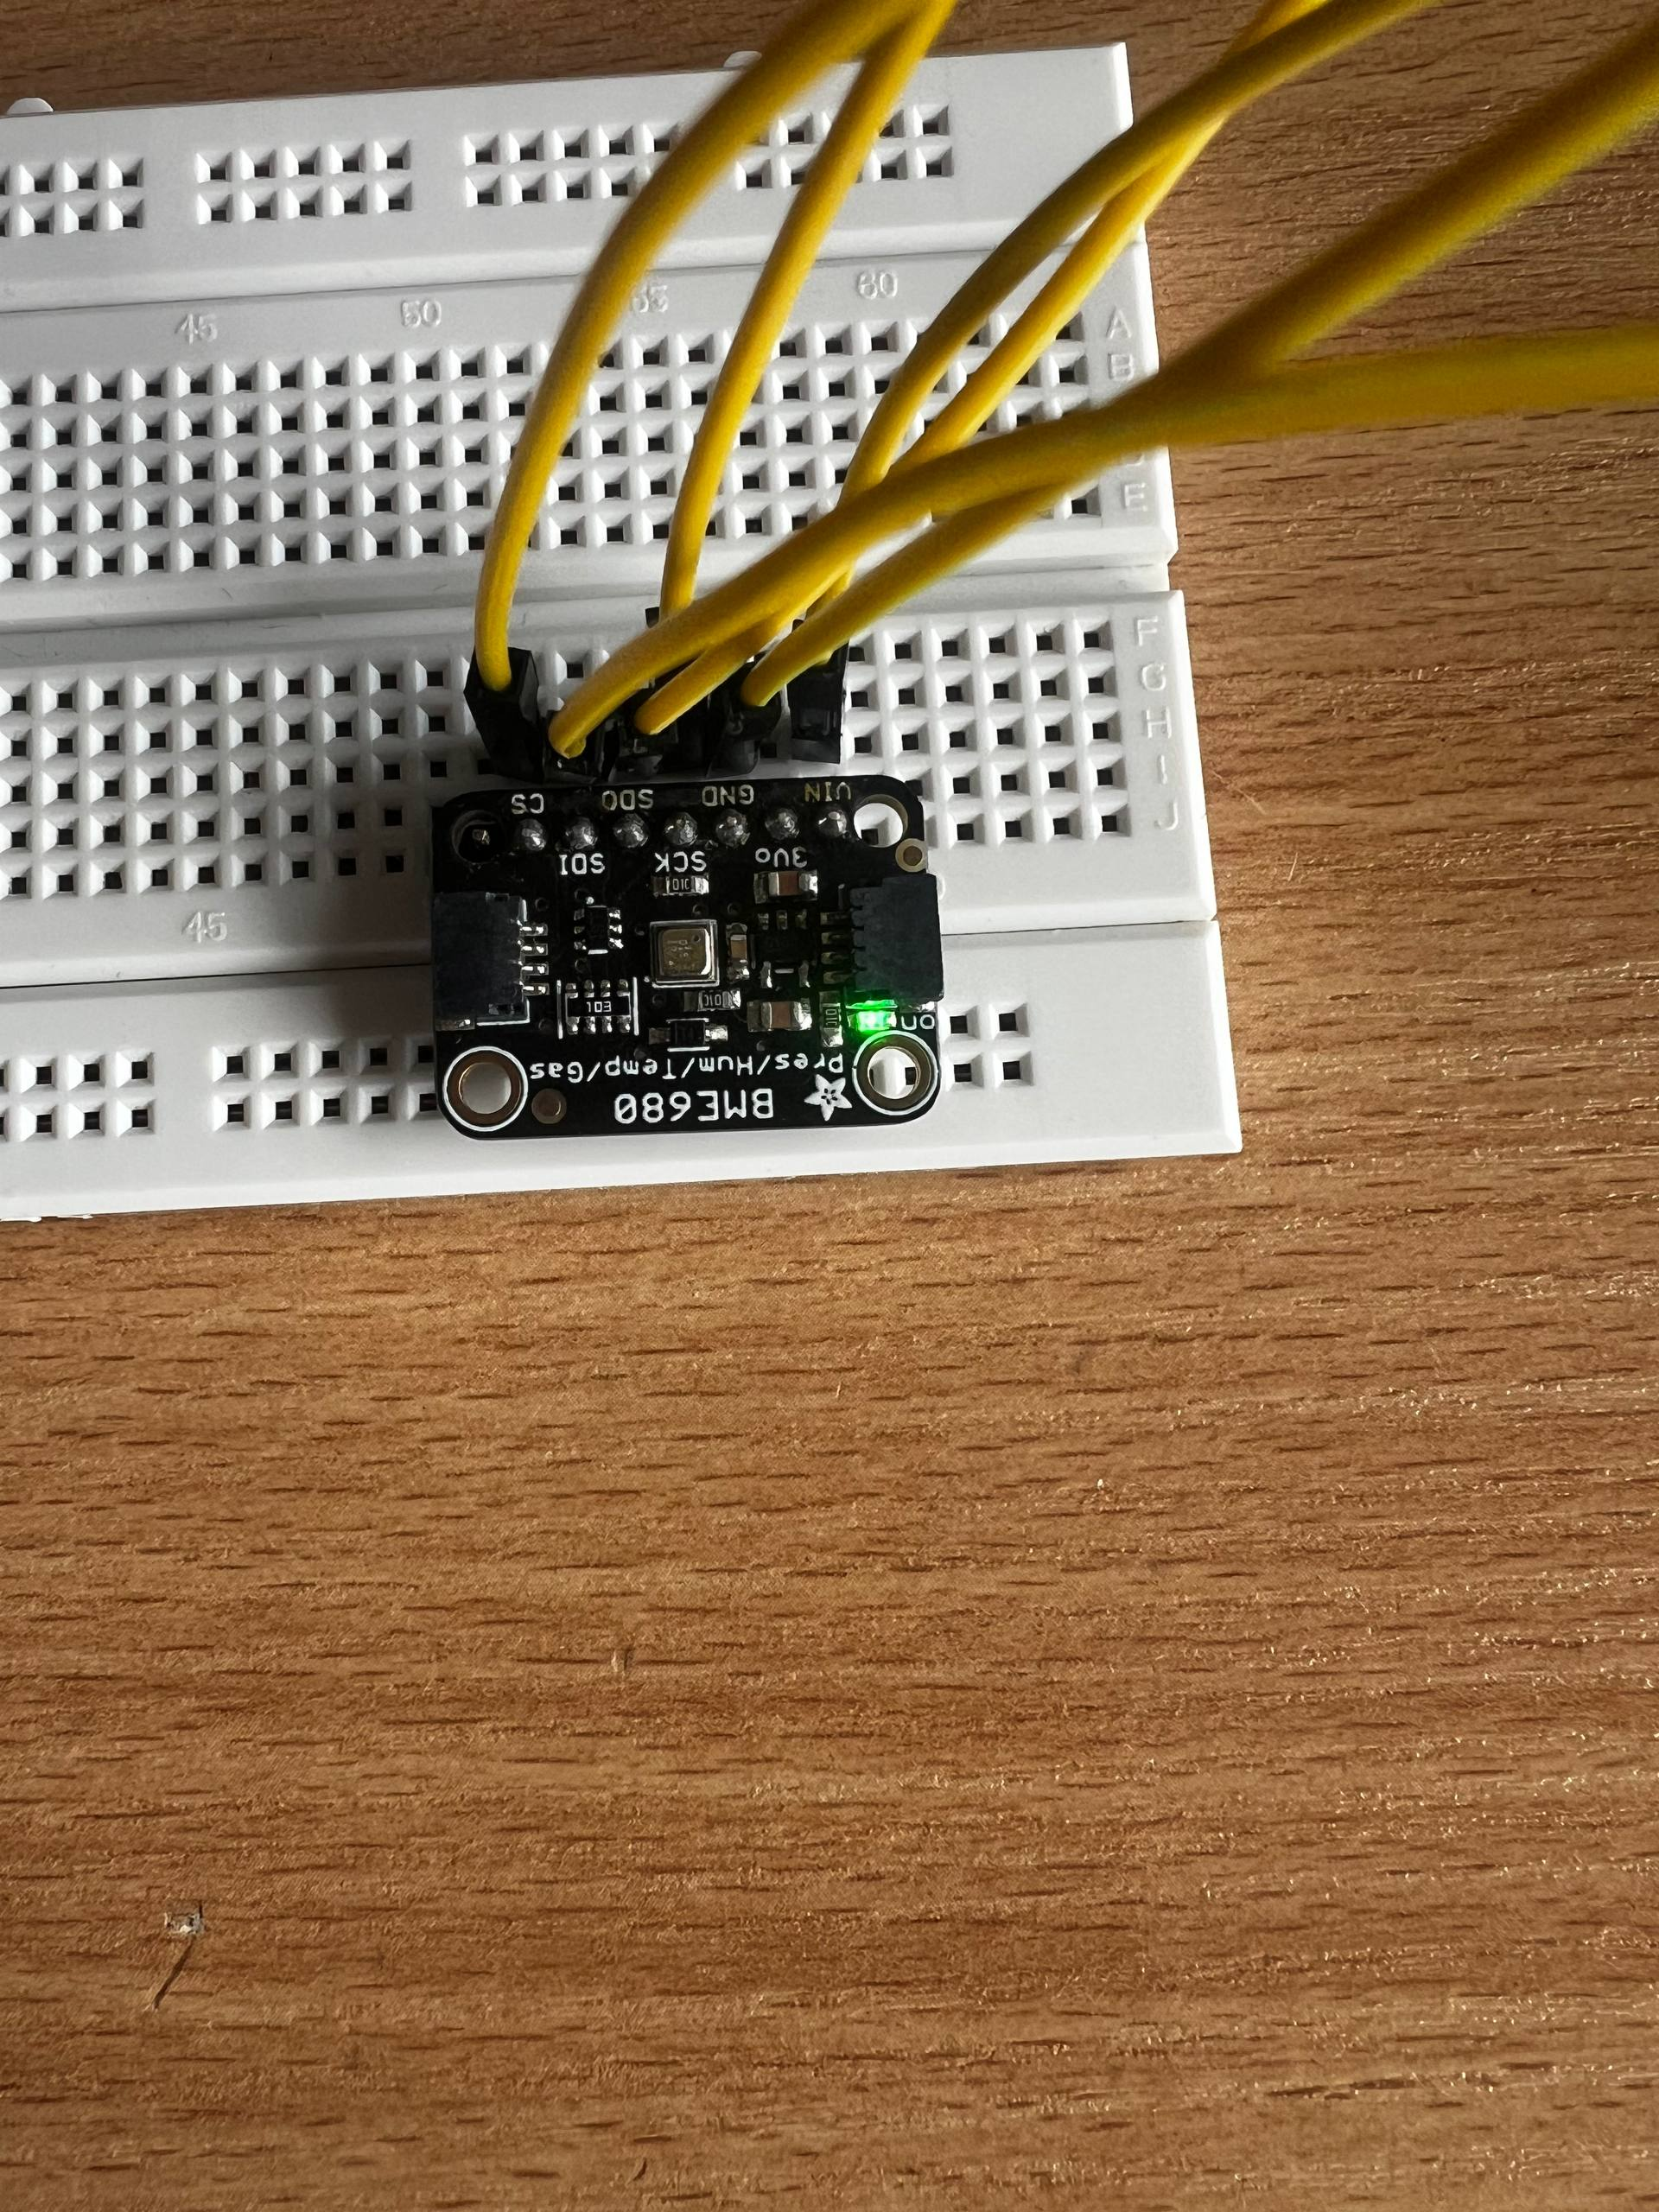
\includegraphics[width=\textwidth]{p1_bme680_sensor.jpg}
        \caption{Adafruit BME680 sensor on breadboard.}
        \label{fig:p1_bme680_sensor}
    \end{subfigure}
    \caption{Main hardware components used in Part 1.}
    \label{fig:p1_components}
\end{figure}
 
The connections between the ESP32 and the BME680 sensor follow the SPI scheme summarized in Table~\ref{tab:esp32_bme680}.
 
\begin{table}[H]
    \centering
    \caption{Connection list between ESP32 and BME680.}
    \label{tab:esp32_bme680}
    \begin{tabular}{ll}
        \toprule
        \textbf{ESP32 pin} & \textbf{BME680 pin} \\
        \midrule
        Vin                 & Vin \\
        do not connect!     & 3Vo (leave unconnected) \\
        GND                 & GND \\
        D18                 & SCK \\
        D19                 & SDO \\
        D23                 & SDI \\
        D5                  & CS \\
        \bottomrule
    \end{tabular}
\end{table}
 
\section{Hardware Connections}
 
\begin{figure}[H]
    \centering
    \begin{subfigure}[b]{0.48\textwidth}
        \centering
        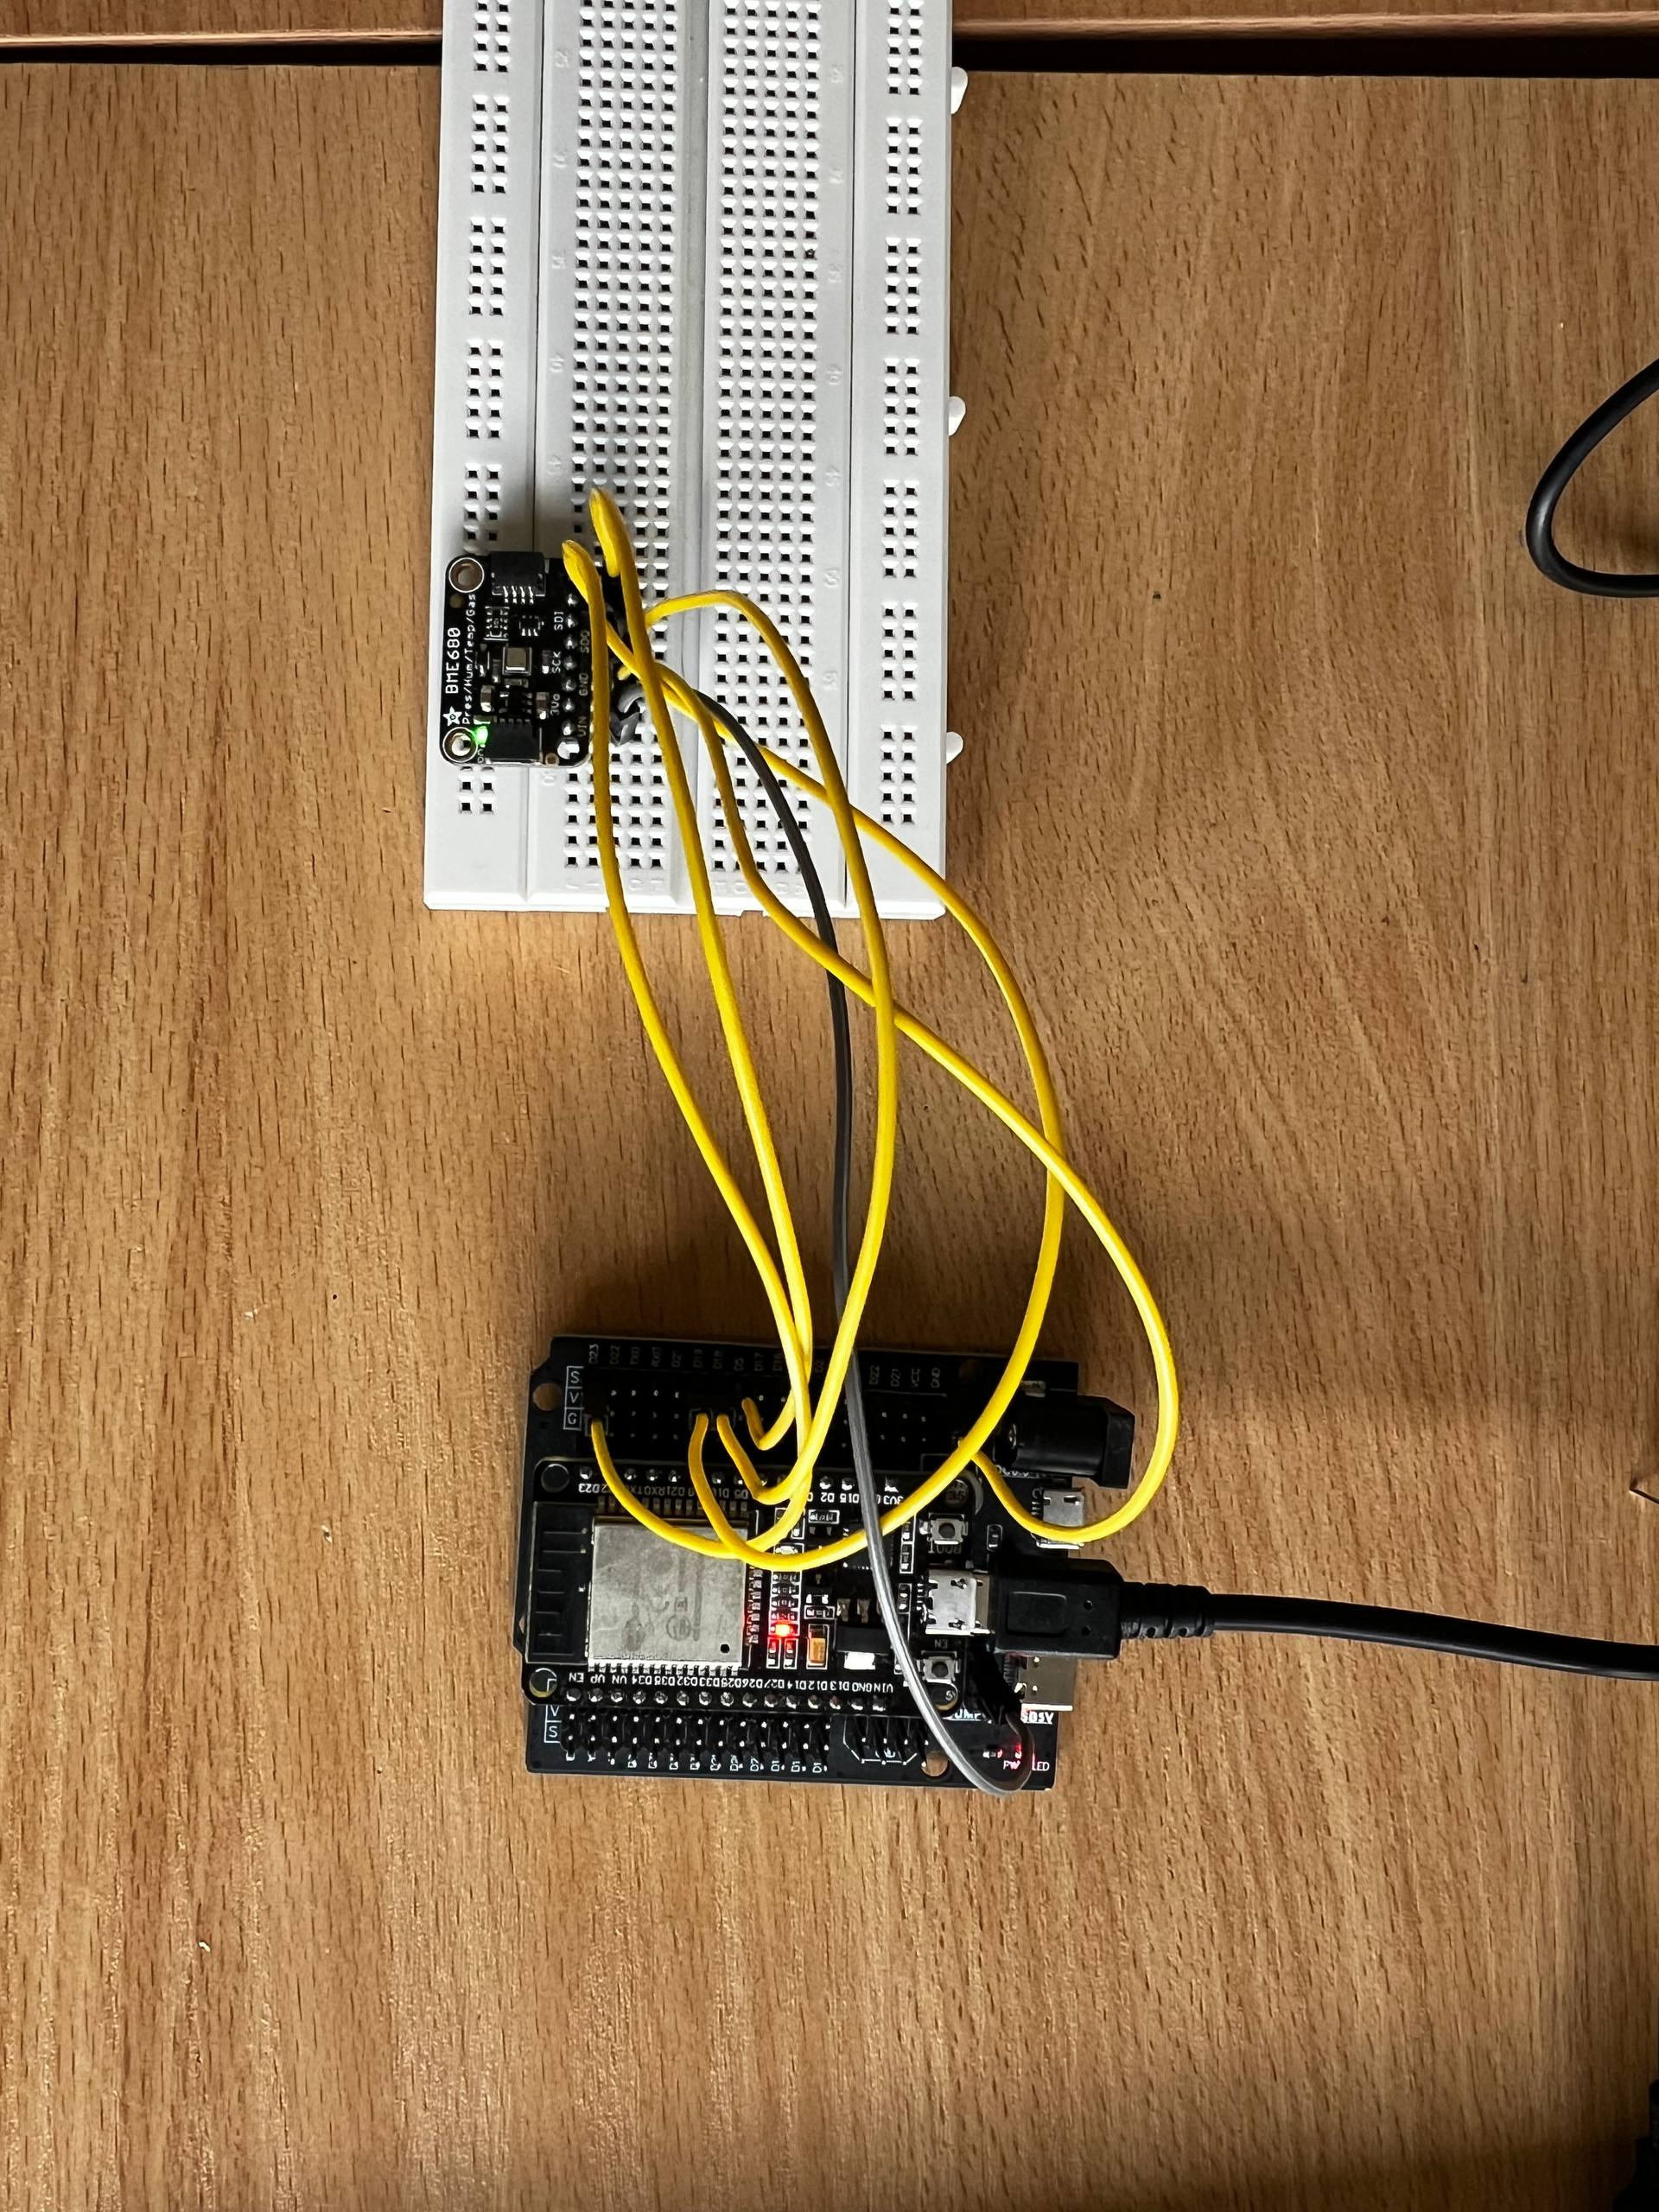
\includegraphics[width=\textwidth]{p1_wiring_alt.jpg}
        \caption{Top view of the wiring.}
        \label{fig:p1_wiring_full}
    \end{subfigure}
    \hfill
    \begin{subfigure}[b]{0.48\textwidth}
        \centering
        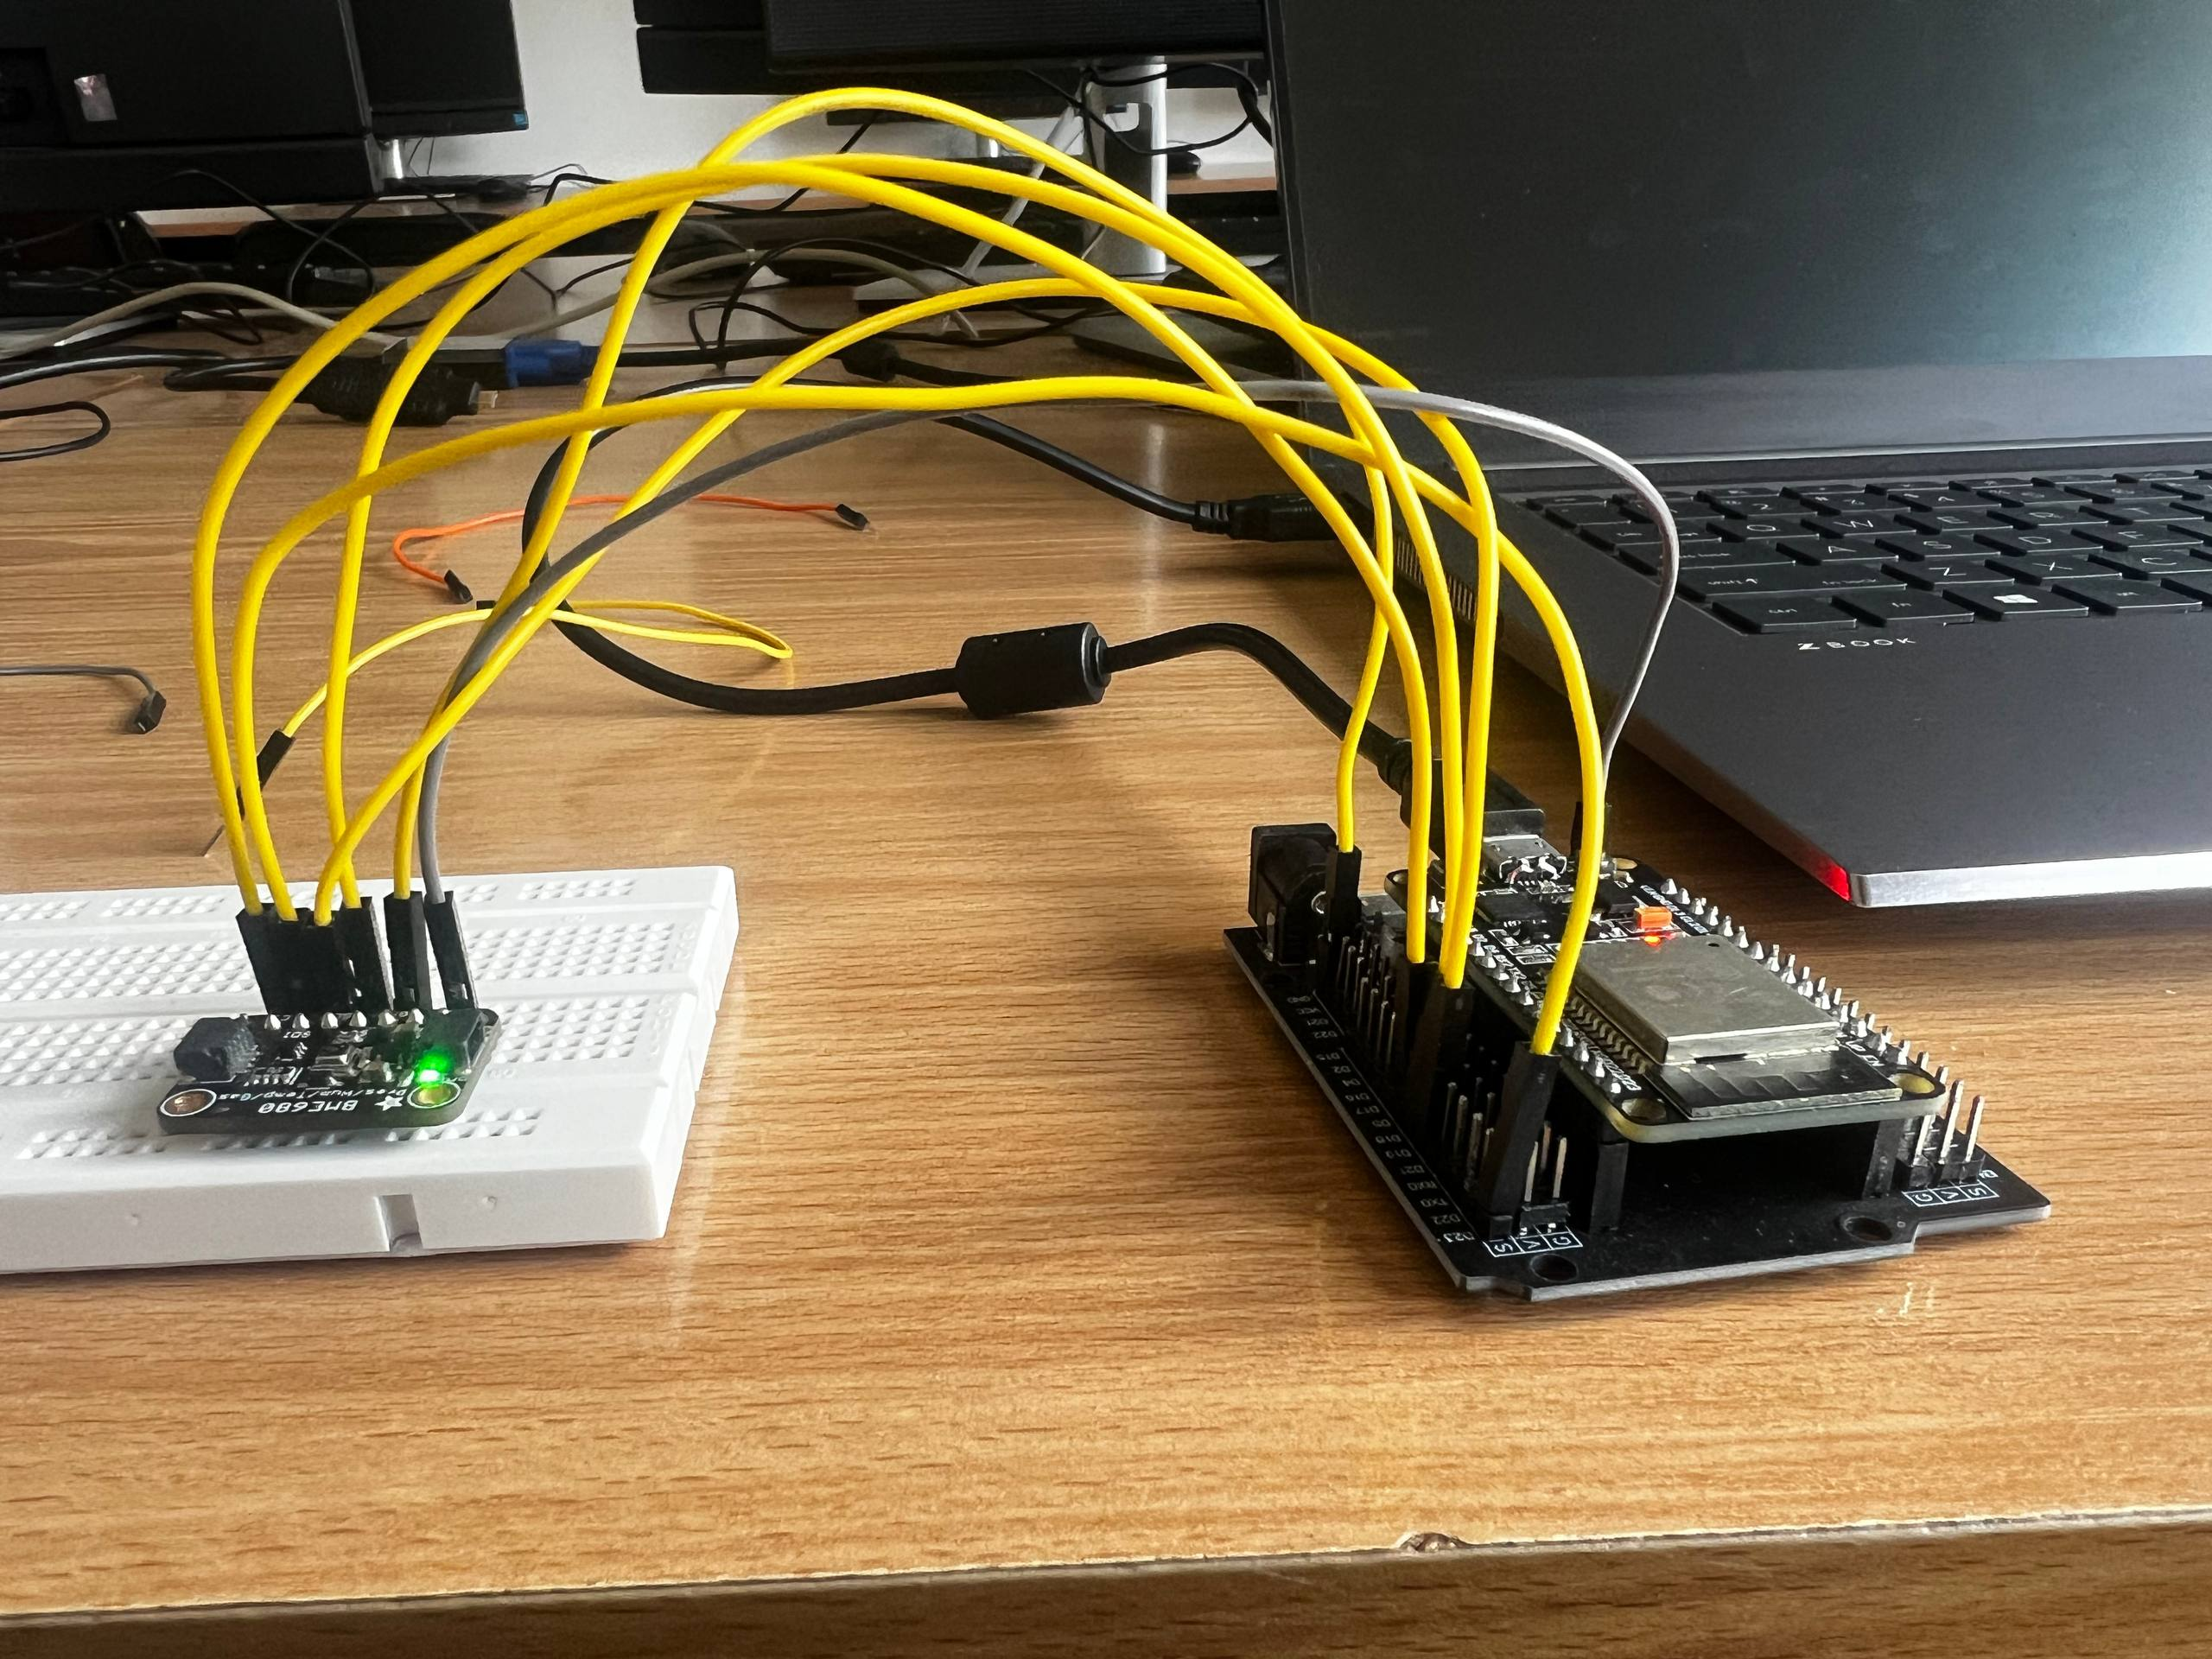
\includegraphics[width=\textwidth]{p1_alt_angle_wiring.jpg}
        \caption{Alternative angle of the wiring.}
        \label{fig:p1_wiring_alt}
    \end{subfigure}
    \caption{Hardware connection between the ESP32 DevKit and the BME680 sensor on the breadboard. The yellow wires implement the SPI bus (SCK, SDO, SDI, CS), while the black/white wires carry power (Vin) and ground (GND).}
    \label{fig:p1_wiring}
\end{figure}
 
\section{Code Description}
 
The firmware for Part 1 was developed in three incremental sub-steps. Each sub-step extends the previous one, allowing each block (sensor, Wi-Fi server, and their integration) to be tested independently before being merged into the final node firmware.
 
\subsection{Sub-step 1: BME680 Sensor Reading}
The first sub-step is built on top of the example \texttt{bme680test} provided by the Adafruit BME680 Library. The example was modified by:
\begin{itemize}
    \item changing the definition of \texttt{BME\_CS} to \texttt{5},
    \item commenting the line that uses the I2C constructor (\texttt{Adafruit\_BME680 bme(\&Wire);}),
    \item uncommenting the line that uses the SPI constructor with chip-select pin (\texttt{Adafruit\_BME680 bme(BME\_CS);}).
\end{itemize}
The code initializes the sensor over hardware SPI, configures oversampling and filtering options, and prints the four physical measurements (temperature, pressure, humidity, gas resistance) plus the estimated altitude on the Serial Monitor every two seconds.
 
\begin{lstlisting}[language=C++, caption={Sub-step 1 -- BME680 sensor reading over SPI.}]
#include <Wire.h>
#include <SPI.h>
#include <Adafruit_Sensor.h>
#include "Adafruit_BME680.h"
 
#define BME_SCK 13
#define BME_MISO 12
#define BME_MOSI 11
#define BME_CS 5
 
#define SEALEVELPRESSURE_HPA (1013.25)
 
//Adafruit_BME680 bme(&Wire); // I2C
//Adafruit_BME680 bme(&Wire1); // example of I2C on another bus
Adafruit_BME680 bme(BME_CS); // hardware SPI
//Adafruit_BME680 bme(BME_CS, BME_MOSI, BME_MISO,  BME_SCK);
 
void setup() {
  Serial.begin(9600);
  while (!Serial);
  Serial.println(F("BME680 test"));
 
  if (!bme.begin()) {
    Serial.println("Could not find a valid BME680 sensor, check wiring!");
    while (1);
  }
 
  // Set up oversampling and filter initialization
  bme.setTemperatureOversampling(BME680_OS_8X);
  bme.setHumidityOversampling(BME680_OS_2X);
  bme.setPressureOversampling(BME680_OS_4X);
  bme.setIIRFilterSize(BME680_FILTER_SIZE_3);
  bme.setGasHeater(320, 150); // 320*C for 150 ms
}
 
void loop() {
  if (! bme.performReading()) {
    Serial.println("Failed to perform reading :(");
    return;
  }
  Serial.print("Temperature = ");
  Serial.print(bme.temperature);
  Serial.println(" *C");
 
  Serial.print("Pressure = ");
  Serial.print(bme.pressure / 100.0);
  Serial.println(" hPa");
 
  Serial.print("Humidity = ");
  Serial.print(bme.humidity);
  Serial.println(" %");
 
  Serial.print("Gas = ");
  Serial.print(bme.gas_resistance / 1000.0);
  Serial.println(" KOhms");
 
  Serial.print("Approx. Altitude = ");
  Serial.print(bme.readAltitude(SEALEVELPRESSURE_HPA));
  Serial.println(" m");
 
  Serial.println();
  delay(2000);
}
\end{lstlisting}
 
The Arduino IDE Serial Monitor confirmed that the BME680 sensor was correctly initialized and that all four measurements were available with stable values, as shown in Figure~\ref{fig:p1_serial_bme680}.
 
\begin{figure}[H]
    \centering
    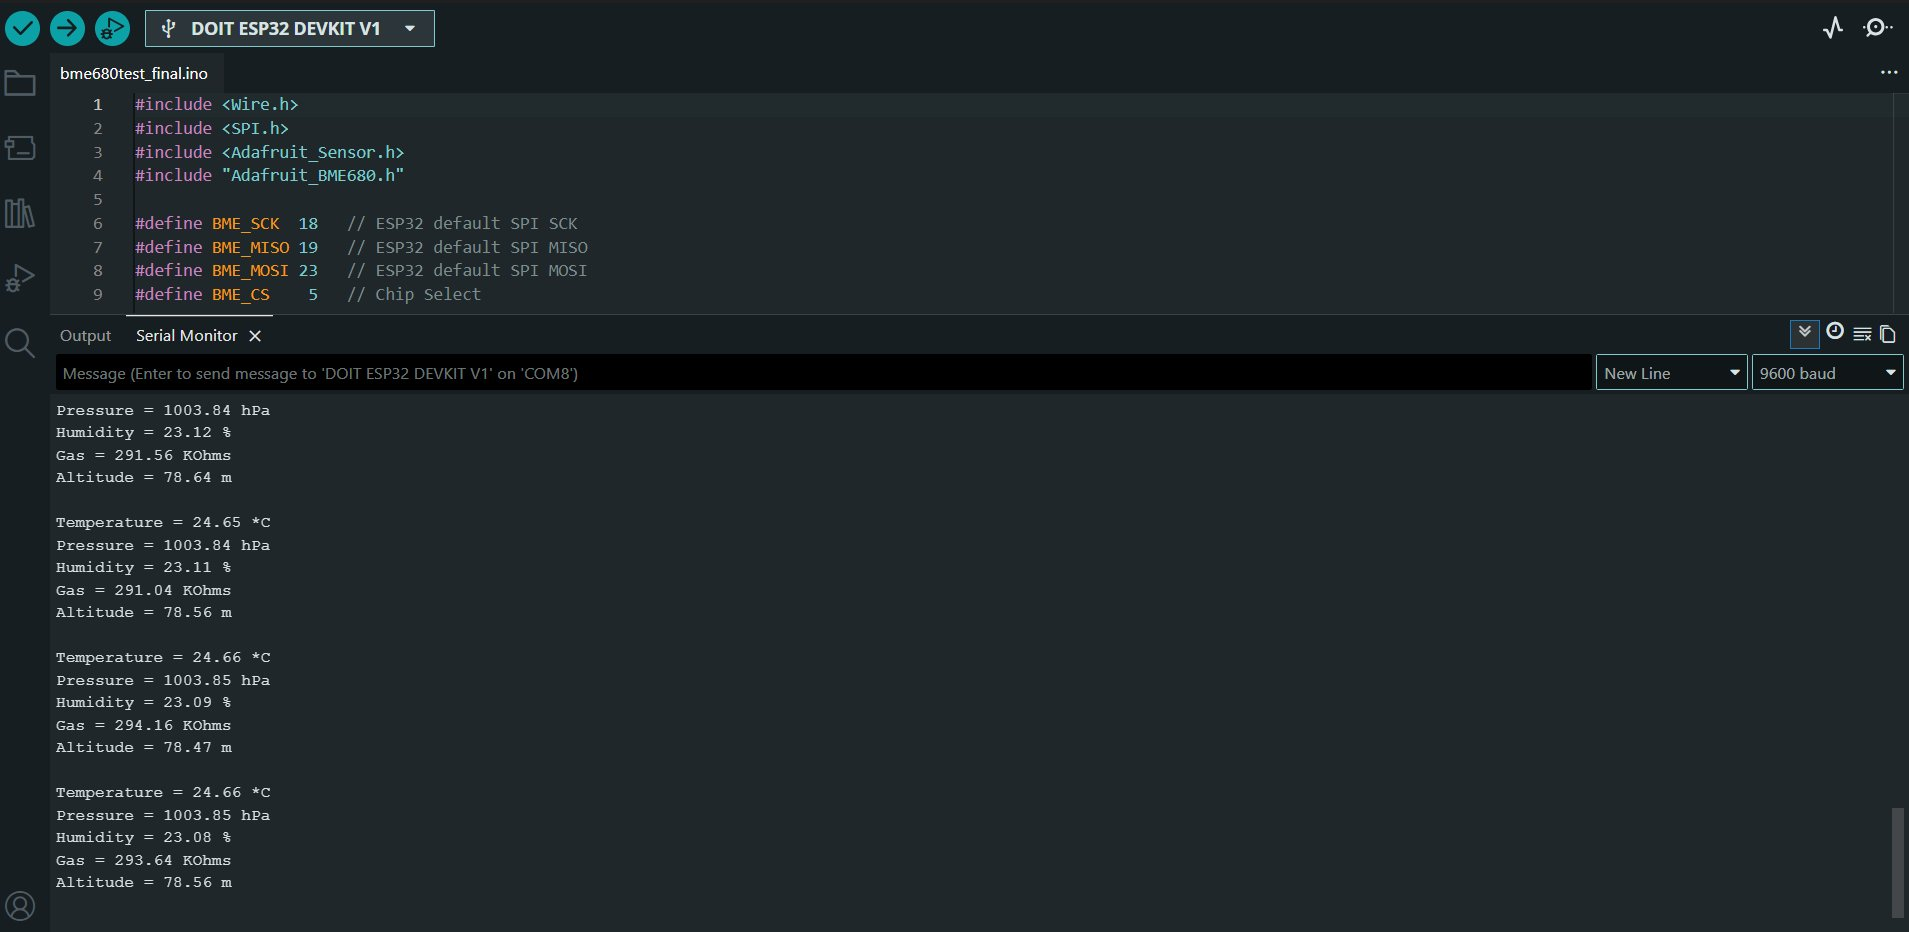
\includegraphics[width=0.95\textwidth]{p1_serial_bme680.png}
    \caption{Sub-step 1: Serial Monitor output showing the BME680 readings (temperature, pressure, humidity, gas resistance and altitude).}
    \label{fig:p1_serial_bme680}
\end{figure}
 
\subsection{Sub-step 2: Wi-Fi Access Point and HTTP Server}
The second sub-step is based on the \texttt{SimpleWiFiServer} example from the ESP32 Wi-Fi library. Instead of connecting to an external access point, the ESP32 is configured to create its own Wi-Fi access point (\texttt{ESP32-AP}, password \texttt{12345678}) and start a web server on port 80. The page returned by the server contains two hyperlinks (\texttt{/H} and \texttt{/L}) that allow the user to turn on or off an LED connected to pin~5 of the ESP32. This sub-step validates both the Wi-Fi soft-AP functionality and the HTTP request parsing.
 
\begin{lstlisting}[language=C++, caption={Sub-step 2 -- Wi-Fi access point and simple HTTP server.}]
#include <Arduino.h>
#include <WiFi.h>
 
const char *ssid     = "ESP32-AP";       
const char *password = "12345678";       // Min 8 characters
 
NetworkServer server(80);
 
void setup() {
  Serial.begin(115200);
  pinMode(5, OUTPUT);
 
  delay(10);
  Serial.println();
 
  // Start Access Point
  Serial.print("Starting Access Point: ");
  Serial.println(ssid);
 
  WiFi.softAP(ssid, password);
 
  IPAddress IP = WiFi.softAPIP();
  Serial.println("AP started!");
  Serial.print("IP address: ");
  Serial.println(IP);
 
  server.begin();
  Serial.println("Server started!");
}
 
void loop() {
  NetworkClient client = server.accept();
 
  if (client) {
    Serial.println("New Client.");
    String currentLine = "";
 
    while (client.connected()) {
      if (client.available()) {
        char c = client.read();
        Serial.write(c);
 
        if (c == '\n') {
          if (currentLine.length() == 0) {
            client.println("HTTP/1.1 200 OK");
            client.println("Content-type:text/html");
            client.println();
 
            client.print("Click <a href=\"/H\">here</a> to turn LED on pin 5 ON.<br>");
            client.print("Click <a href=\"/L\">here</a> to turn LED on pin 5 OFF.<br>");
 
            client.println();
            break;
          } else {
            currentLine = "";
          }
        } else if (c != '\r') {
          currentLine += c;
        }
 
        if (currentLine.endsWith("GET /H")) {
          digitalWrite(5, HIGH);
        }
        if (currentLine.endsWith("GET /L")) {
          digitalWrite(5, LOW);
        }
      }
    }
 
    client.stop();
    Serial.println("Client Disconnected.");
  }
}
\end{lstlisting}
 
The serial output of this sub-step (Figure~\ref{fig:p1_serial_http}) shows the ESP32 correctly accepting HTTP connections from a client, parsing the standard HTTP request headers, and serving the simple HTML page on the address \texttt{192.168.4.1} (Figure~\ref{fig:p1_browser_simple}).
 
\begin{figure}[H]
    \centering
    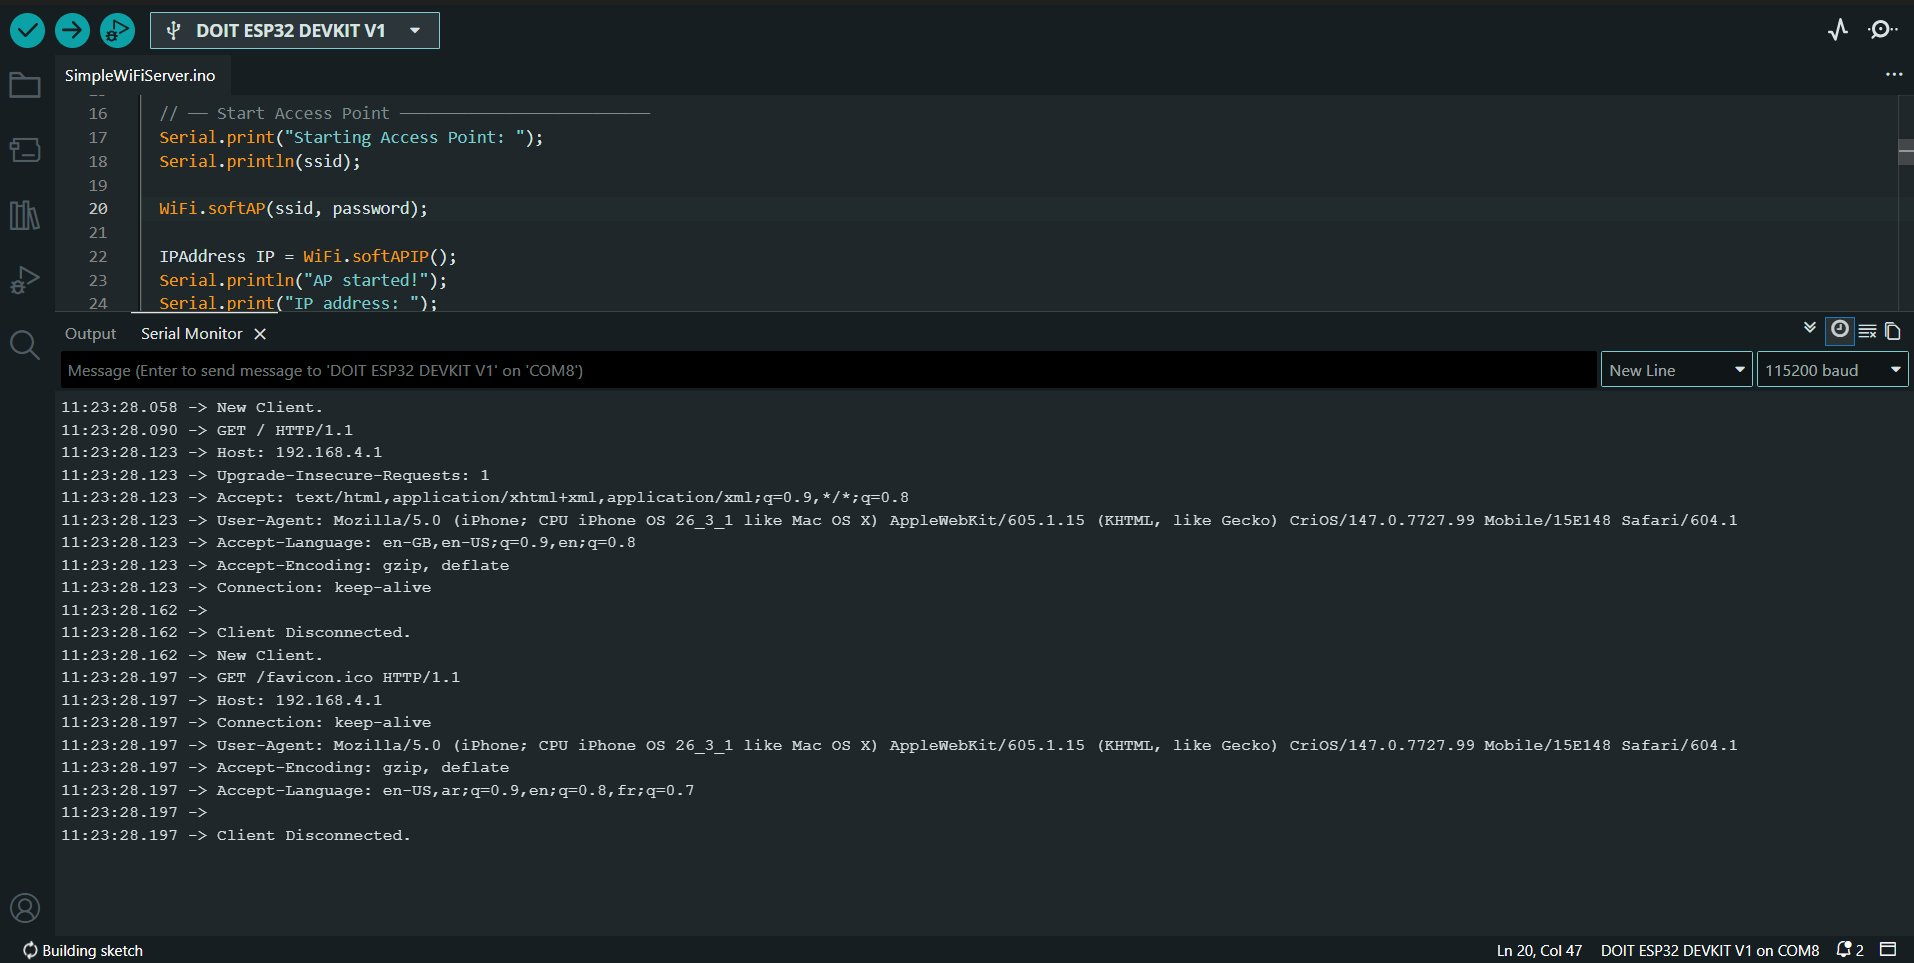
\includegraphics[width=0.95\textwidth]{p1_serial_http.png}
    \caption{Sub-step 2: Serial Monitor showing the parsed HTTP request headers received by the ESP32.}
    \label{fig:p1_serial_http}
\end{figure}
 
\begin{figure}[H]
    \centering
    \fbox{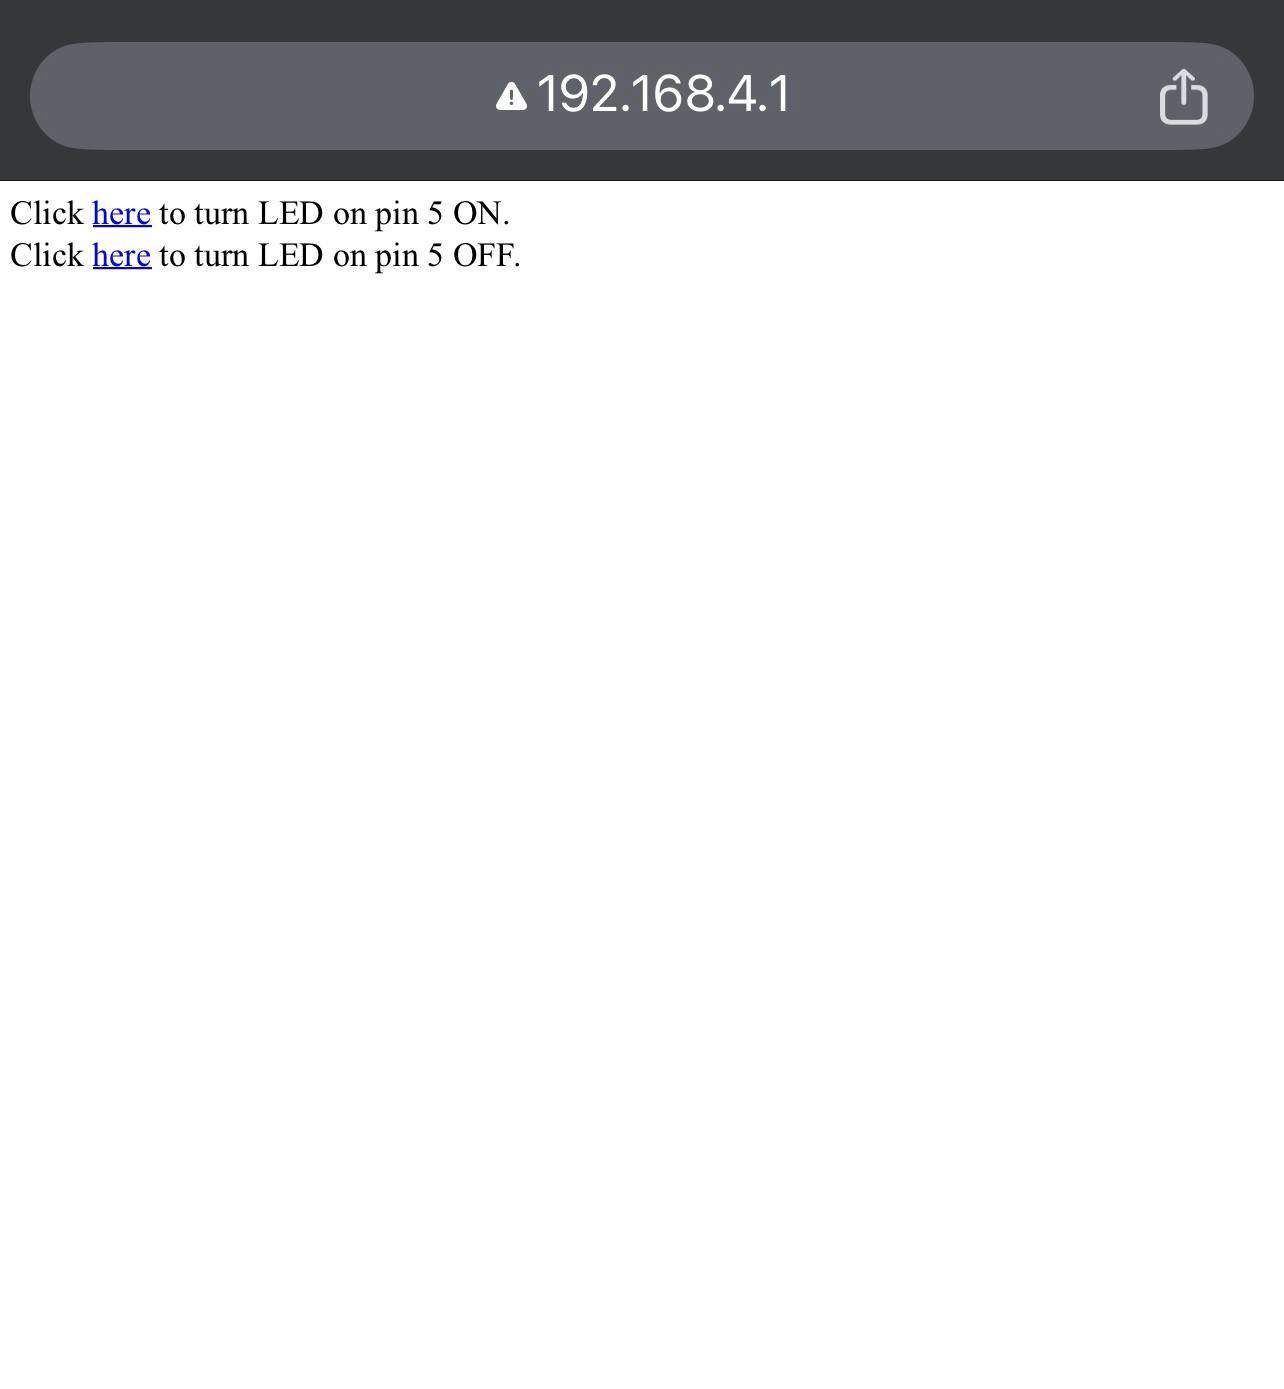
\includegraphics[width=0.6\textwidth]{images/p1_browser_simple.jpg}}
    \caption{Sub-step 2: simple HTML page served by the ESP32 on \texttt{192.168.4.1}.}
    \label{fig:p1_browser_simple}
\end{figure}
 
\subsection{Sub-step 3: Combined Sensor Node with Web Dashboard}
In the final sub-step, the BME680 reading code from Sub-step~1 was merged with the Wi-Fi web server from Sub-step~2. The resulting firmware exposes a complete web dashboard on port~80: each HTTP request returns an HTML page containing the latest temperature, humidity, pressure, gas resistance and altitude readings, together with two buttons to control an LED. The page automatically refreshes every five seconds, providing a near real-time view of the environmental conditions. CSS styling is embedded directly in the HTML for a clean and responsive layout.
 
\begin{lstlisting}[language=C++, caption={Sub-step 3 -- Combined BME680 sensor + Wi-Fi dashboard with LED control.}]
#include <Arduino.h>
#include <Wire.h>
#include <SPI.h>
#include <Adafruit_Sensor.h>
#include "Adafruit_BME680.h"
#include <WiFi.h>
 
// WiFi AP Credentials
const char *ssid     = "ESP32-BME680";
const char *password = "12345678";
 
// BME680 SPI Setup
#define BME_CS 5
#define SEALEVELPRESSURE_HPA (1013.25)
Adafruit_BME680 bme(BME_CS);
 
// LED Pin
#define LED_PIN 2   // Built-in LED on most ESP32 boards
 
// Web Server
NetworkServer server(80);
 
// Build HTML Page
String buildPage(bool ledState) {
  if (!bme.performReading()) {
    return "<h2>Failed to read BME680!</h2>";
  }
 
  String html = "<!DOCTYPE html><html><head>";
  html += "<meta charset='UTF-8'>";
  html += "<meta http-equiv='refresh' content='5'>";
  html += "<title>ESP32 BME680</title>";
  html += "<style>";
  html += "  body { font-family: Arial; text-align: center; background: #f0f0f0; margin: 0; padding: 20px; }";
  html += "  h1 { color: #333; }";
  html += "  .card { background: white; border-radius: 12px; padding: 20px;";
  html += "          margin: 15px auto; max-width: 300px; box-shadow: 0 2px 8px rgba(0,0,0,0.1); }";
  html += "  .value { font-size: 2em; font-weight: bold; color: #e67e22; }";
  html += "  .label { color: #888; font-size: 0.9em; margin-bottom: 5px; }";
  html += "  .btn { display: inline-block; padding: 12px 30px; margin: 8px;";
  html += "         border-radius: 8px; text-decoration: none; font-size: 1em; font-weight: bold; }";
  html += "  .btn-on  { background: #2ecc71; color: white; }";
  html += "  .btn-off { background: #e74c3c; color: white; }";
  html += "  .led-status { font-size: 1.1em; margin-top: 10px; }";
  html += "</style></head><body>";
 
  html += "<h1>ESP32 BME680 Monitor</h1>";
 
  // Sensor Cards
  html += "<div class='card'><div class='label'>Temperature</div>";
  html += "<div class='value'>" + String(bme.temperature, 1) + " C</div></div>";
 
  html += "<div class='card'><div class='label'>Humidity</div>";
  html += "<div class='value'>" + String(bme.humidity, 1) + " %</div></div>";
 
  html += "<div class='card'><div class='label'>Pressure</div>";
  html += "<div class='value'>" + String(bme.pressure / 100.0, 1) + " hPa</div></div>";
 
  html += "<div class='card'><div class='label'>Gas Resistance</div>";
  html += "<div class='value'>" + String(bme.gas_resistance / 1000.0, 1) + " KOhm</div></div>";
 
  html += "<div class='card'><div class='label'>Altitude</div>";
  html += "<div class='value'>" + String(bme.readAltitude(SEALEVELPRESSURE_HPA), 1) + " m</div></div>";
 
  // LED Control Card
  html += "<div class='card'>";
  html += "<div class='label'>LED Control</div>";
  html += "<div class='led-status'>Status: <strong>" + String(ledState ? "ON" : "OFF") + "</strong></div>";
  html += "<br>";
  html += "<a href='/H' class='btn btn-on'>Turn ON</a>";
  html += "<a href='/L' class='btn btn-off'>Turn OFF</a>";
  html += "</div>";
 
  html += "<p style='color:#aaa; font-size:0.85em;'>Auto-refreshes every 5 seconds</p>";
  html += "</body></html>";
 
  return html;
}
 
void setup() {
  Serial.begin(9600);
  delay(2000);
 
  pinMode(LED_PIN, OUTPUT);
  digitalWrite(LED_PIN, LOW);
 
  // BME680 Init
  if (!bme.begin()) {
    Serial.println("BME680 not found! Check wiring.");
    while (1);
  }
  bme.setTemperatureOversampling(BME680_OS_8X);
  bme.setHumidityOversampling(BME680_OS_2X);
  bme.setPressureOversampling(BME680_OS_4X);
  bme.setIIRFilterSize(BME680_FILTER_SIZE_3);
  bme.setGasHeater(320, 150);
  Serial.println("BME680 ready!");
 
  // Start Access Point
  WiFi.softAP(ssid, password);
  IPAddress IP = WiFi.softAPIP();
  Serial.print("AP started! SSID: ");
  Serial.println(ssid);
  Serial.print("Open browser at: http://");
  Serial.println(IP);
 
  server.begin();
  Serial.println("Server started!");
}
 
bool ledState = false;
 
void loop() {
  NetworkClient client = server.accept();
 
  if (client) {
    Serial.println("New Client.");
    String currentLine = "";
 
    while (client.connected()) {
      if (client.available()) {
        char c = client.read();
        Serial.write(c);
 
        if (c == '\n') {
          if (currentLine.length() == 0) {
            // Send HTTP Response
            client.println("HTTP/1.1 200 OK");
            client.println("Content-type:text/html");
            client.println();
            client.print(buildPage(ledState));
            client.println();
            break;
          } else {
            currentLine = "";
          }
        } else if (c != '\r') {
          currentLine += c;
        }
 
        // LED Control
        if (currentLine.endsWith("GET /H")) {
          digitalWrite(LED_PIN, HIGH);
          ledState = true;
          Serial.println("LED ON");
        }
        if (currentLine.endsWith("GET /L")) {
          digitalWrite(LED_PIN, LOW);
          ledState = false;
          Serial.println("LED OFF");
        }
      }
    }
 
    client.stop();
    Serial.println("Client Disconnected.");
  }
}
\end{lstlisting}
 
The final integrated dashboard is presented in Figures~\ref{fig:p1_dashboard_on} and~\ref{fig:p1_dashboard_off}: a styled web interface displays the live BME680 readings (temperature near \mbox{25.5\,\textdegree C}, pressure near \mbox{1003.8\,hPa}, gas resistance around \mbox{225--234\,k$\Omega$}) and the LED control buttons, with a status indicator that updates accordingly. The corresponding hardware behaviour is documented in Figures~\ref{fig:p1_led_on}~and~\ref{fig:p1_led_off}: the on-board LED on pin~2 is correctly driven by the buttons of the dashboard, providing a visible feedback that confirms the bidirectional behaviour of the web server.
 
\begin{figure}[H]
    \centering
    \begin{subfigure}[b]{0.45\textwidth}
        \centering
        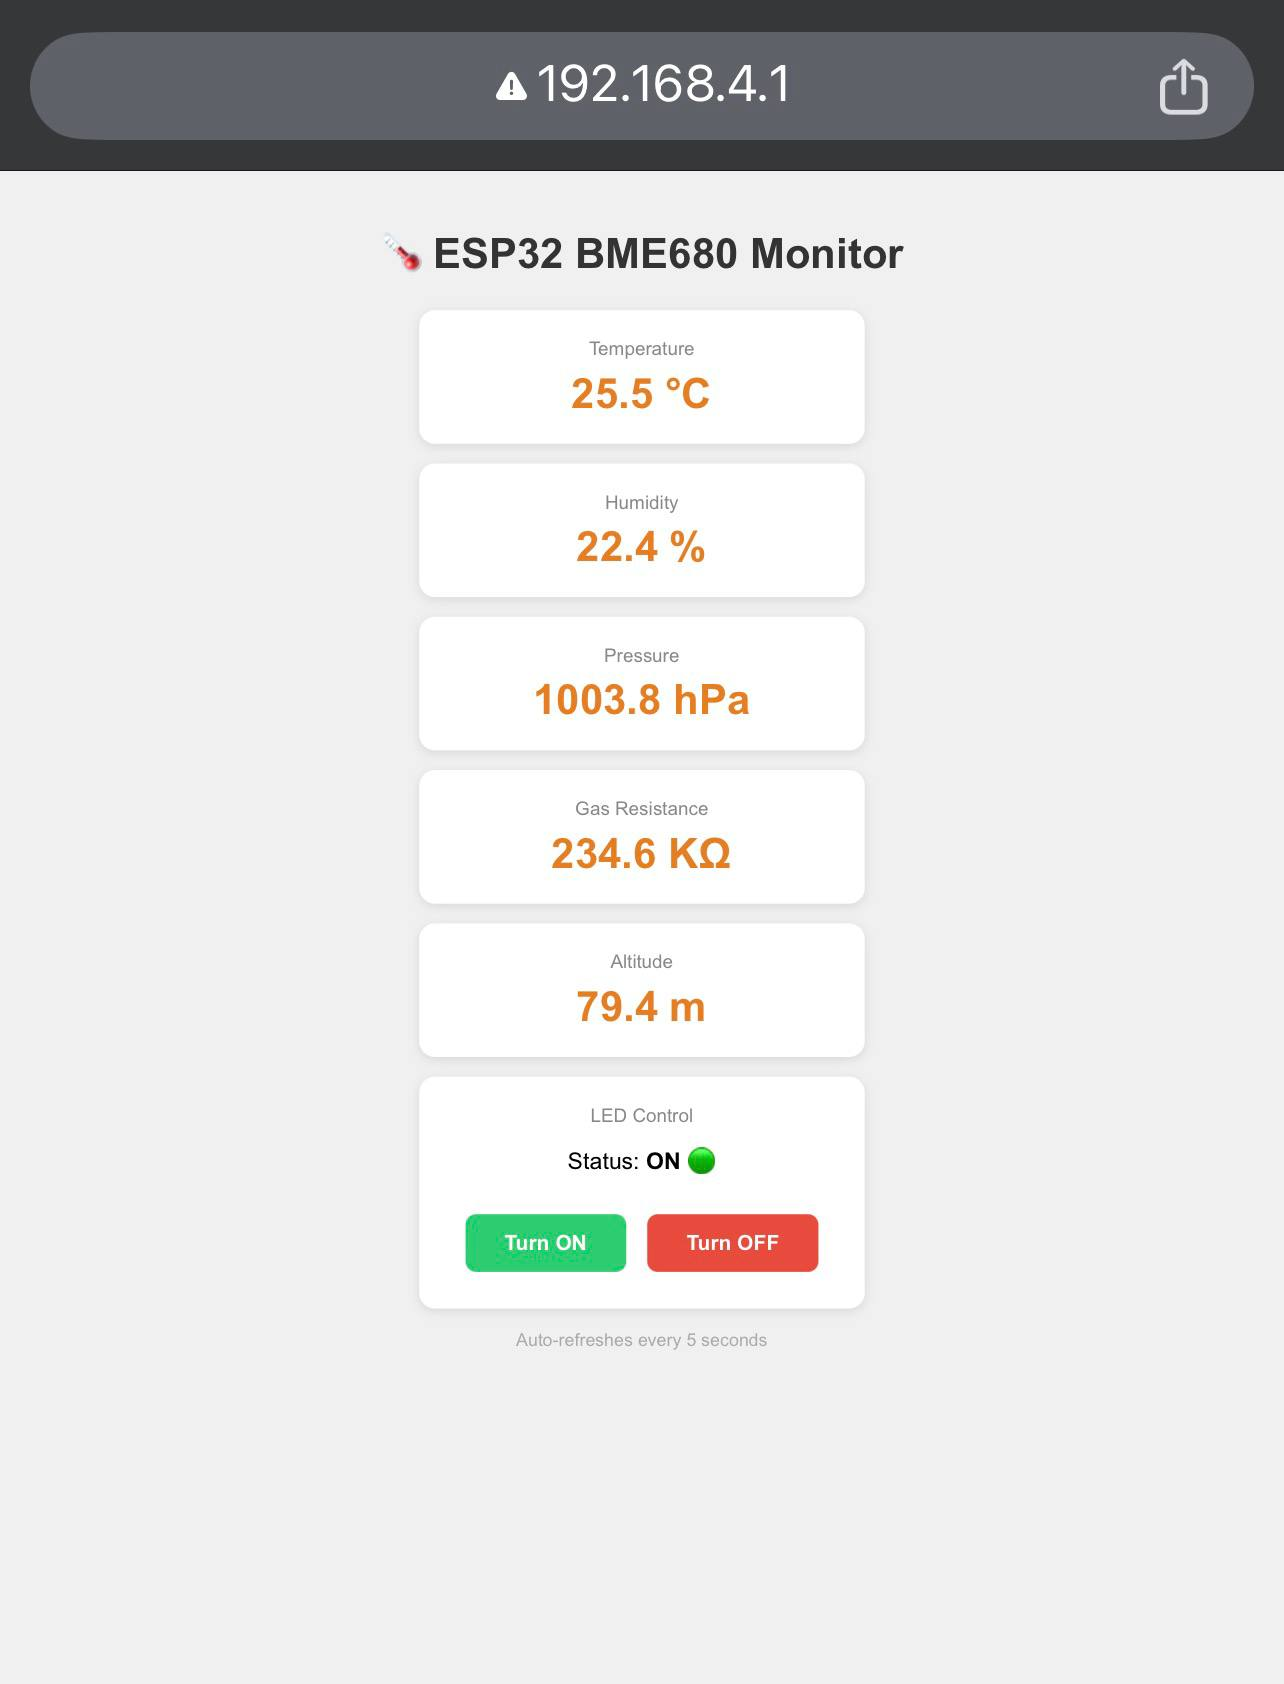
\includegraphics[width=\textwidth]{p1_dashboard_on.jpg}
        \caption{Dashboard with LED status ON.}
        \label{fig:p1_dashboard_on}
    \end{subfigure}
    \hfill
    \begin{subfigure}[b]{0.45\textwidth}
        \centering
        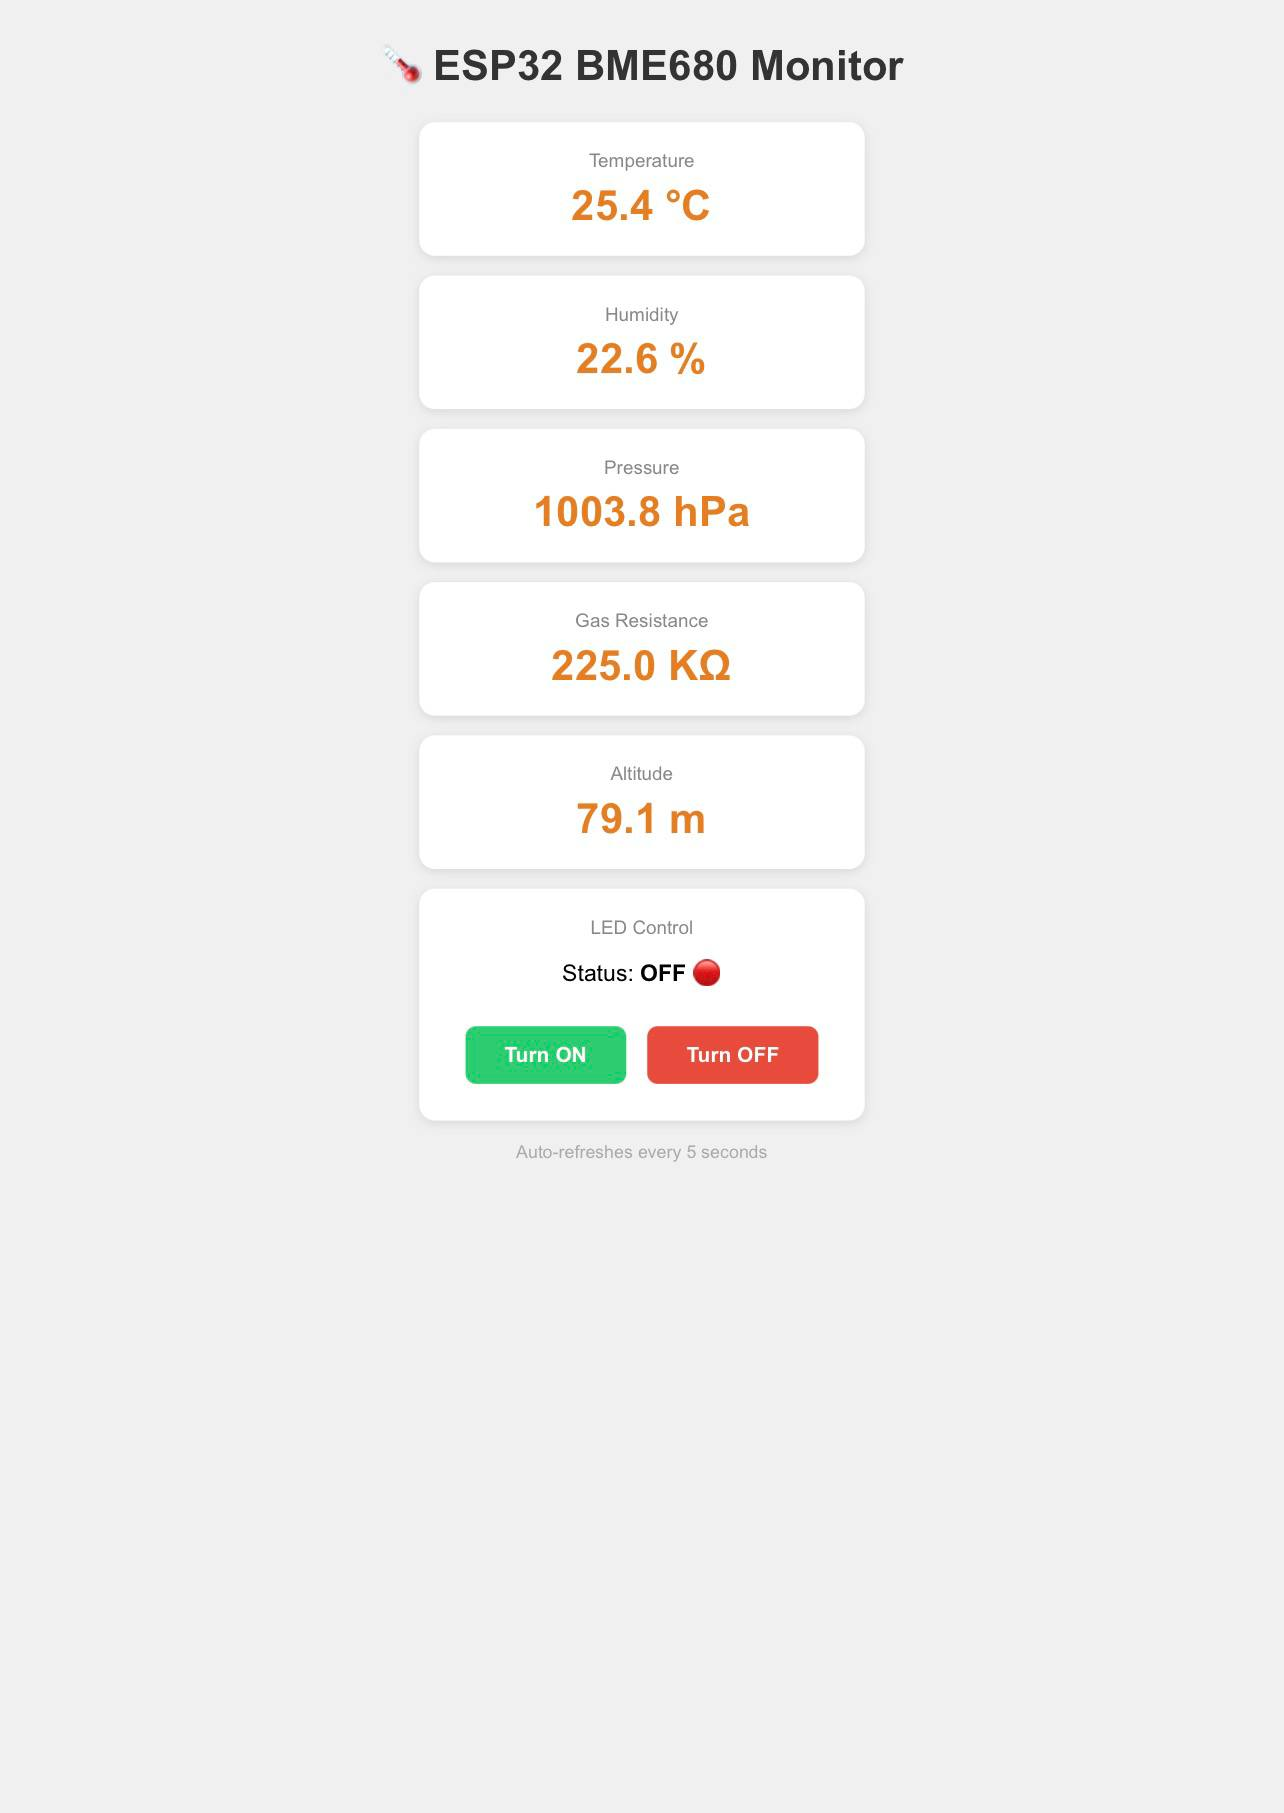
\includegraphics[width=\textwidth]{p1_dashboard_off.jpg}
        \caption{Dashboard with LED status OFF.}
        \label{fig:p1_dashboard_off}
    \end{subfigure}
    \caption{Sub-step 3: final web dashboard served by the ESP32, showing live BME680 readings and LED control.}
    \label{fig:p1_dashboard}
\end{figure}
 
\begin{figure}[H]
    \centering
    \begin{subfigure}[b]{0.45\textwidth}
        \centering
        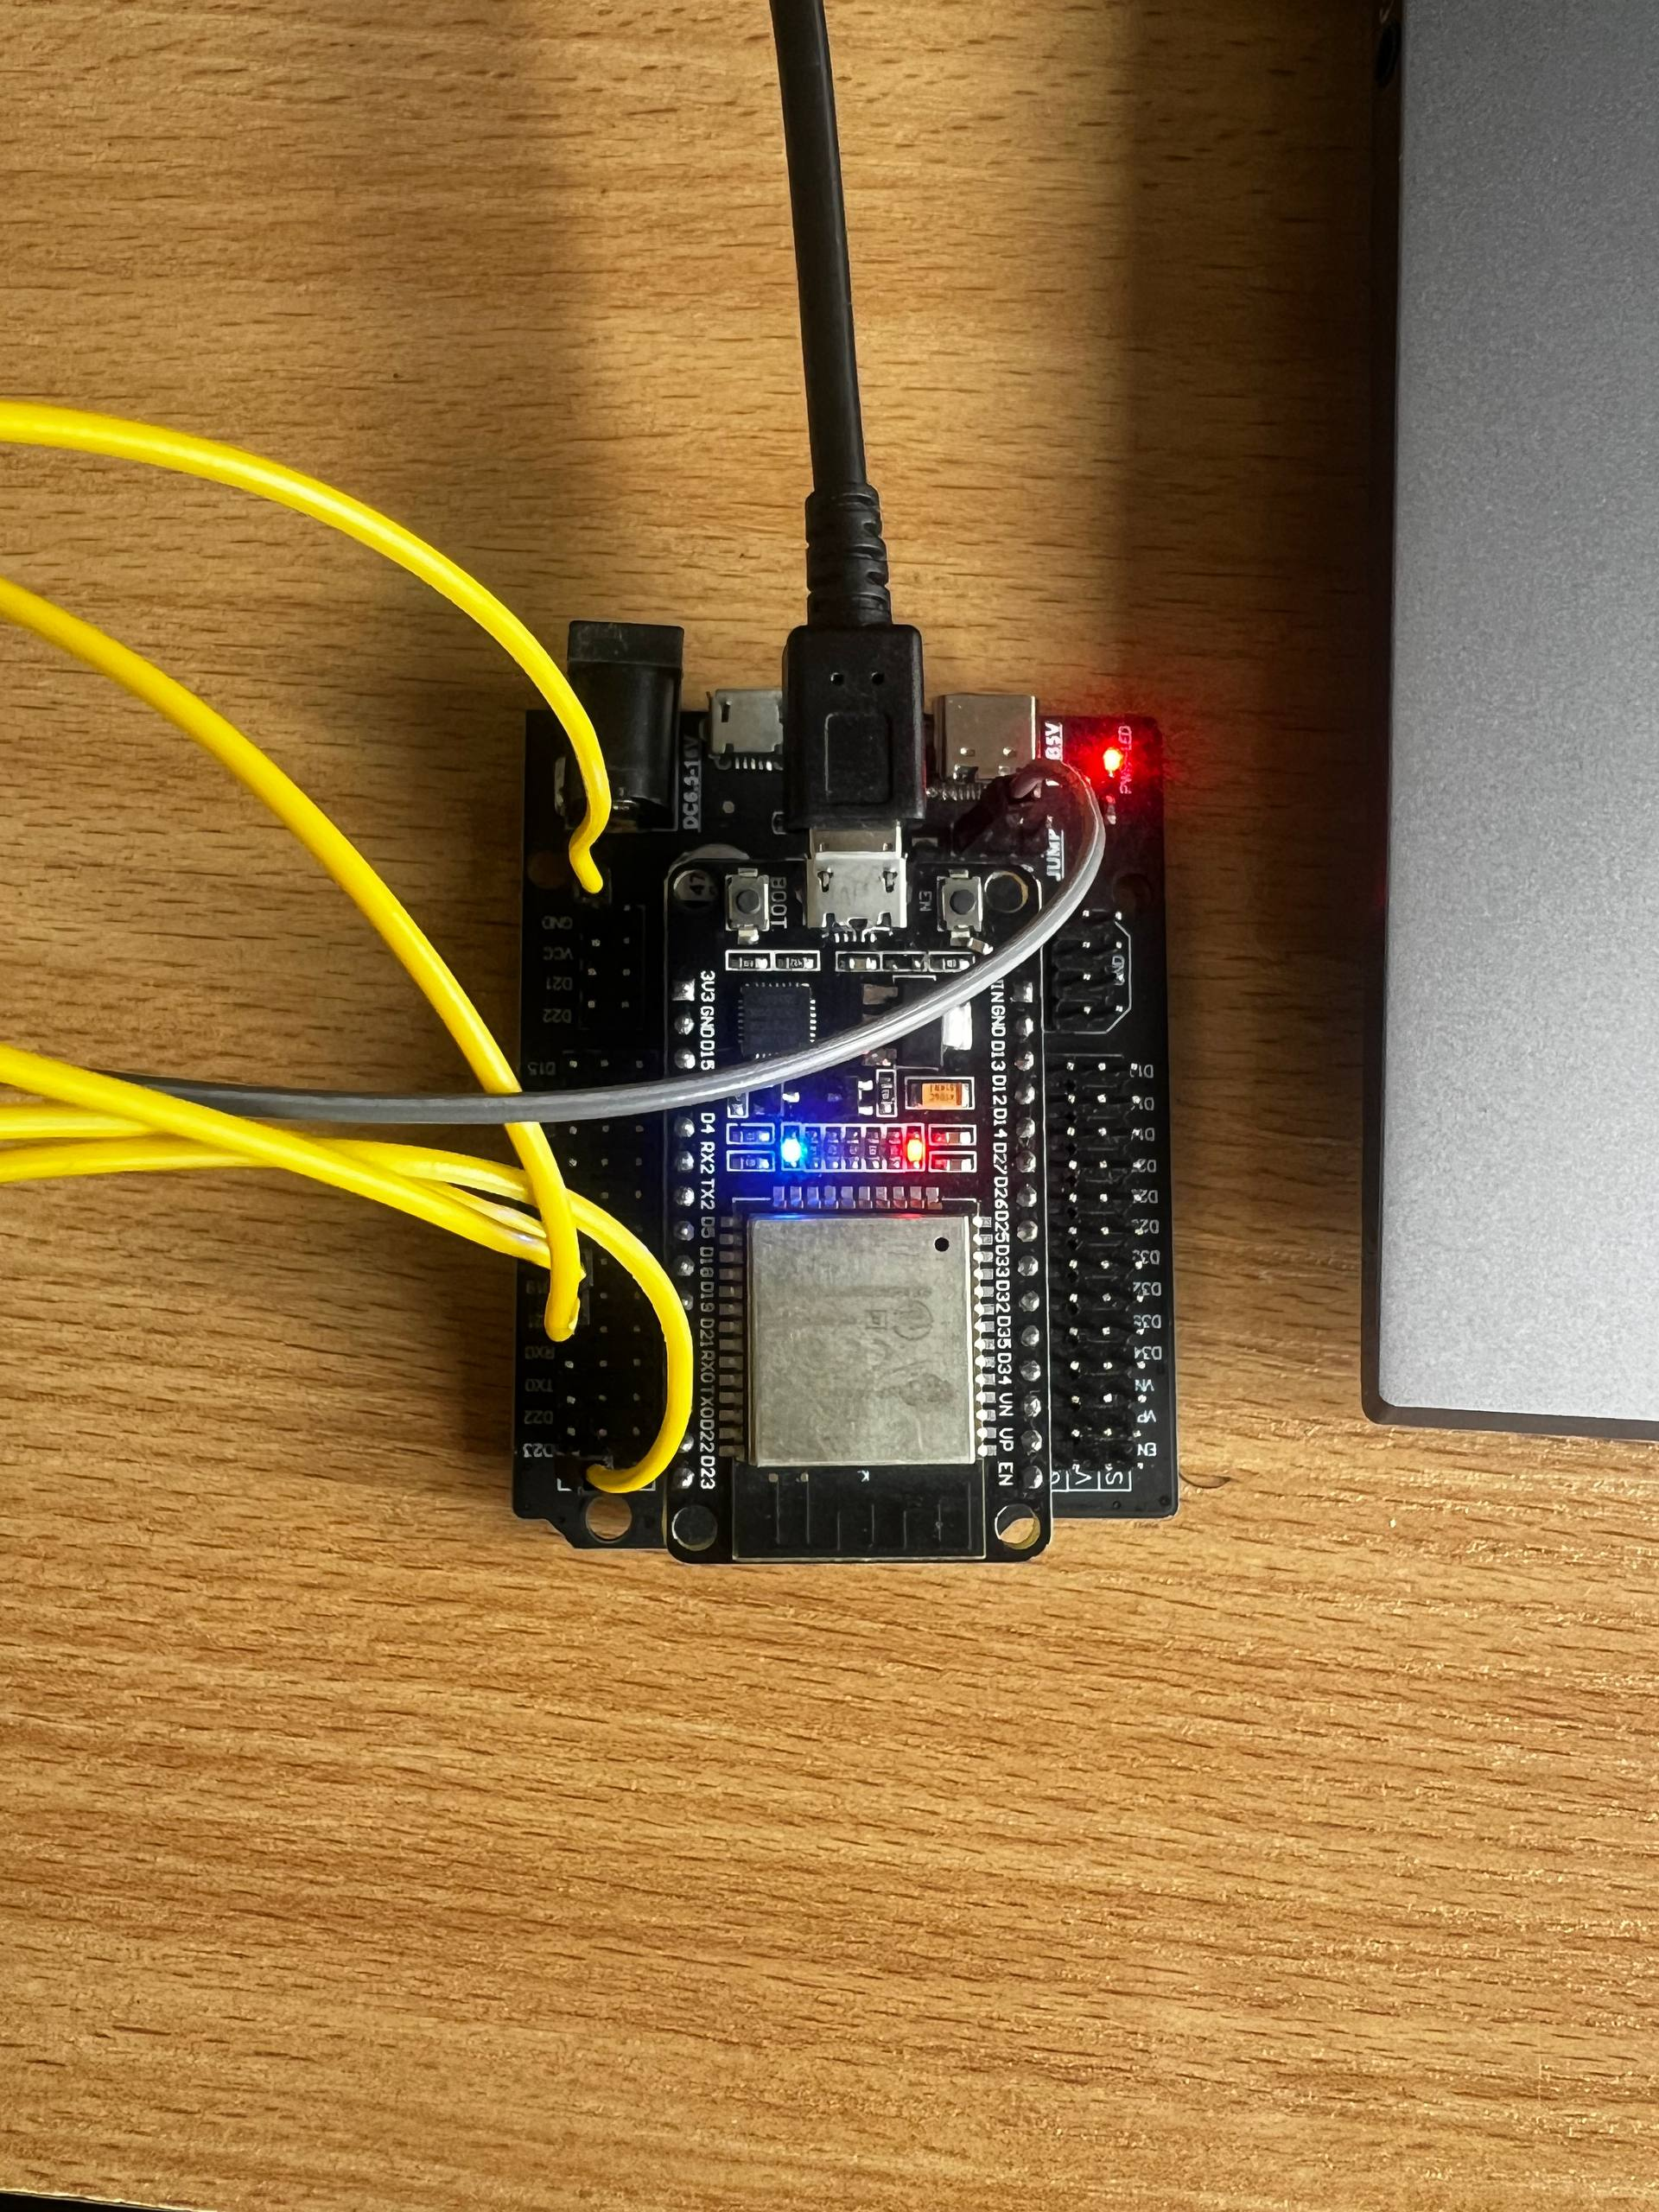
\includegraphics[width=\textwidth]{p1_led_on.jpg}
        \caption{ESP32 with LED ON (blue LED lit on pin~2).}
        \label{fig:p1_led_on}
    \end{subfigure}
    \hfill
    \begin{subfigure}[b]{0.45\textwidth}
        \centering
        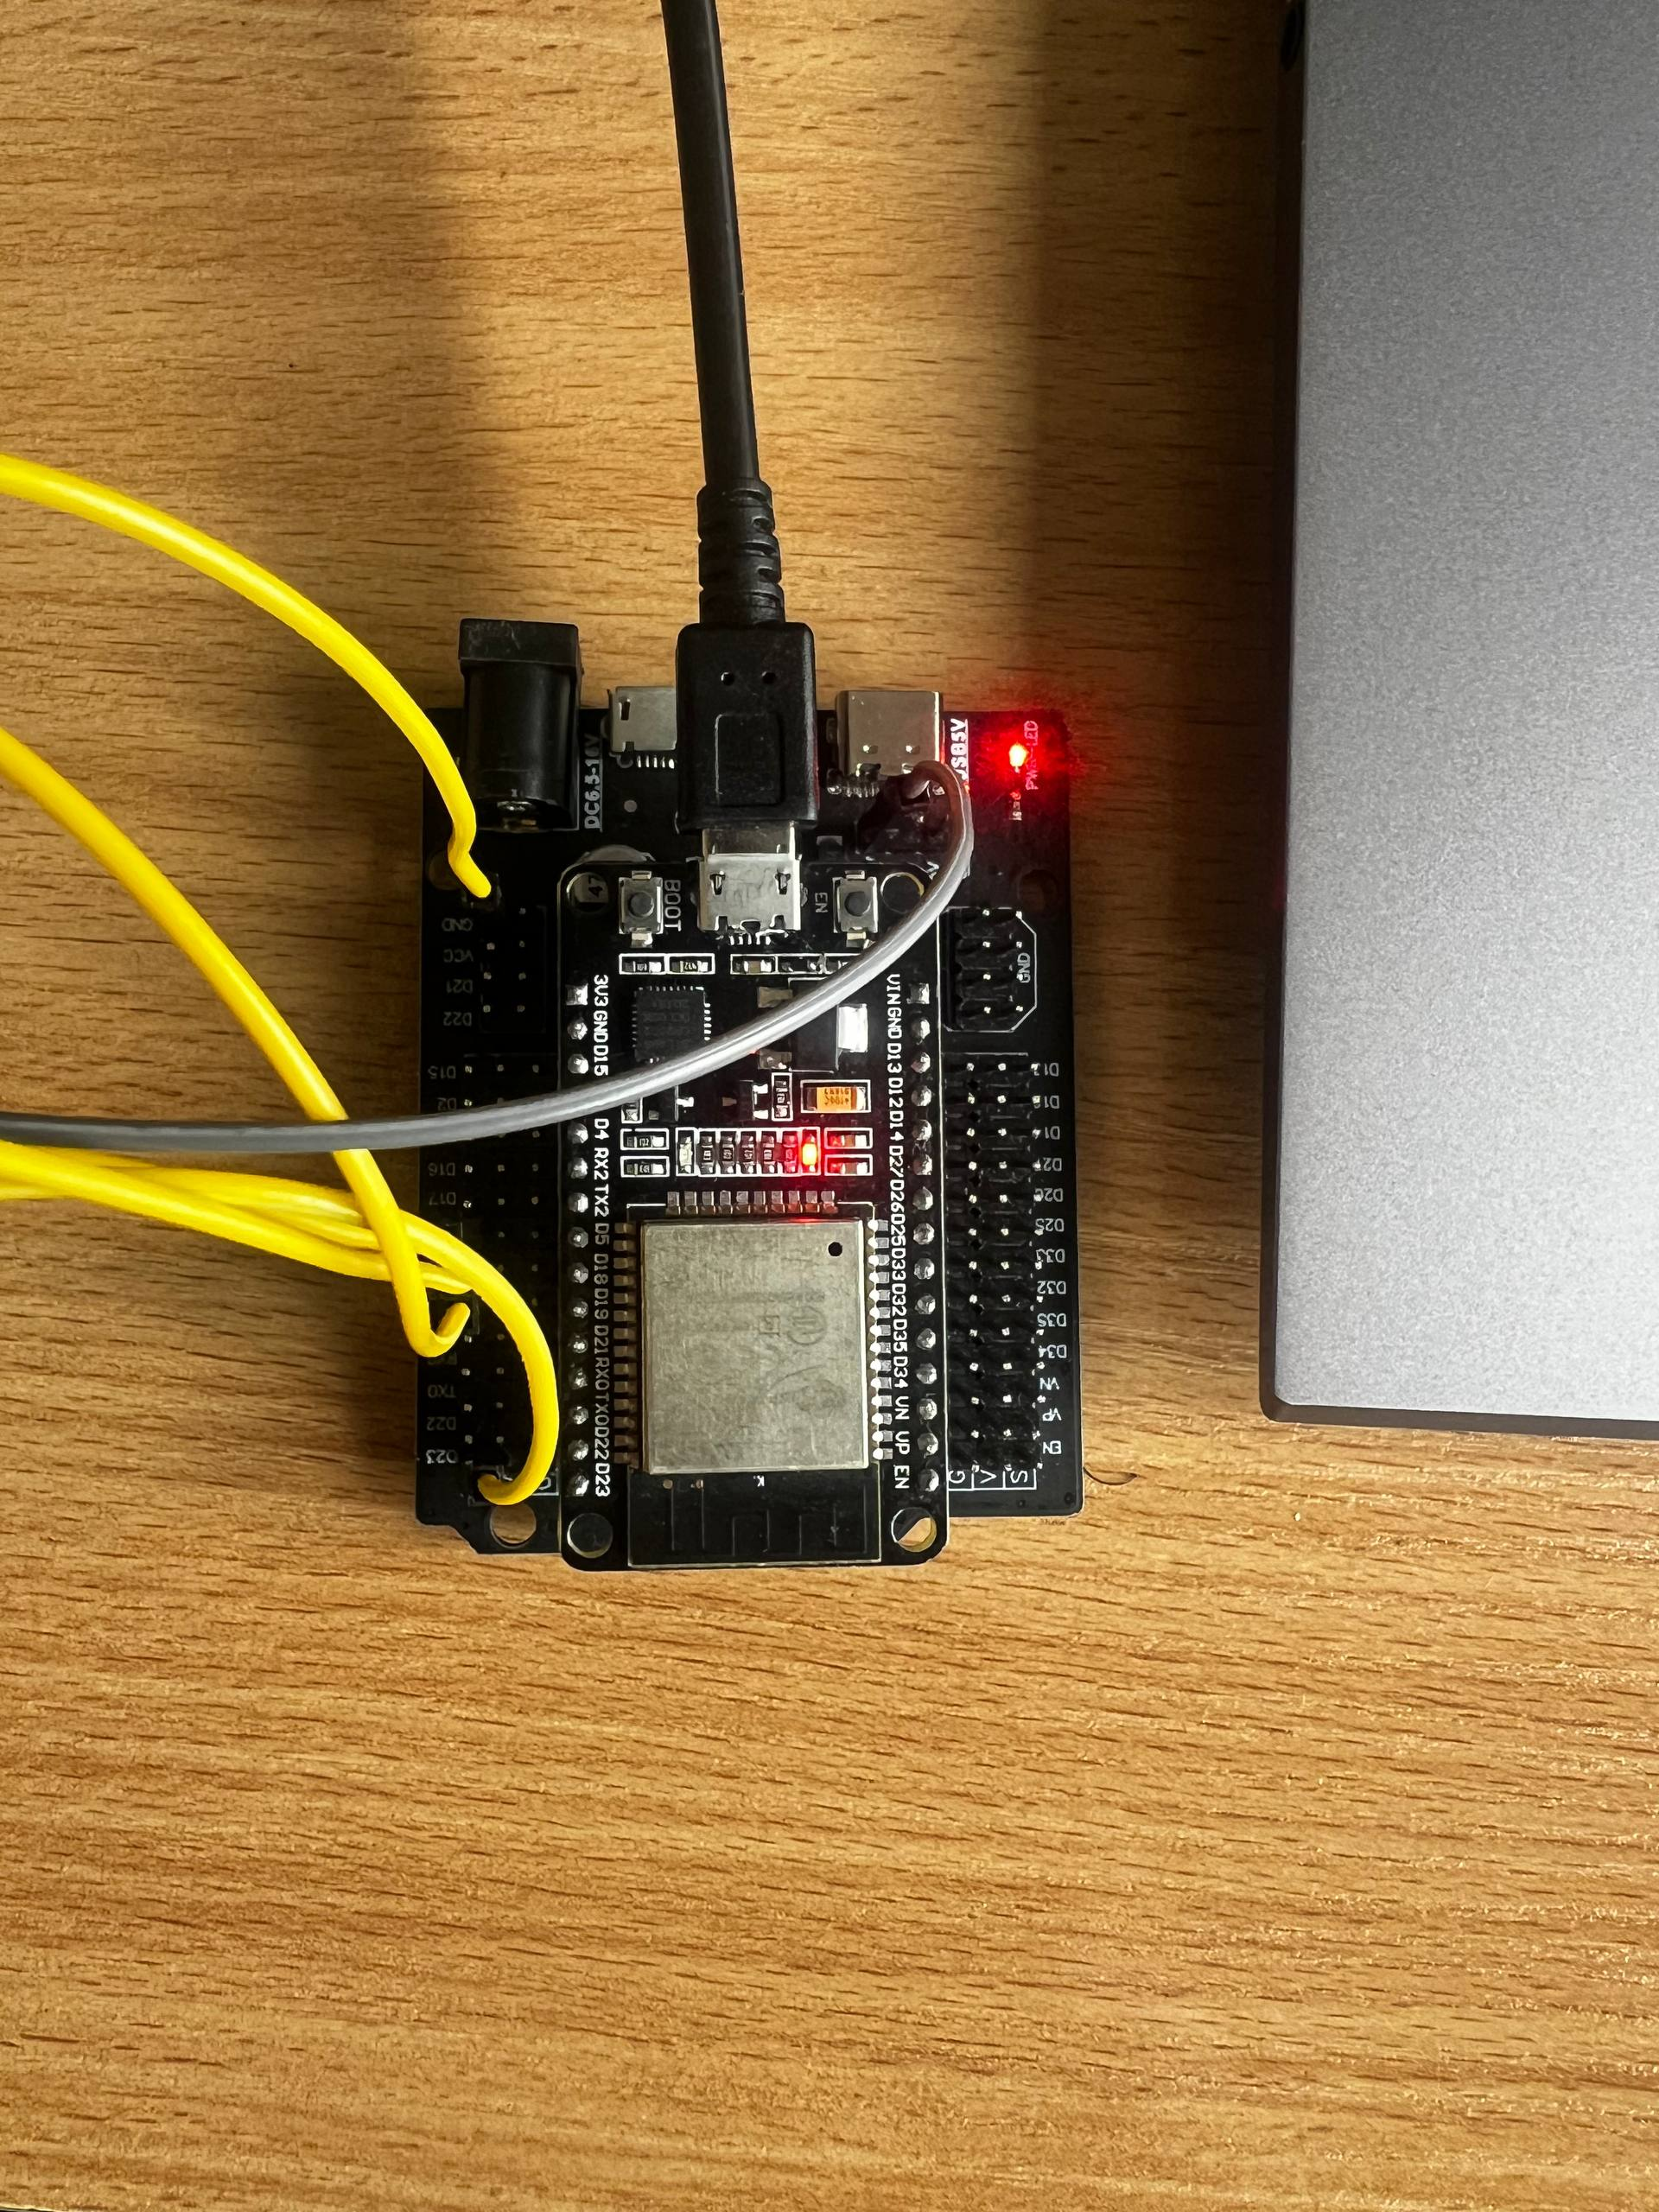
\includegraphics[width=\textwidth]{p1_led_off.jpg}
        \caption{ESP32 with LED OFF (only the power LED is lit).}
        \label{fig:p1_led_off}
    \end{subfigure}
    \caption{Hardware feedback on the ESP32 board, controlled from the web dashboard.}
    \label{fig:p1_led}
\end{figure}
 
The readings remained stable throughout the experiment, and the dashboard responded to button clicks within a few hundred milliseconds, confirming that the ESP32 is more than capable of handling the combined task of sensor sampling and HTTP serving.
 
%==================================================================
\chapter{Part 2 -- Gateway with Raspberry Pi and MQTT Broker}
%==================================================================
 
\section{Equipment and Libraries}
The gateway is built using the following components:
\begin{itemize}
    \item Raspberry Pi single-board computer with microSD card.
    \item Power supply, HDMI cable, monitor, keyboard and mouse.
    \item Ethernet cable or Wi-Fi connection to the local router.
    \item Raspberry Pi OS (clean installation prepared with Raspberry Pi Imager).
    \item Mosquitto MQTT broker and \texttt{mosquitto-clients} command-line tools.
\end{itemize}
 
\begin{figure}[H]
    \centering
    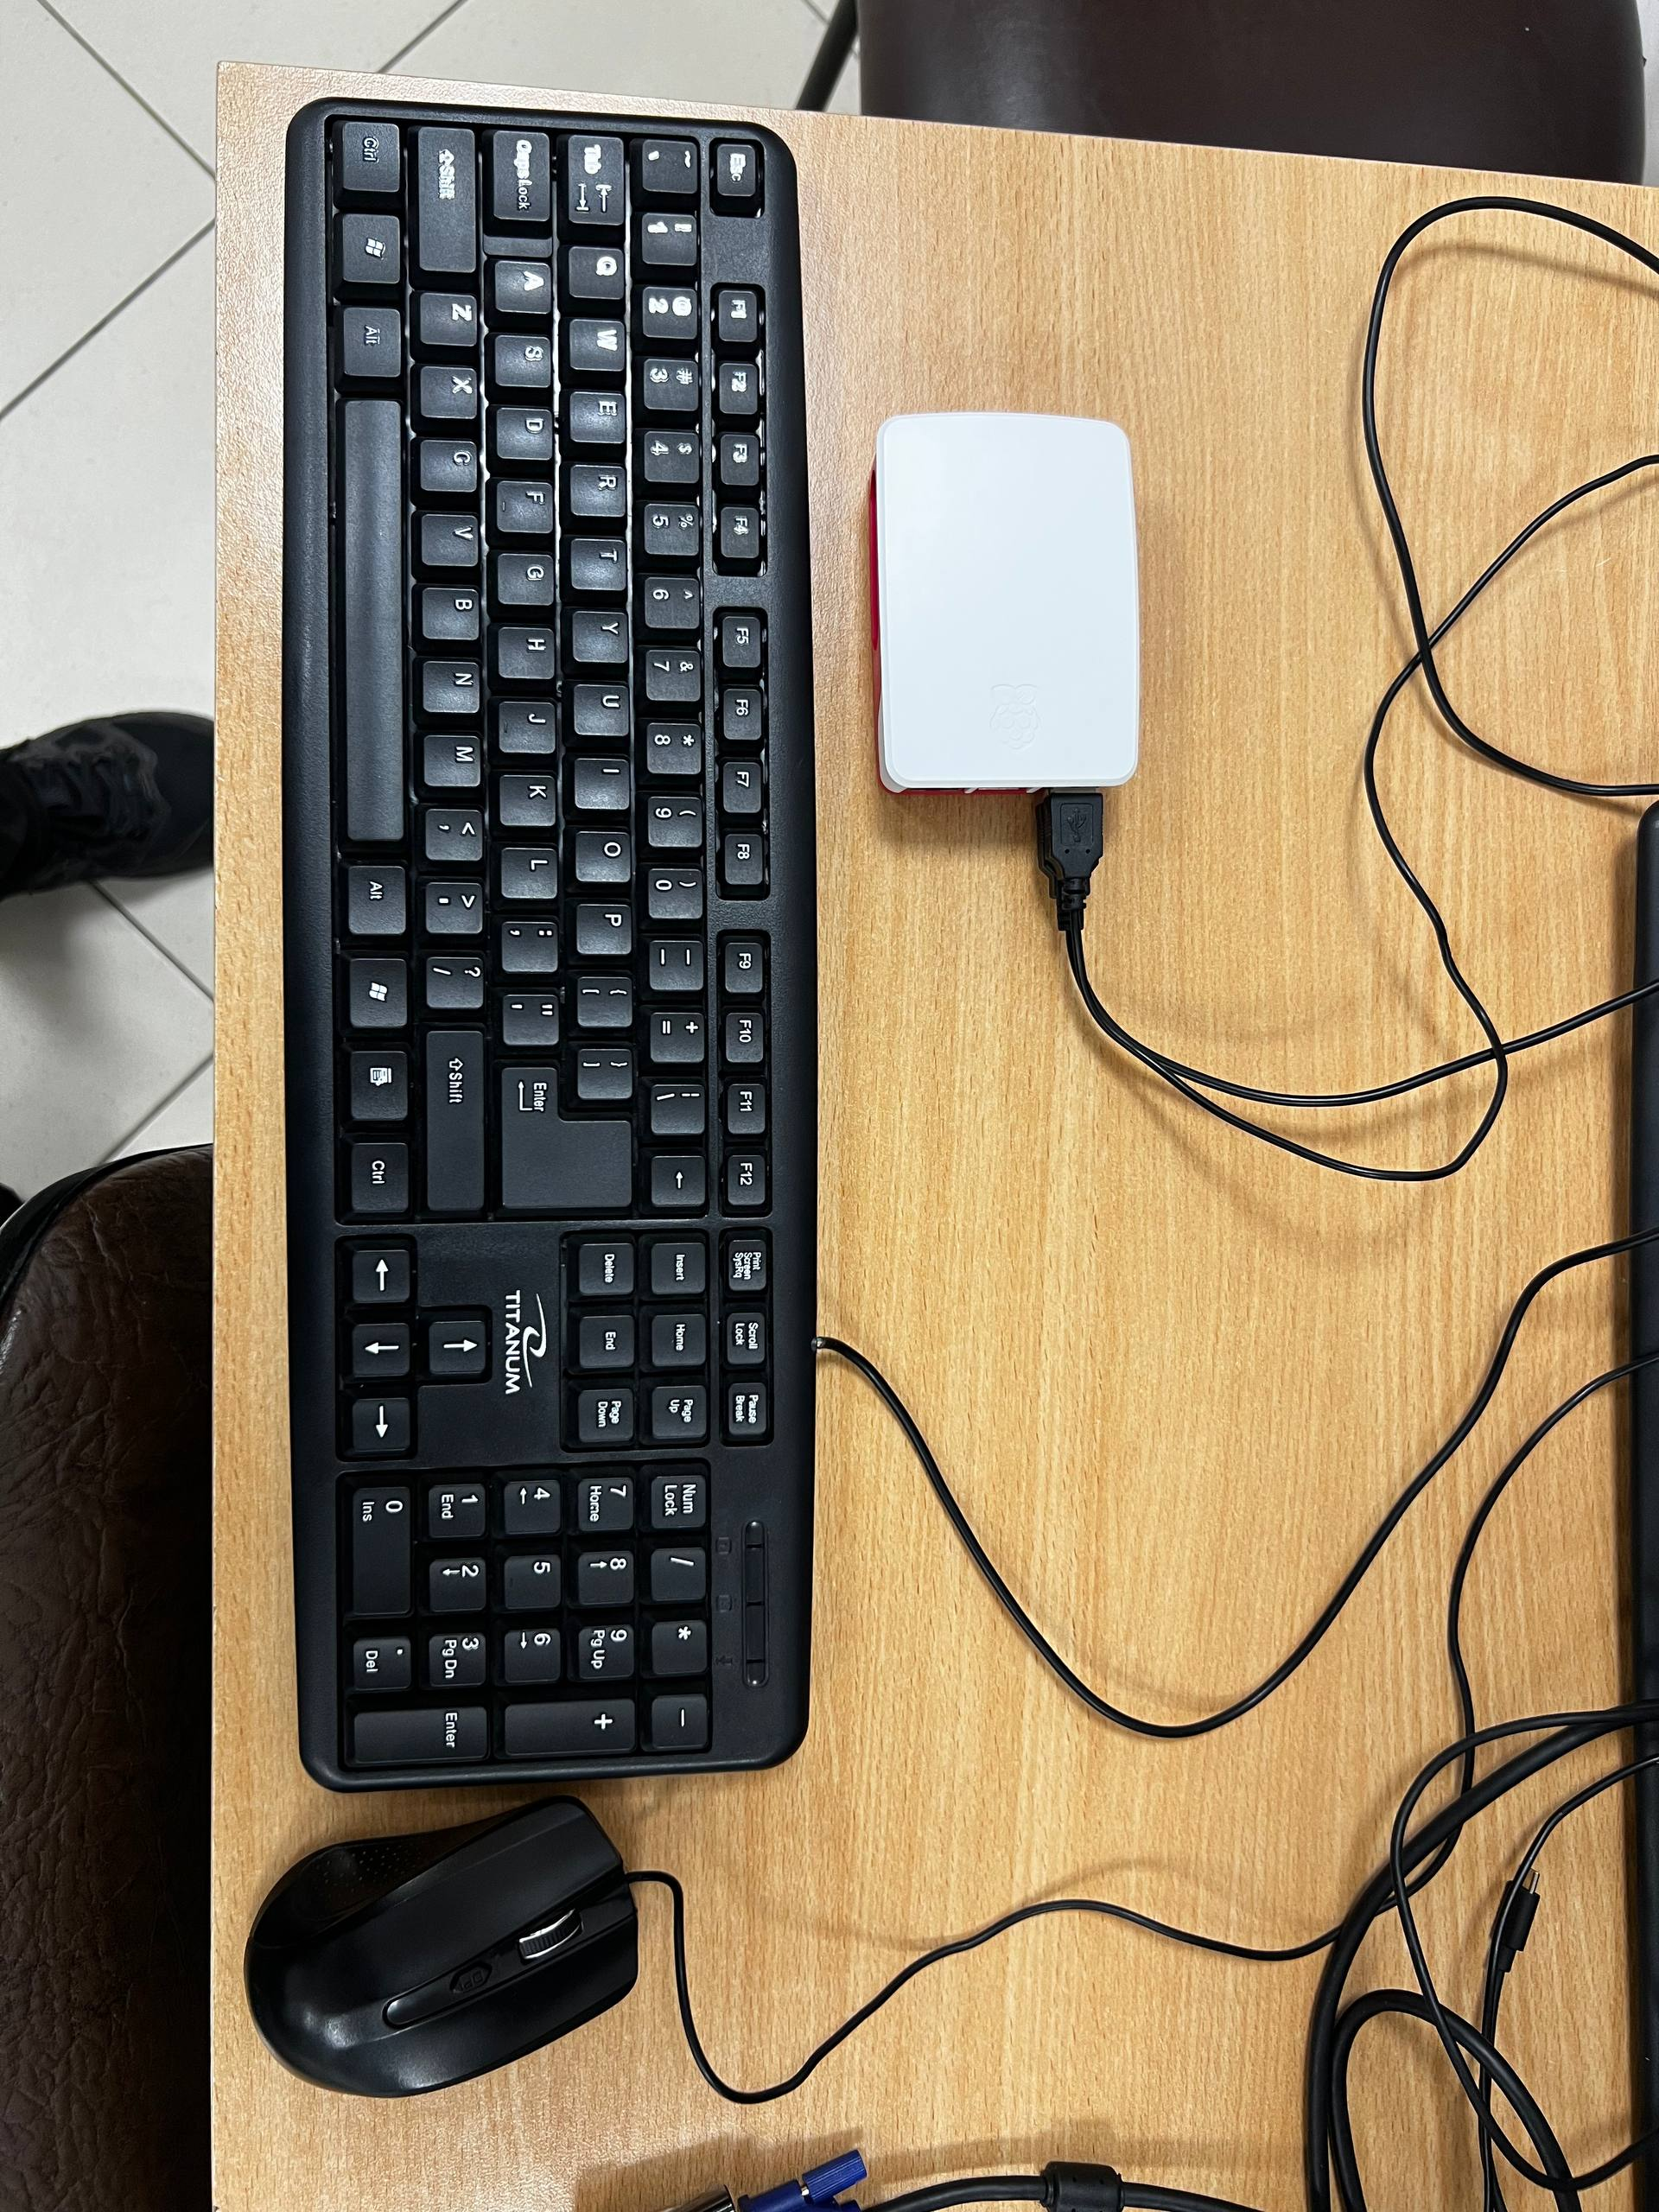
\includegraphics[width=0.7\textwidth, angle=90]{images/p2_rpi_case.jpg}
    \caption{Raspberry Pi Full Setup}
    \label{fig:p2_rpi_case}
\end{figure}
 
\section{Operating System Preparation}
 
The first step in building the gateway was to prepare a clean installation of Raspberry Pi OS using the official \emph{Raspberry Pi Imager} tool, downloaded from the Raspberry Pi website (Figure~\ref{fig:p2_imager_site}). During the configuration step of the Imager, the username \texttt{pi}, the password \texttt{raspberry} and the SSH access were set in advance, so that the Pi could be reached remotely after the first boot (We still programmed from inside the Raspberry Pi interface). The disk image was then written to the microSD card (Figure~\ref{fig:p2_imager_writing}).
 
\begin{figure}[H]
    \centering
    \begin{subfigure}[b]{0.48\textwidth}
        \centering
        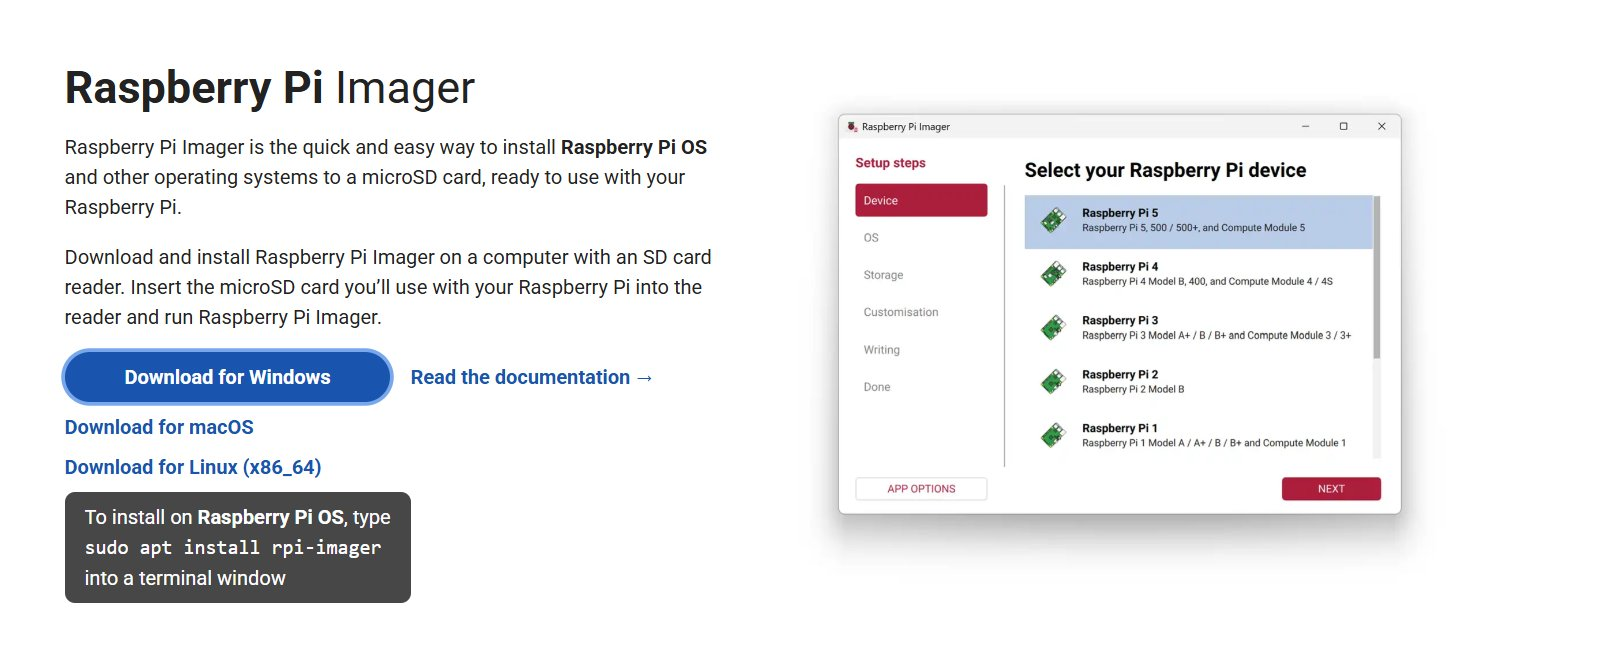
\includegraphics[width=\textwidth]{p2_imager_site.png}
        \caption{Raspberry Pi Imager download page.}
        \label{fig:p2_imager_site}
    \end{subfigure}
    \hfill
    \begin{subfigure}[b]{0.48\textwidth}
        \centering
        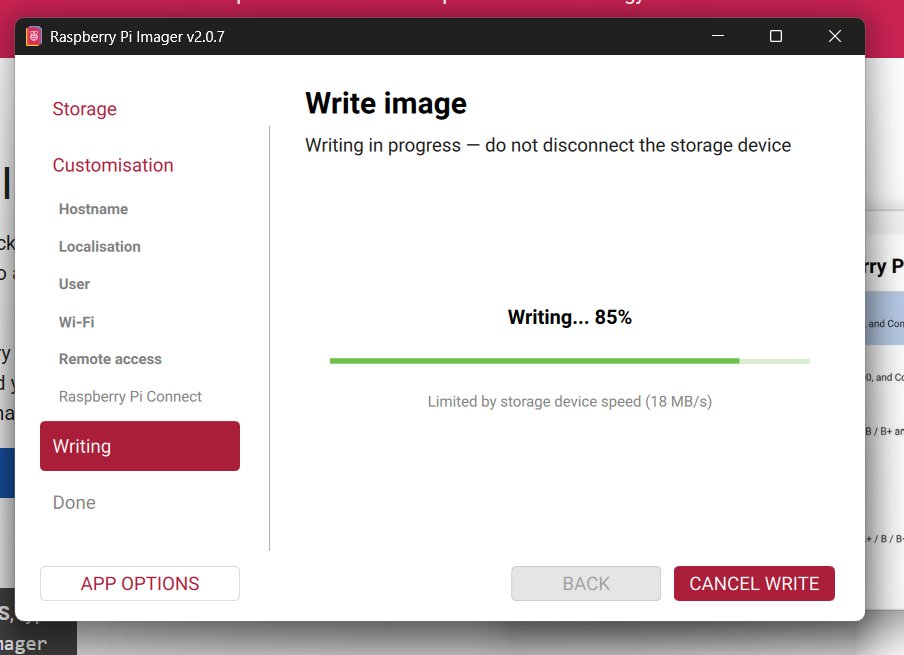
\includegraphics[width=\textwidth]{p2_imager_writing.png}
        \caption{Imager flashing the microSD card.}
        \label{fig:p2_imager_writing}
    \end{subfigure}
    \caption{Preparation of the Raspberry Pi OS installation through Raspberry Pi Imager.}
    \label{fig:p2_setup}
\end{figure}
 
\section{First Boot and \texttt{raspi-config}}
 
After inserting the microSD card and powering the Raspberry Pi, the system was further configured through the \texttt{raspi-config} utility, which allows the user to change low-level settings such as locale, timezone, interfaces and boot behaviour. In particular, the device was configured to boot to the text console (System Options $\to$ Boot / Auto Login $\to$ Console) as required by the laboratory specification.
 
\begin{figure}[H]
    \centering
    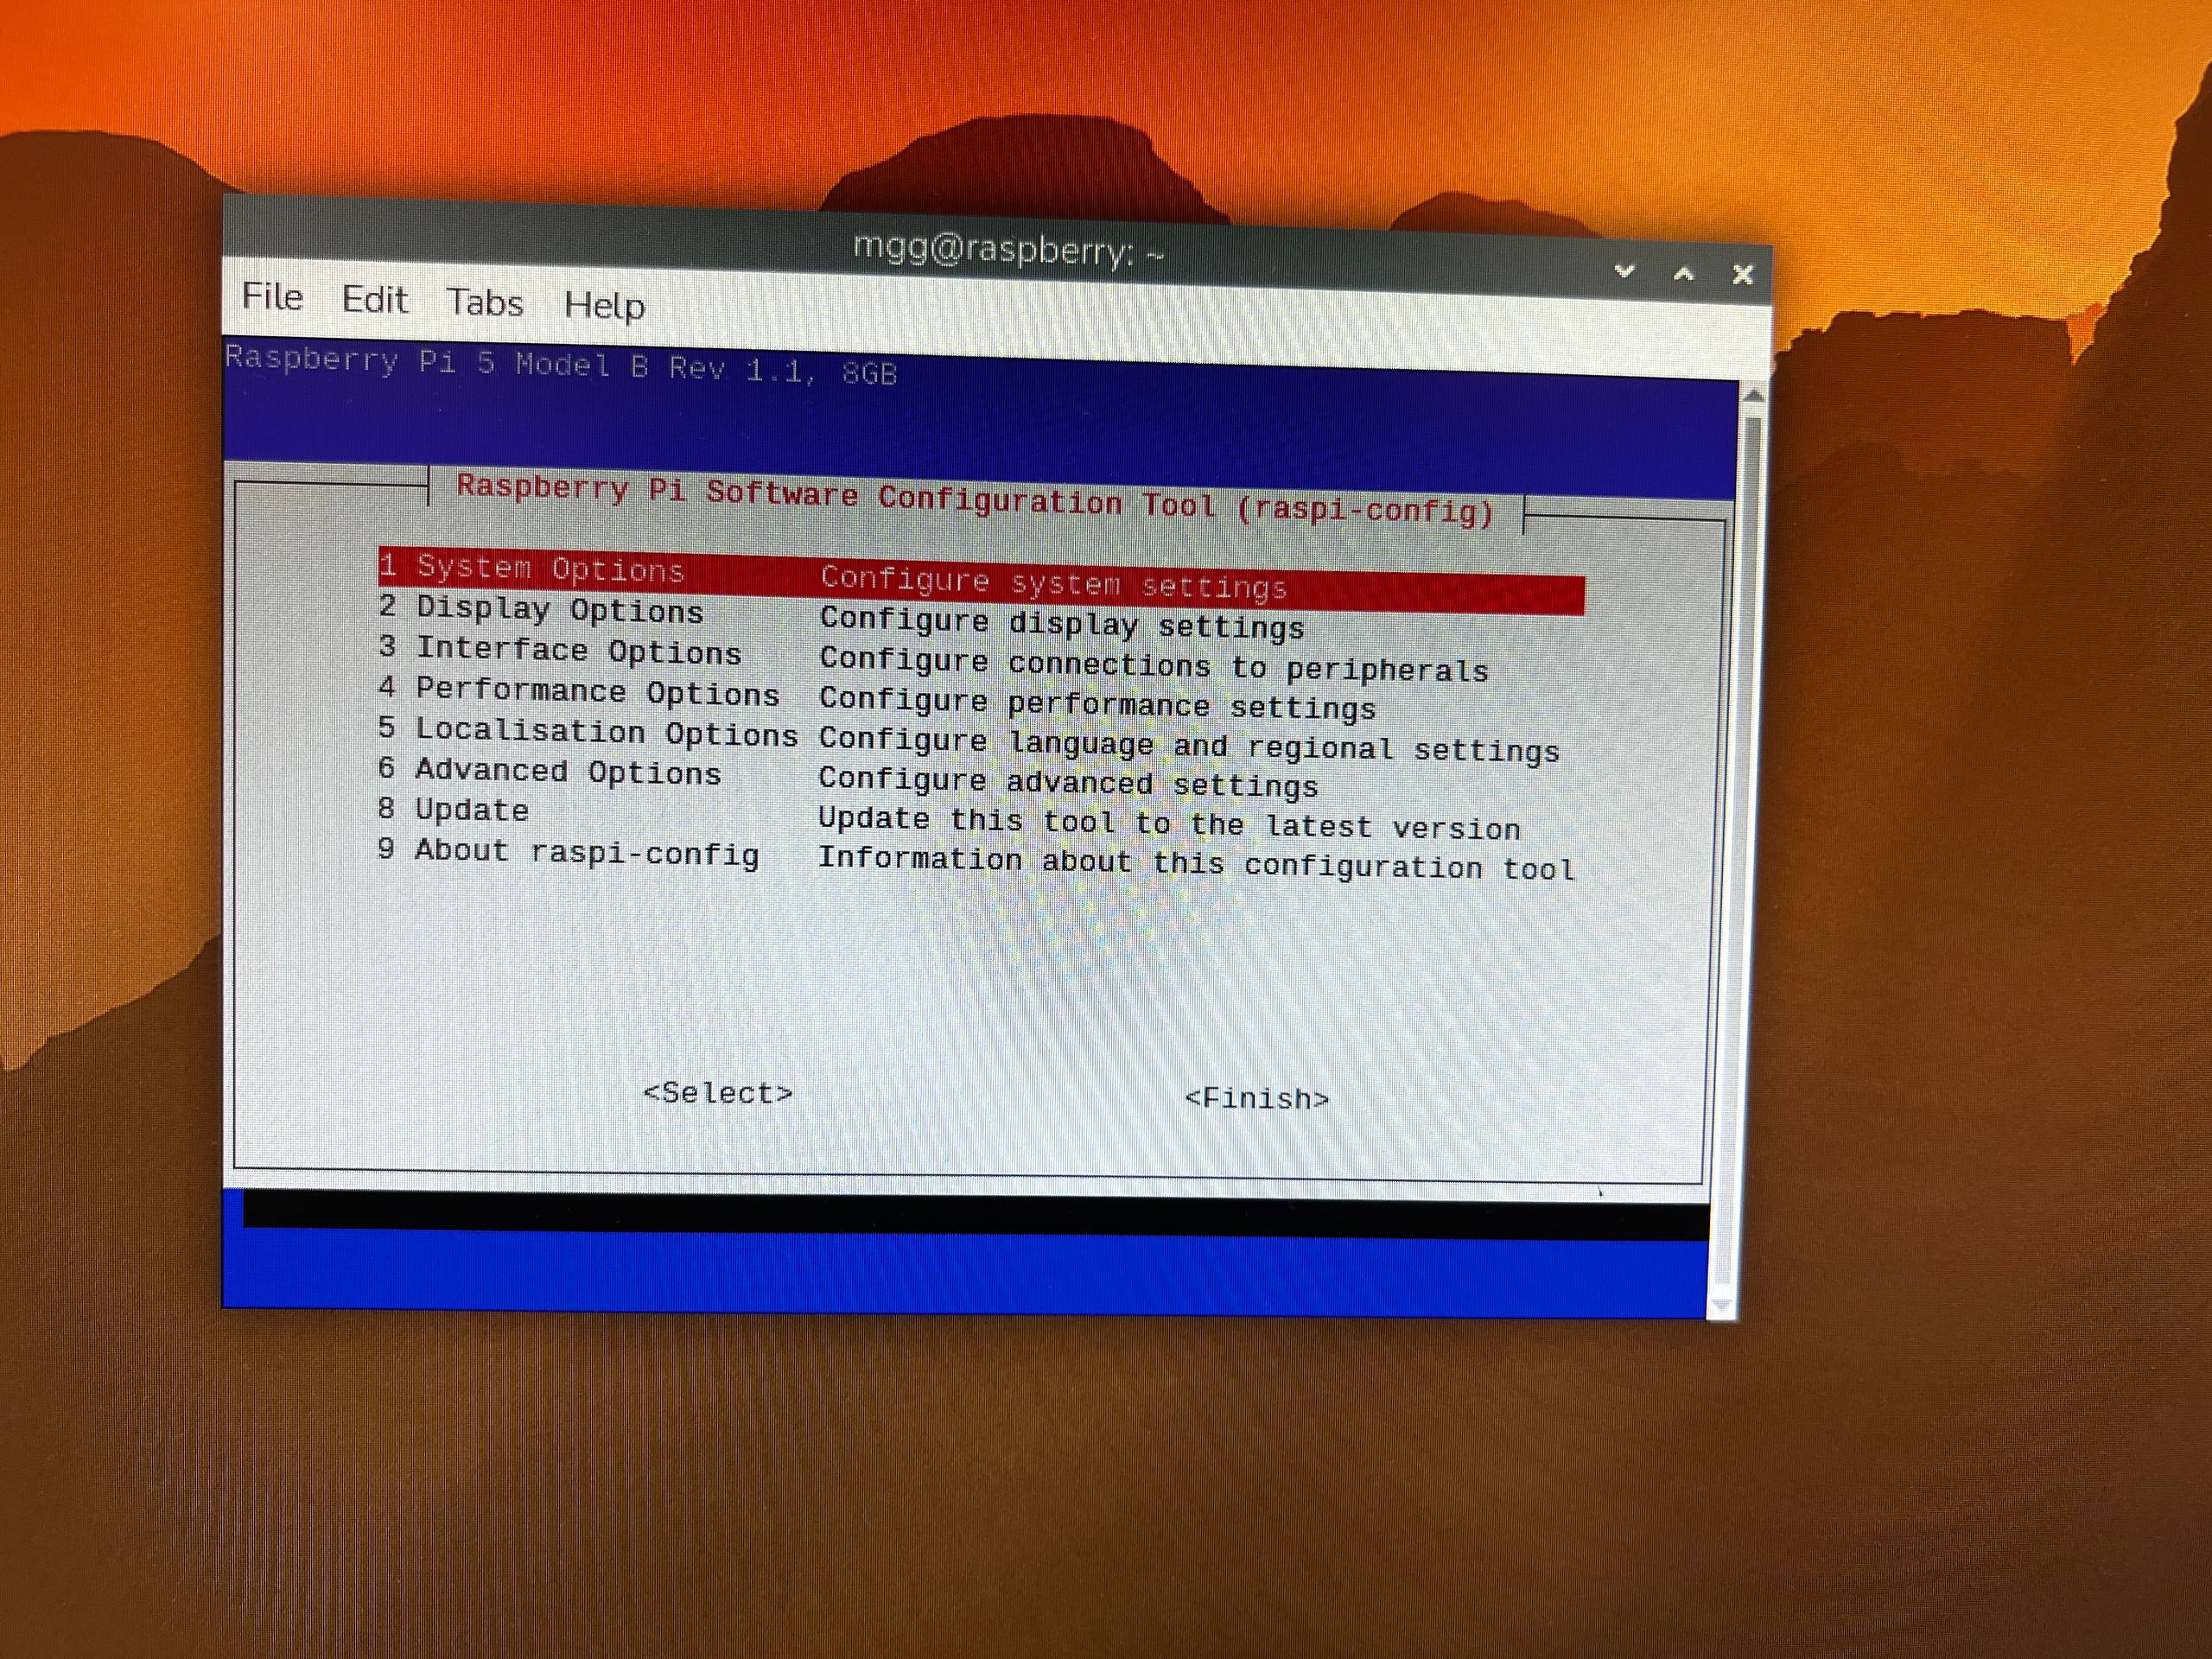
\includegraphics[width=0.8\textwidth]{p2_raspi_config.jpg}
    \caption{The \texttt{raspi-config} utility used to finalize the Raspberry Pi setup after the first boot.}
    \label{fig:p2_raspi_config}
\end{figure}
 
\section{Mosquitto Installation and Test}
 
Once the operating system was up and running, the \texttt{mosquitto} broker and the command-line clients (\texttt{mosquitto-clients}) were installed from the official Raspberry Pi OS package repositories. The broker was then enabled to start automatically at boot, and a basic publish/subscribe test was performed locally on the Pi using two terminals: one running \texttt{mosquitto\_sub} (subscribed to the topic \texttt{class/test}) and the other running \texttt{mosquitto\_pub} (publishing the message \texttt{"Hello world!"} to the same topic). The relevant commands are reported below.
 
\begin{lstlisting}[language=bash, caption={Mosquitto installation and basic test commands.}]
# Update package lists and install Mosquitto broker + clients
sudo apt update
sudo apt install mosquitto mosquitto-clients
 
# Enable Mosquitto to start automatically at boot
sudo systemctl enable mosquitto
sudo systemctl start mosquitto
 
# Check the broker status
sudo systemctl status mosquitto
 
# Subscribe to a test topic (terminal 1)
mosquitto_sub -h localhost -t class/test
 
# Publish a test message (terminal 2)
mosquitto_pub -h localhost -t class/test -m "Hello world!"
\end{lstlisting}
 
\section{Results}
 
The publish/subscribe mechanism worked at the first attempt: the message published with \texttt{mosquitto\_pub} (Figure~\ref{fig:p2_mosquitto_pub}) was received instantly by the \texttt{mosquitto\_sub} client subscribed to the same topic, which printed it on the console (Figure~\ref{fig:p2_mosquitto_sub}). This local test confirmed that the broker was correctly installed, running and capable of routing messages.
 
\begin{figure}[H]
    \centering
    \begin{subfigure}[b]{0.48\textwidth}
        \centering
        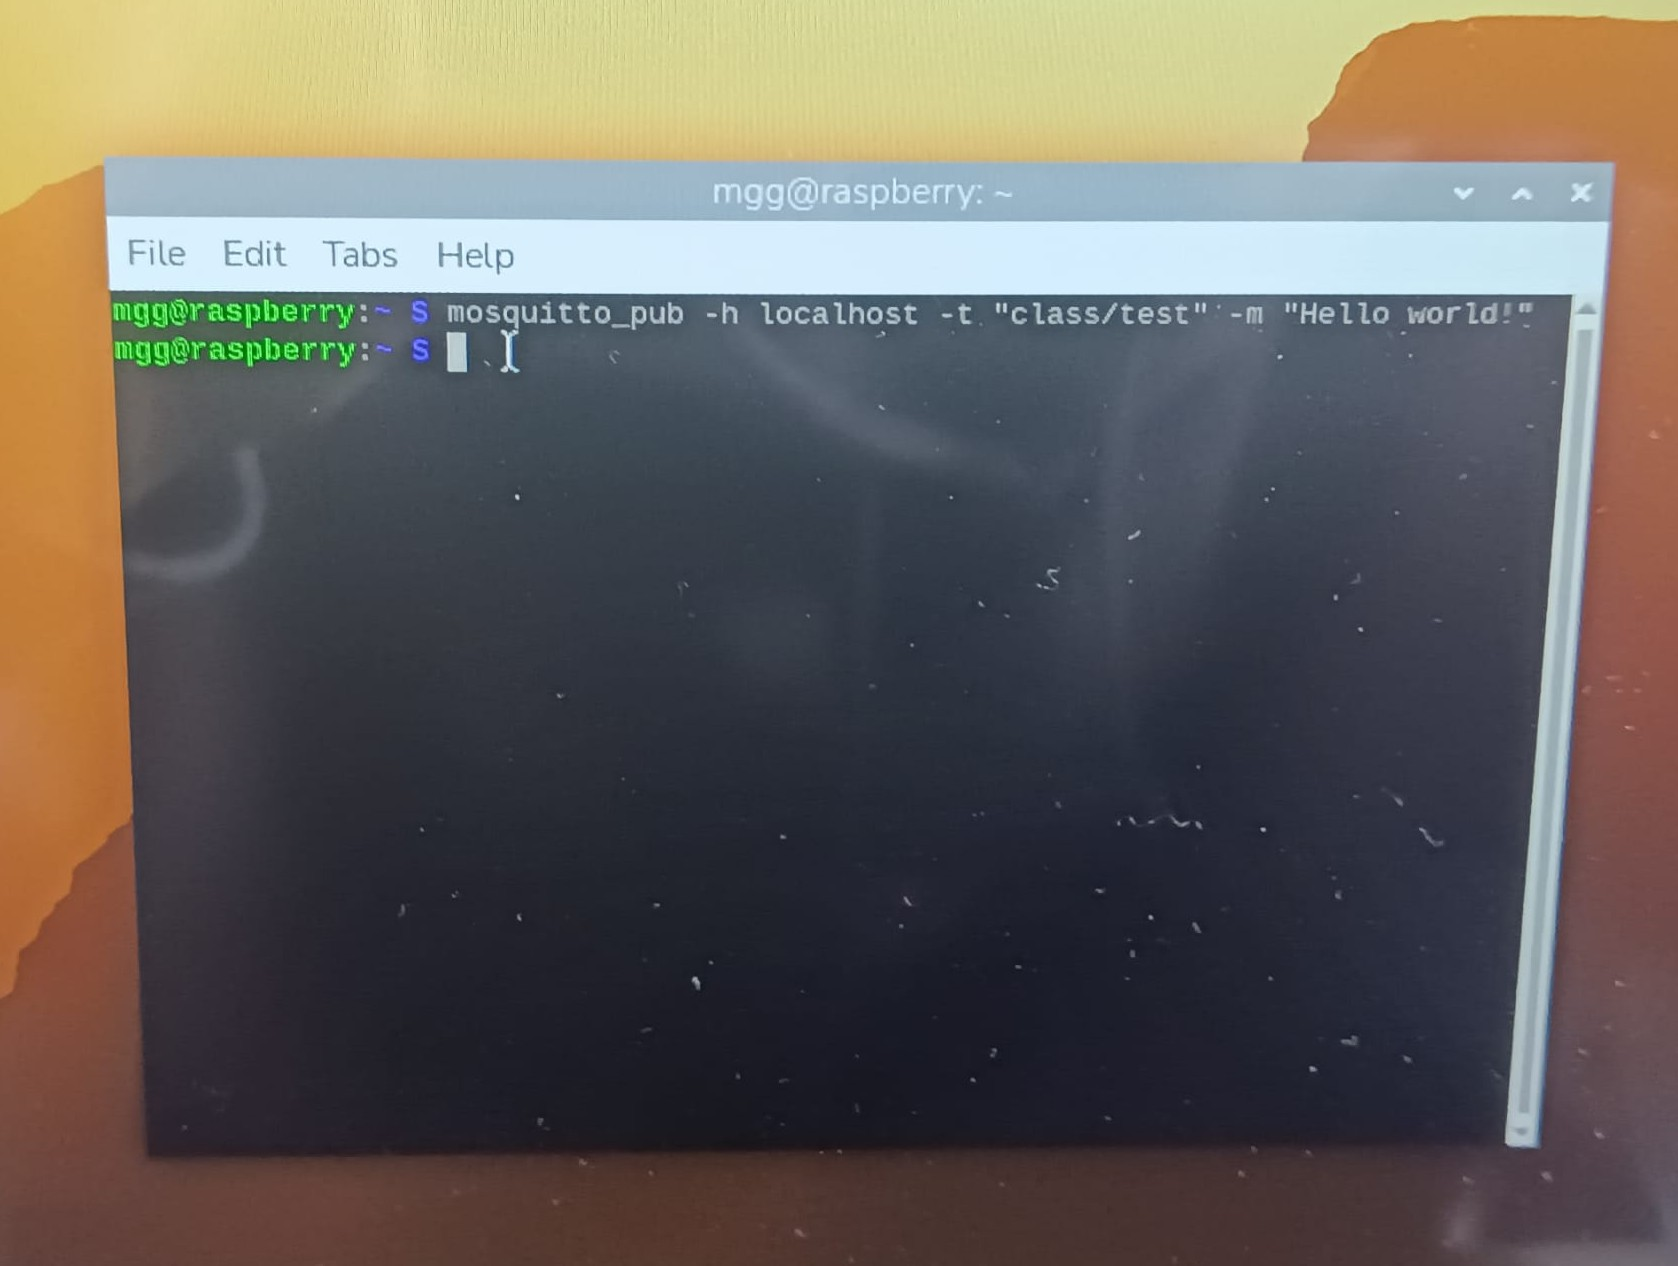
\includegraphics[width=\textwidth]{p2_mosquitto_pub.jpg}
        \caption{\texttt{mosquitto\_pub} publishing the test message.}
        \label{fig:p2_mosquitto_pub}
    \end{subfigure}
    \hfill
    \begin{subfigure}[b]{0.48\textwidth}
        \centering
        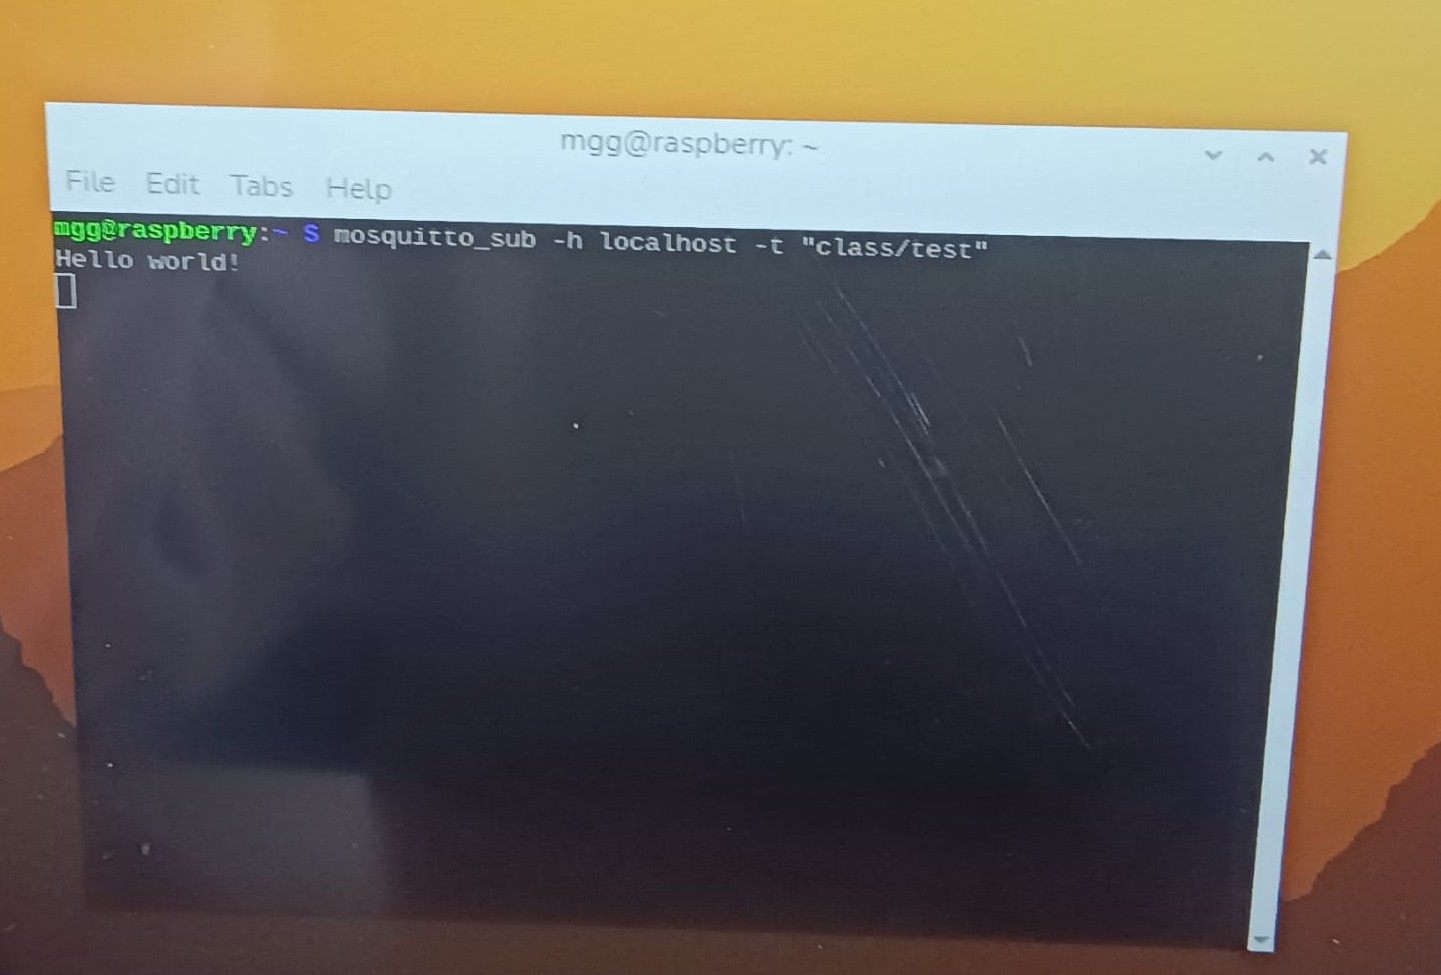
\includegraphics[width=\textwidth]{p2_mosquitto_sub.jpg}
        \caption{\texttt{mosquitto\_sub} receiving the message.}
        \label{fig:p2_mosquitto_sub}
    \end{subfigure}
    \caption{Local validation of the Mosquitto broker on the Raspberry Pi using the topic \texttt{class/test}.}
    \label{fig:p2_mqtt_test}
\end{figure}
 
%==================================================================
\chapter{Part 3 -- Complete IoT System Integration}
%==================================================================
 
\section{Equipment}
The third part combines the equipment used in the previous two parts:
\begin{itemize}
    \item ESP32 DevKit board with the BME680 sensor (from Part~1).
    \item Raspberry Pi running the Mosquitto MQTT broker (from Part~2).
    \item Wireless router providing the local Wi-Fi network.
    \item Personal computer for programming the ESP32 and accessing the Raspberry Pi.
    \item Arduino library \texttt{PubSubClient} for the MQTT client side on the ESP32.
\end{itemize}
 
The configuration requirements for this part are:
\begin{itemize}
    \item The Raspberry Pi must be connected to the wireless router.
    \item The MQTT broker on the Raspberry Pi must be running and accept connections from external devices.
    \item The MQTT client on the Raspberry Pi must subscribe to the topic \texttt{system/+/data} (or, more specifically, \texttt{system/1234/data}).
    \item The ESP32 must be connected to the same wireless router and to the broker on the Raspberry Pi.
    \item The ESP32 must publish messages to the topic \texttt{system/1234/data}, containing real BME680 sensor data formatted as a JSON object.
\end{itemize}
 
\section{Hardware Connections}
 
The wiring of the ESP32 and the BME680 sensor is identical to Part~1; the only difference at the hardware level is that the Raspberry Pi gateway is now part of the same Wi-Fi network as the ESP32. Figure~\ref{fig:p3_full_setup} shows the complete experimental setup with the Raspberry Pi (in its red/white case), the ESP32 + BME680 node on the breadboard, and the development workstation used to monitor both ends of the chain.
 
\begin{figure}[H]
    \centering
    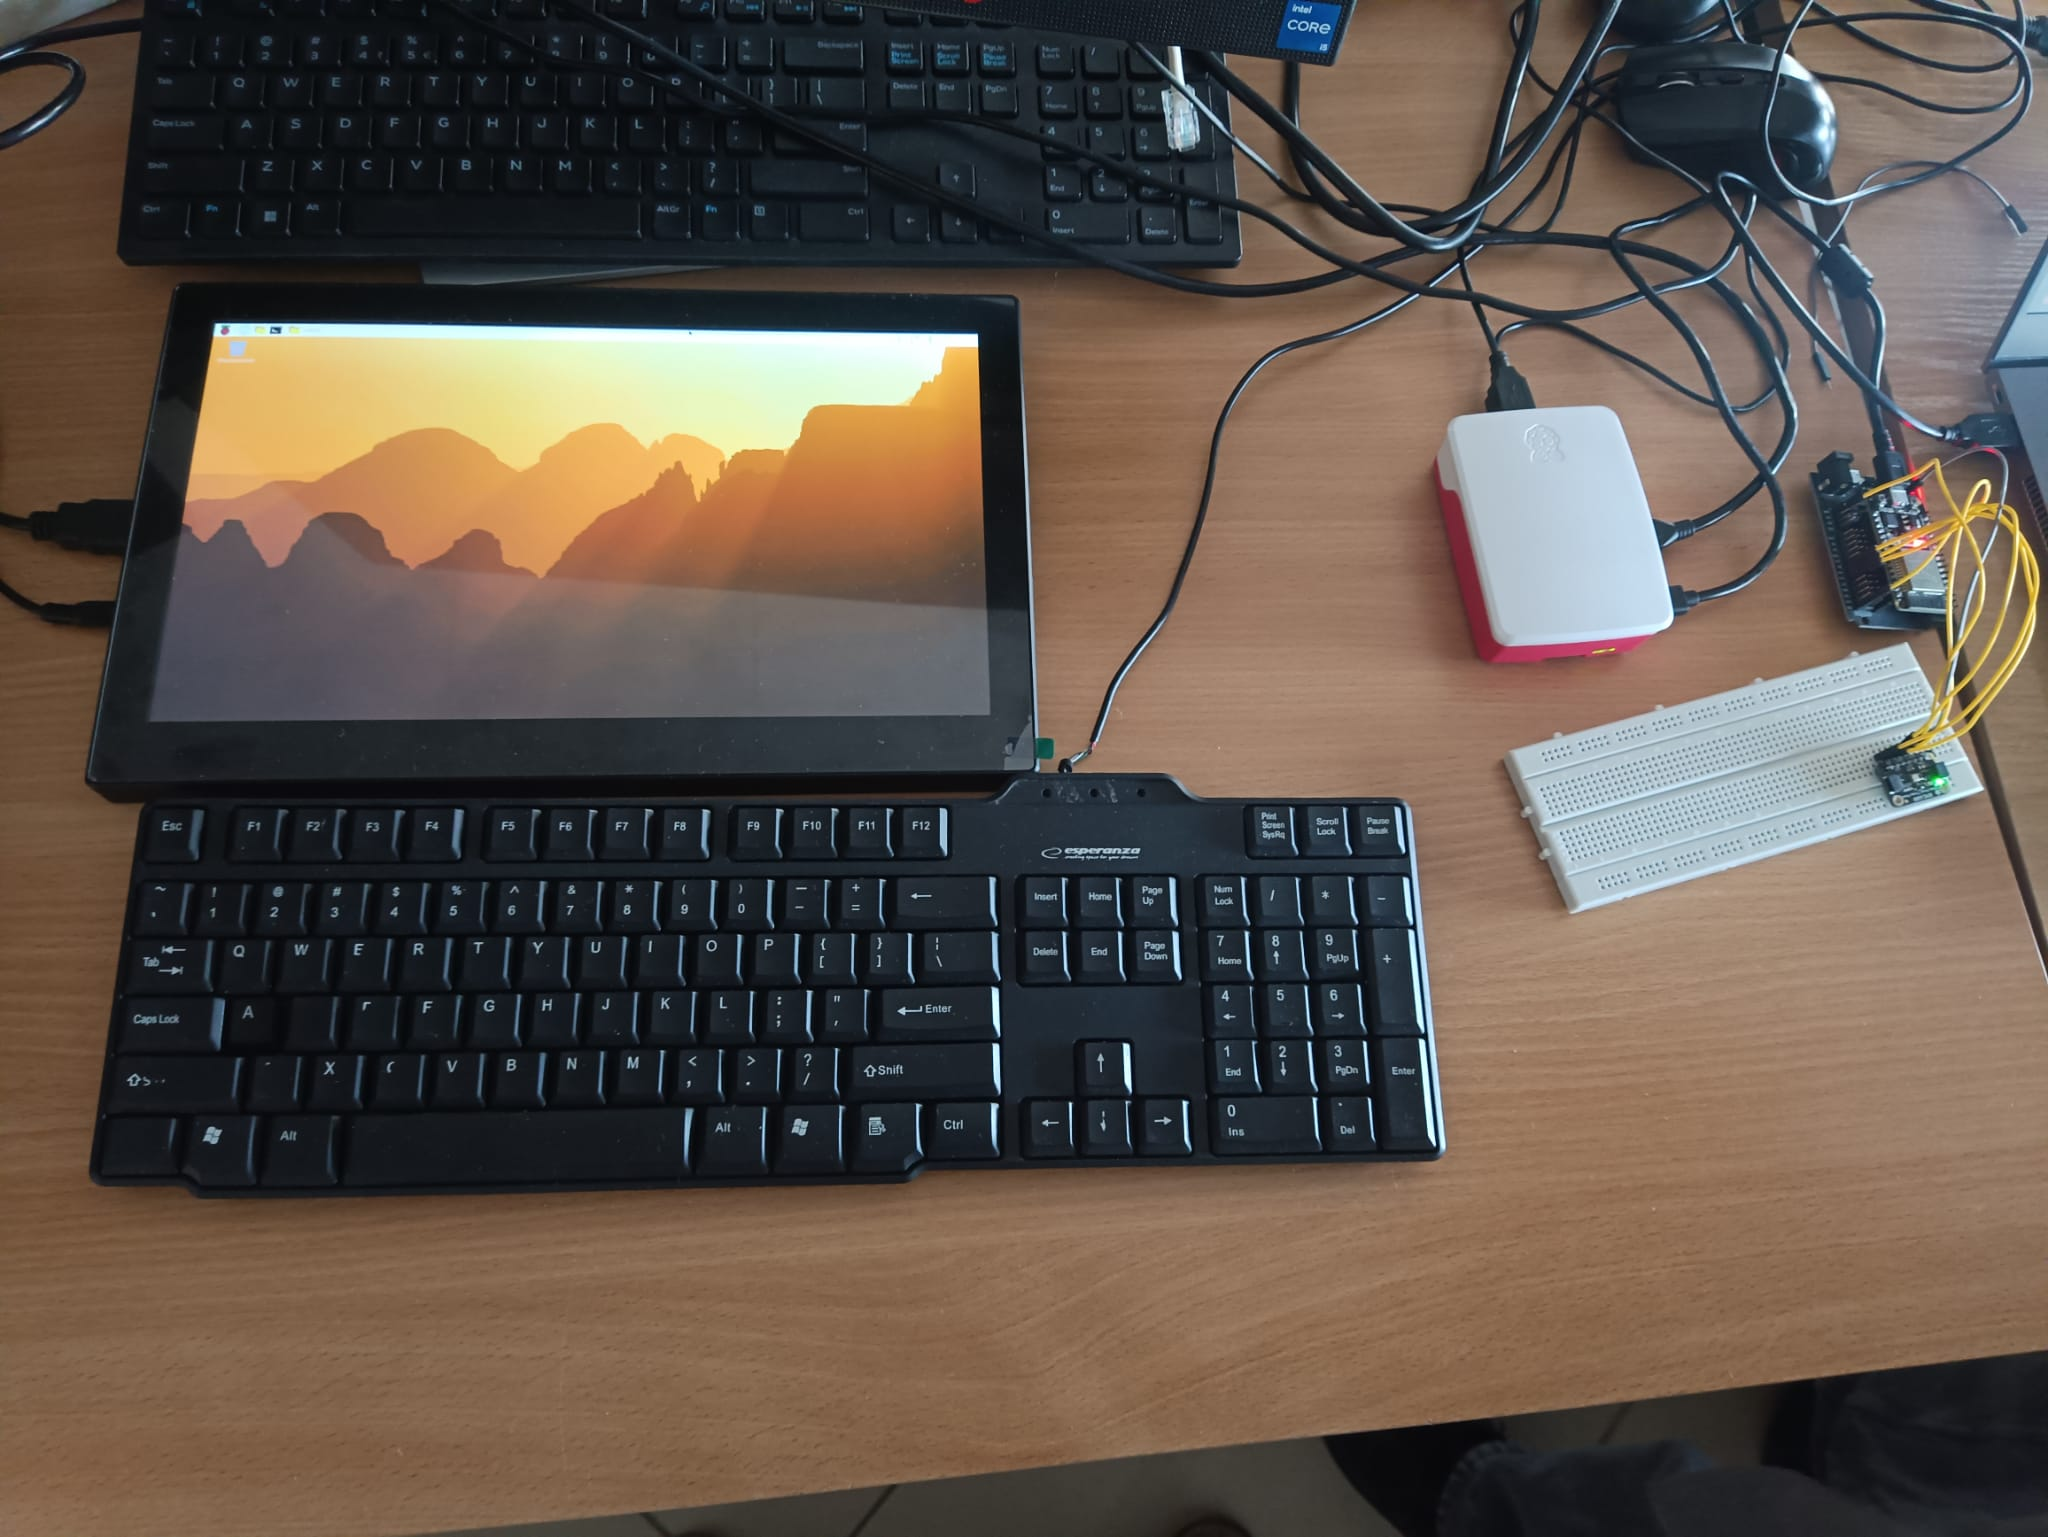
\includegraphics[width=0.95\textwidth]{p3_full_setup.jpg}
    \caption{Complete IoT system setup: Raspberry Pi gateway (centre), ESP32 + BME680 node on breadboard (right), monitor and keyboard (left).}
    \label{fig:p3_full_setup}
\end{figure}
 
\section{Broker Configuration for Remote Connections}
 
To allow remote clients (in this case, the ESP32 connected over Wi-Fi) to connect to the Mosquitto broker on the Raspberry Pi, the configuration file \texttt{/etc/mosquitto/mosquitto.conf} was modified by adding the lines shown in Listing~\ref{lst:mosquitto_conf}. The directive \texttt{listener~1883} opens the standard MQTT port on all interfaces, while \texttt{allow\_anonymous true} disables authentication for this educational setup. Figure~\ref{fig:p3_mosquitto_conf} shows the file as edited with GNU \texttt{nano} on the Raspberry Pi.
 
\begin{lstlisting}[caption={Mosquitto configuration file (\texttt{/etc/mosquitto/mosquitto.conf}).}, label={lst:mosquitto_conf}]
# Place your local configuration in /etc/mosquitto/conf.d/
#
# A full description of the configuration file is at
# /usr/share/doc/mosquitto/examples/mosquitto.conf
 
#pid_file /run/mosquitto/mosquitto.pid
 
persistence true
persistence_location /var/lib/mosquitto/
 
log_dest file /var/log/mosquitto/mosquitto.log
 
include_dir /etc/mosquitto/conf.d
listener 1883
allow_anonymous true
\end{lstlisting}
 
\begin{figure}[H]
    \centering
    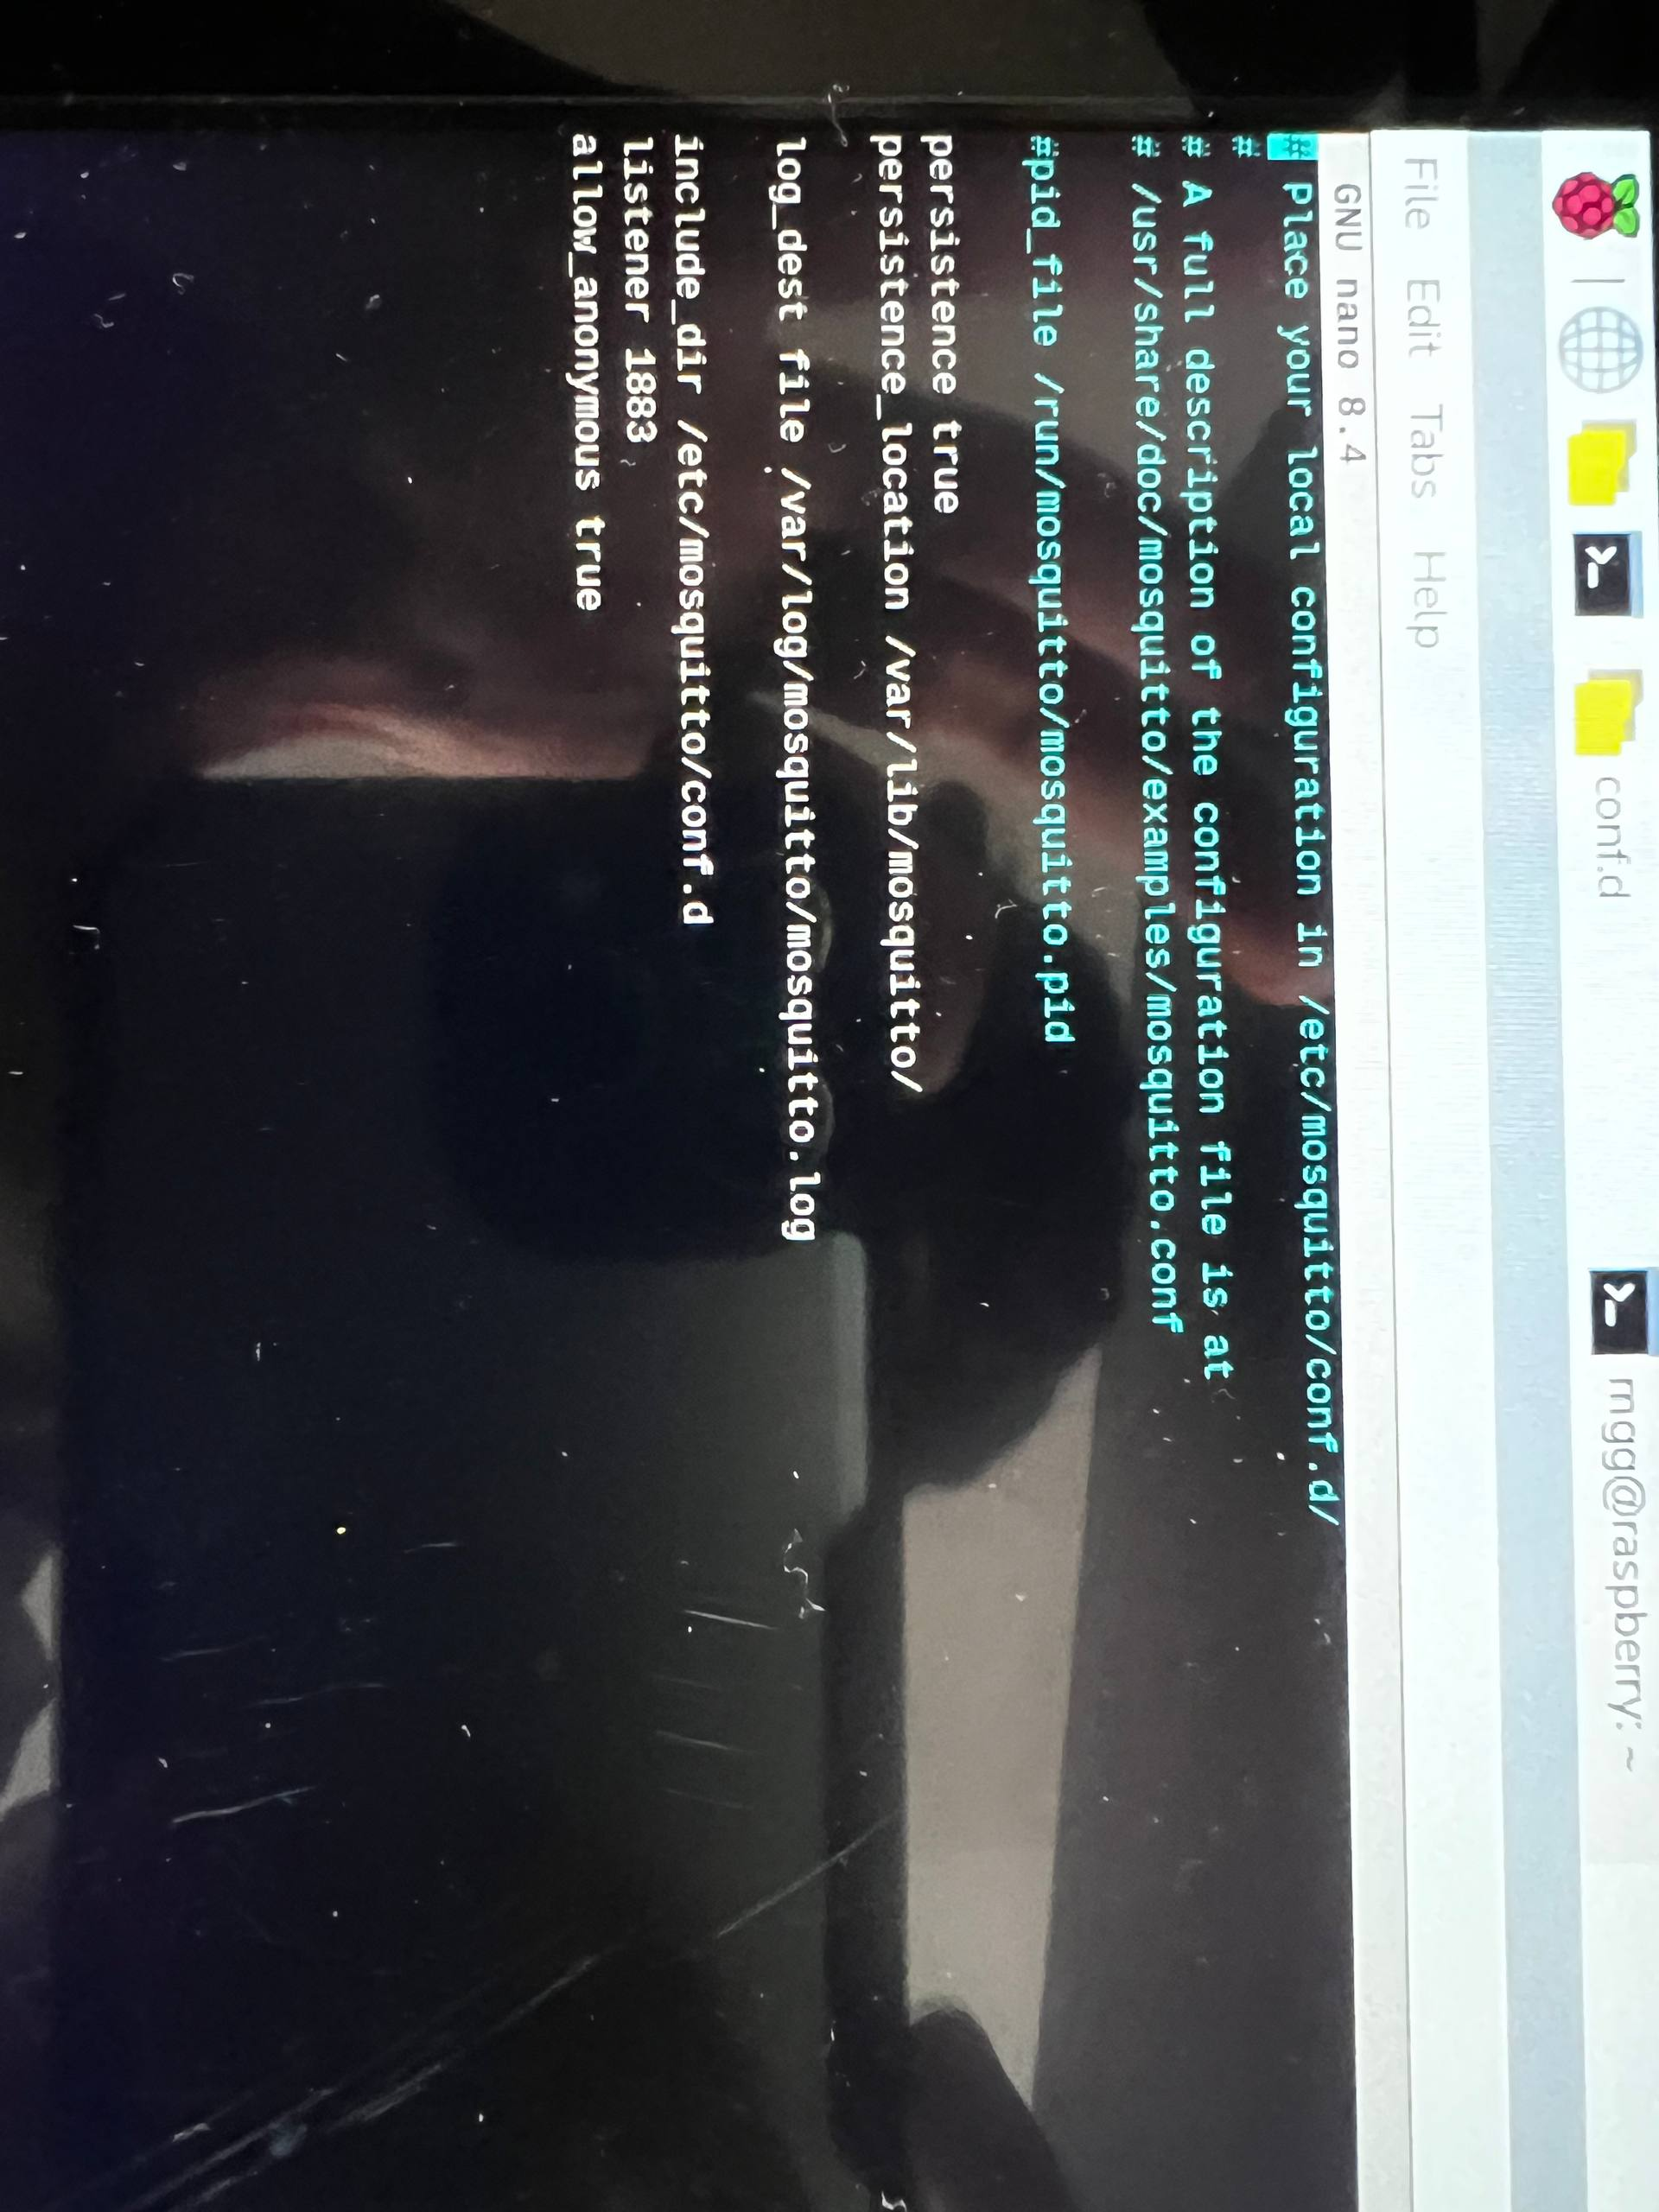
\includegraphics[width=0.80\textwidth, angle=90]{p3_mosquitto_conf.jpg}
    \caption{Mosquitto configuration file edited with GNU \texttt{nano} on the Raspberry Pi.}
    \label{fig:p3_mosquitto_conf}
\end{figure}
 
\section{Code Description}
 
The firmware running on the ESP32 in this part is a re-elaboration of the one developed in Part~1: instead of exposing the sensor data through HTTP, the node connects to the local Wi-Fi network as a client (no longer as an access point), then connects to the Mosquitto broker on the Raspberry Pi and publishes the readings on the topic \texttt{system/1234/data}. The payload is built as a JSON object containing all five quantities (temperature, pressure, humidity, gas resistance, altitude) and sent every two seconds. On the gateway side, the \texttt{mosquitto\_sub} client is used to subscribe to the topic and print every received message on the terminal.
 
\begin{lstlisting}[language=C++, caption={ESP32 firmware: BME680 readings published over MQTT to the Raspberry Pi broker.}]
#include <Wire.h>
#include <SPI.h>
#include <Adafruit_Sensor.h>
#include "Adafruit_BME680.h"
#include <WiFi.h>
#include <PubSubClient.h>
 
// --- WiFi & MQTT config ---
const char* ssid     = "Pietro";
const char* password = "12345678ab";
const char* mqtt_server = "192.168.188.33"; // RPi's IP address
const char* mqtt_topic  = "system/1234/data";
 
// --- BME680 SPI pins ---
#define BME_SCK  13
#define BME_MISO 12
#define BME_MOSI 11
#define BME_CS   5
#define SEALEVELPRESSURE_HPA (1013.25)
 
Adafruit_BME680 bme(BME_CS);
WiFiClient espClient;
PubSubClient client(espClient);
 
// --- Connect to WiFi ---
void setup_wifi() {
  delay(10);
  Serial.print("Connecting to ");
  Serial.println(ssid);
  WiFi.begin(ssid, password);
  while (WiFi.status() != WL_CONNECTED) {
    delay(500);
    Serial.print(".");
  }
  Serial.println("\nWiFi connected. IP: ");
  Serial.println(WiFi.localIP());
}
 
// --- Reconnect to MQTT broker if disconnected ---
void reconnect() {
  while (!client.connected()) {
    Serial.print("Connecting to MQTT broker...");
    if (client.connect("ESP32Client")) {  // unique client ID
      Serial.println("connected!");
    } else {
      Serial.print("failed, rc=");
      Serial.print(client.state());
      Serial.println(" -- retrying in 5s");
      delay(5000);
    }
  }
}
 
void setup() {
  Serial.begin(115200);
  setup_wifi();
  client.setServer(mqtt_server, 1883);
 
  Serial.println("BME680 test");
  if (!bme.begin()) {
    Serial.println("Could not find a valid BME680 sensor, check wiring!");
    while (1);
  }
 
  bme.setTemperatureOversampling(BME680_OS_8X);
  bme.setHumidityOversampling(BME680_OS_2X);
  bme.setPressureOversampling(BME680_OS_4X);
  bme.setIIRFilterSize(BME680_FILTER_SIZE_3);
  bme.setGasHeater(320, 150);
}
 
void loop() {
  if (!client.connected()) reconnect();
  client.loop();
 
  if (!bme.performReading()) {
    Serial.println("Failed to perform reading :(");
    return;
  }
 
  // Build a JSON payload
  char payload[200];
  snprintf(payload, sizeof(payload),
    "{\"temperature\":%.2f,\"pressure\":%.2f,\"humidity\":%.2f,\"gas\":%.2f,\"altitude\":%.2f}",
    bme.temperature,
    bme.pressure / 100.0,
    bme.humidity,
    bme.gas_resistance / 1000.0,
    bme.readAltitude(SEALEVELPRESSURE_HPA)
  );
 
  Serial.print("Publishing: ");
  Serial.println(payload);
  client.publish(mqtt_topic, payload);
 
  delay(2000);
}
\end{lstlisting}
 
On the Raspberry Pi side, the subscription to the topic is performed with the following one-line command:
 
\begin{lstlisting}[language=bash, caption={Raspberry Pi MQTT subscriber command.}]
mosquitto_sub -h localhost -t "system/1234/data"
\end{lstlisting}
 
\section{Results}
 
The ESP32 successfully connected to the local Wi-Fi network and to the Mosquitto broker on the Raspberry Pi at the first attempt. As shown in Figure~\ref{fig:p3_arduino_publish}, the Arduino IDE Serial Monitor confirms a stable MQTT connection (\texttt{Connecting to MQTT broker...connected!}) and a continuous stream of \texttt{Publishing:} messages, each containing a fresh JSON payload with the five environmental quantities sampled every two seconds.
 
\begin{figure}[H]
    \centering
    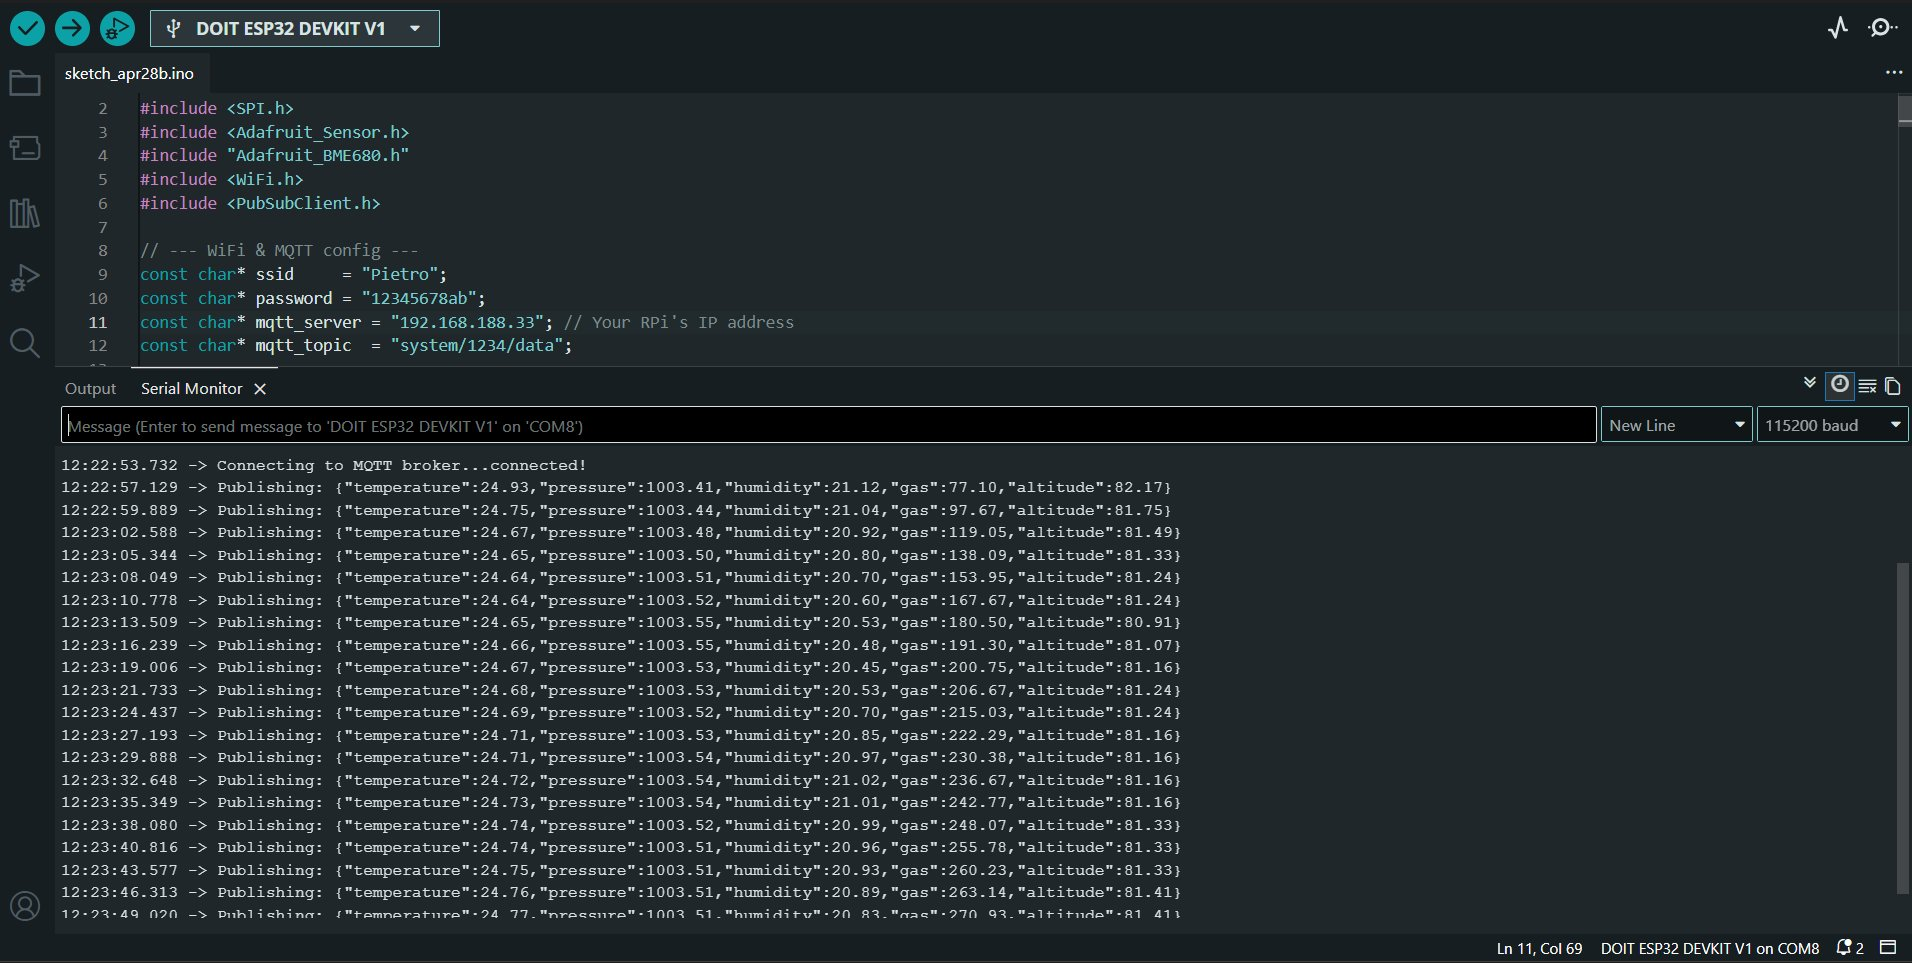
\includegraphics[width=0.95\textwidth]{p3_arduino_publish.png}
    \caption{Arduino IDE Serial Monitor showing the ESP32 publishing JSON payloads to the broker.}
    \label{fig:p3_arduino_publish}
\end{figure}
 
On the Raspberry Pi side, the \texttt{mosquitto\_sub} client (Figure~\ref{fig:p3_sub_cmd}) received the same JSON messages in real time, as shown in Figure~\ref{fig:p3_sub_data}. The two streams are perfectly aligned in content (same temperature, pressure, humidity, gas resistance and altitude values) and only differ by the network propagation time, which is in the order of a few milliseconds on the local network. This proves that the full IoT pipeline, from the BME680 sensor up to the gateway terminal, is correctly working end-to-end.
 
\begin{figure}[H]
    \centering
    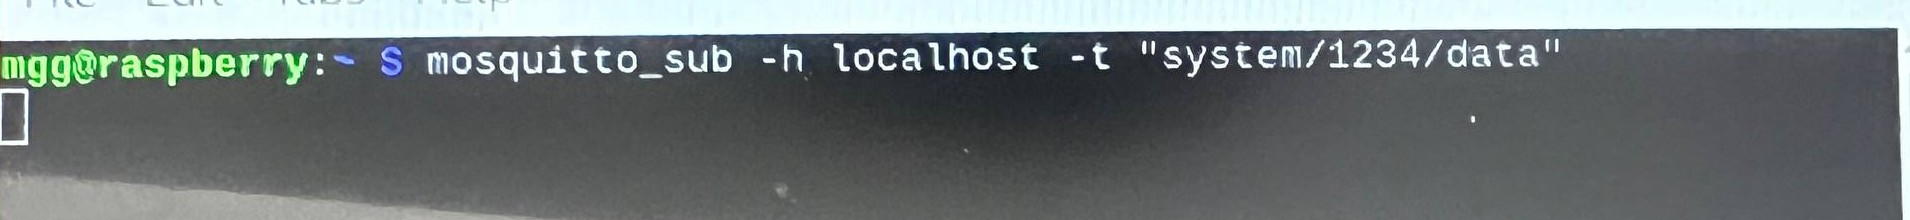
\includegraphics[width=0.95\textwidth]{p3_sub_cmd.jpg}
    \caption{\texttt{mosquitto\_sub} command issued on the Raspberry Pi terminal to listen on the topic \texttt{system/1234/data}.}
    \label{fig:p3_sub_cmd}
\end{figure}
 
\begin{figure}[H]
    \centering
    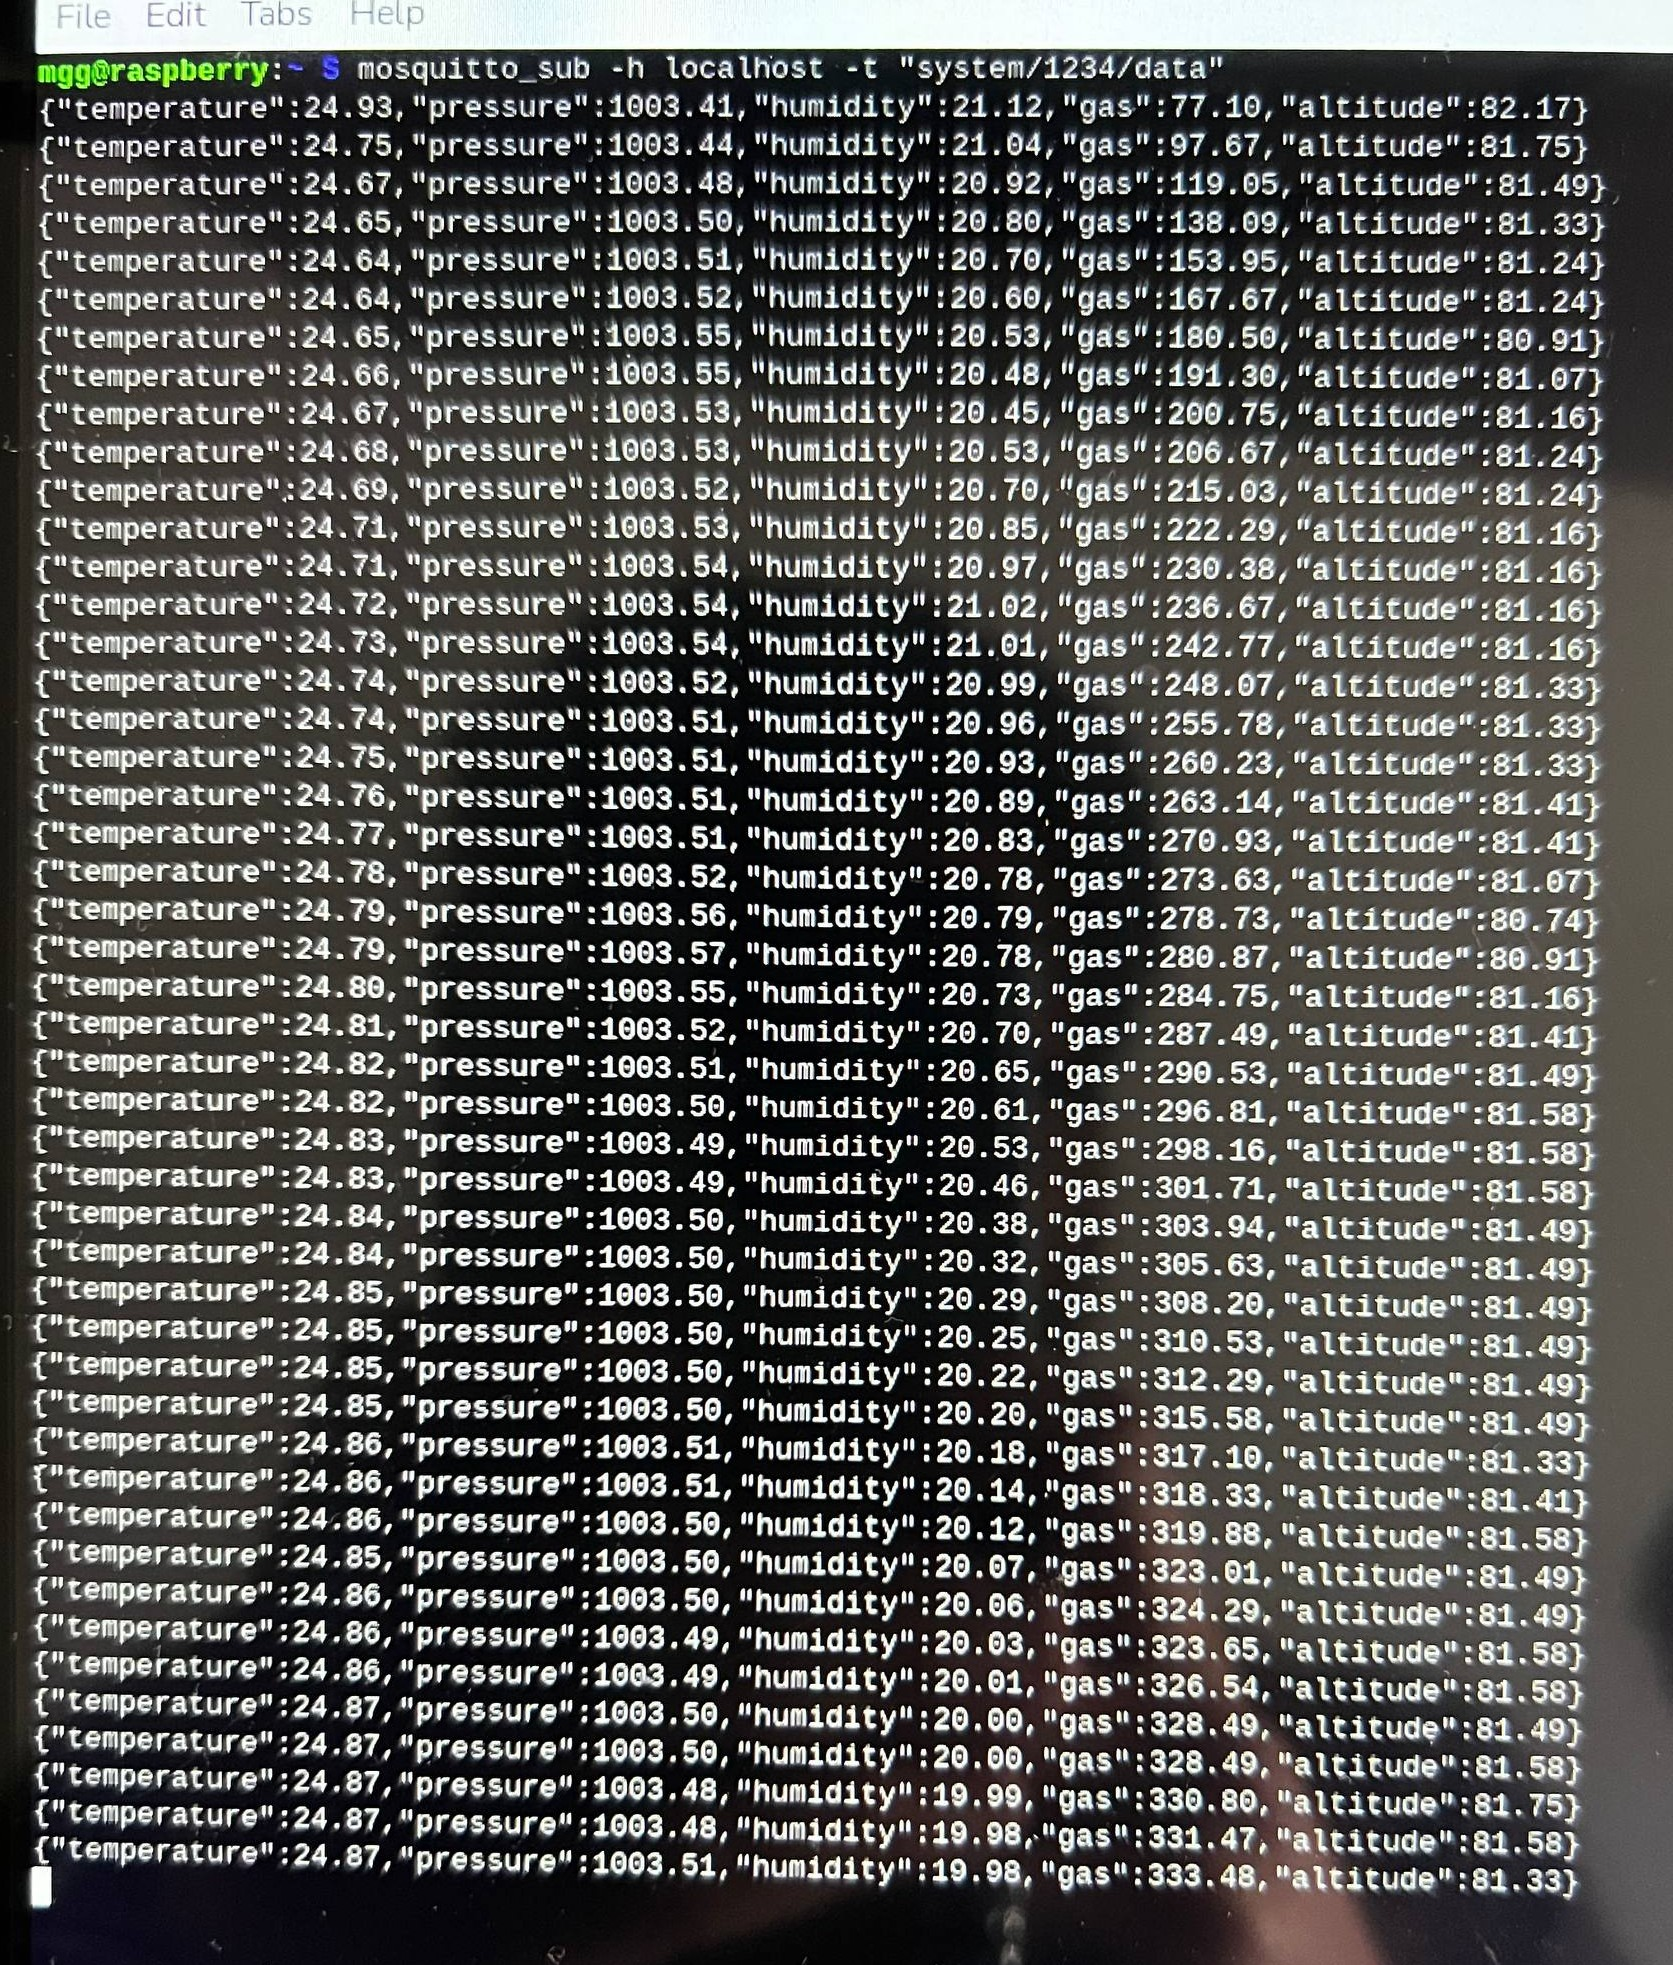
\includegraphics[width=0.95\textwidth]{p3_sub_data.jpg}
    \caption{Sensor data received on the Raspberry Pi by the \texttt{mosquitto\_sub} client subscribed to \texttt{system/1234/data}.}
    \label{fig:p3_sub_data}
\end{figure}
 
A representative excerpt of the received messages is reported below to show the structure of the published payload and the typical magnitude of the readings (temperature near \mbox{24.8\,\textdegree C}, pressure near \mbox{1003.5\,hPa}, humidity around \mbox{20\,\%}, gas resistance progressively increasing as the gas-heating element of the BME680 stabilizes, altitude near \mbox{81\,m}):
 
\begin{lstlisting}[caption={Example of MQTT messages received by \texttt{mosquitto\_sub}.}]
{"temperature":24.93,"pressure":1003.41,"humidity":21.12,"gas":77.10,"altitude":82.17}
{"temperature":24.75,"pressure":1003.44,"humidity":21.04,"gas":97.67,"altitude":81.75}
{"temperature":24.67,"pressure":1003.48,"humidity":20.92,"gas":119.05,"altitude":81.49}
{"temperature":24.65,"pressure":1003.50,"humidity":20.80,"gas":138.09,"altitude":81.33}
{"temperature":24.64,"pressure":1003.51,"humidity":20.70,"gas":153.95,"altitude":81.24}
...
{"temperature":24.87,"pressure":1003.51,"humidity":19.98,"gas":333.48,"altitude":81.33}
\end{lstlisting}
 
The connection remained stable for several minutes of continuous operation, with no message loss observed on the subscriber side and an end-to-end latency low enough to consider the system suitable for real-time environmental monitoring.
 
%==================================================================
\chapter{Conclusions}
%==================================================================
 
The laboratory provided a practical experience of the design and implementation of a complete Internet of Things system, starting from the basic building blocks and progressively integrating them into a single architecture. In Part~1, an ESP32 microcontroller was successfully interfaced with a BME680 environmental sensor and configured to expose the readings through HTTP, demonstrating how a microcontroller can act as a small web server. The development was carried out in three incremental sub-steps -- sensor reading, Wi-Fi access point with HTTP server, and the integrated dashboard -- which made debugging and validation considerably easier. In Part~2, a Raspberry Pi was configured as a gateway running the Mosquitto MQTT broker, and the publish/subscribe mechanism was validated locally with a simple ``Hello world!'' test message. Finally, in Part~3, the two subsystems were integrated: the configuration of \texttt{mosquitto.conf} (opening port 1883 and allowing anonymous connections) made the broker reachable from the ESP32 across the Wi-Fi network, and the node was reprogrammed to publish its sensor data over MQTT to the broker. A client on the gateway received the data in real time and printed them as structured JSON objects.
 
From a learning point of view, the experience showed that the strength of the IoT paradigm lies in the combination of relatively simple components -- a microcontroller, a sensor, a single-board computer, a broker -- arranged into a layered architecture in which each component has a clear and well-defined role. The use of standard protocols (Wi-Fi, HTTP, MQTT) makes the system modular and scalable: additional nodes can be added simply by configuring them to publish to new topics, without changing the gateway or the existing nodes. The wildcard subscription \texttt{system/+/data} used during the laboratory is in fact a direct demonstration of this scalability, as it would allow a single subscriber to receive data from an arbitrary number of sensor nodes identified by their own ID. Possible future extensions of this work include the addition of multiple nodes, the storage of received data in a local database, and the development of a web dashboard for visualization, which would complete the application layer of the IoT architecture introduced at the beginning of this report.
 
\end{document}
 